\documentclass[]{article}
\usepackage{lmodern}
\usepackage{amssymb,amsmath}
\usepackage{ifxetex,ifluatex}
\usepackage{fixltx2e} % provides \textsubscript
\ifnum 0\ifxetex 1\fi\ifluatex 1\fi=0 % if pdftex
  \usepackage[T1]{fontenc}
  \usepackage[utf8]{inputenc}
\else % if luatex or xelatex
  \ifxetex
    \usepackage{mathspec}
  \else
    \usepackage{fontspec}
  \fi
  \defaultfontfeatures{Ligatures=TeX,Scale=MatchLowercase}
\fi
% use upquote if available, for straight quotes in verbatim environments
\IfFileExists{upquote.sty}{\usepackage{upquote}}{}
% use microtype if available
\IfFileExists{microtype.sty}{%
\usepackage{microtype}
\UseMicrotypeSet[protrusion]{basicmath} % disable protrusion for tt fonts
}{}
\usepackage[margin=1in]{geometry}
\usepackage{hyperref}
\hypersetup{unicode=true,
            pdftitle={Oregon Extended Analyses: 2019},
            pdfauthor={Brock Rowley; Sevrina Tindal; Philip Irvin; Daniel Anderson; Gerald Tindal},
            pdfborder={0 0 0},
            breaklinks=true}
\urlstyle{same}  % don't use monospace font for urls
\usepackage{color}
\usepackage{fancyvrb}
\newcommand{\VerbBar}{|}
\newcommand{\VERB}{\Verb[commandchars=\\\{\}]}
\DefineVerbatimEnvironment{Highlighting}{Verbatim}{commandchars=\\\{\}}
% Add ',fontsize=\small' for more characters per line
\usepackage{framed}
\definecolor{shadecolor}{RGB}{248,248,248}
\newenvironment{Shaded}{\begin{snugshade}}{\end{snugshade}}
\newcommand{\AlertTok}[1]{\textcolor[rgb]{0.94,0.16,0.16}{#1}}
\newcommand{\AnnotationTok}[1]{\textcolor[rgb]{0.56,0.35,0.01}{\textbf{\textit{#1}}}}
\newcommand{\AttributeTok}[1]{\textcolor[rgb]{0.77,0.63,0.00}{#1}}
\newcommand{\BaseNTok}[1]{\textcolor[rgb]{0.00,0.00,0.81}{#1}}
\newcommand{\BuiltInTok}[1]{#1}
\newcommand{\CharTok}[1]{\textcolor[rgb]{0.31,0.60,0.02}{#1}}
\newcommand{\CommentTok}[1]{\textcolor[rgb]{0.56,0.35,0.01}{\textit{#1}}}
\newcommand{\CommentVarTok}[1]{\textcolor[rgb]{0.56,0.35,0.01}{\textbf{\textit{#1}}}}
\newcommand{\ConstantTok}[1]{\textcolor[rgb]{0.00,0.00,0.00}{#1}}
\newcommand{\ControlFlowTok}[1]{\textcolor[rgb]{0.13,0.29,0.53}{\textbf{#1}}}
\newcommand{\DataTypeTok}[1]{\textcolor[rgb]{0.13,0.29,0.53}{#1}}
\newcommand{\DecValTok}[1]{\textcolor[rgb]{0.00,0.00,0.81}{#1}}
\newcommand{\DocumentationTok}[1]{\textcolor[rgb]{0.56,0.35,0.01}{\textbf{\textit{#1}}}}
\newcommand{\ErrorTok}[1]{\textcolor[rgb]{0.64,0.00,0.00}{\textbf{#1}}}
\newcommand{\ExtensionTok}[1]{#1}
\newcommand{\FloatTok}[1]{\textcolor[rgb]{0.00,0.00,0.81}{#1}}
\newcommand{\FunctionTok}[1]{\textcolor[rgb]{0.00,0.00,0.00}{#1}}
\newcommand{\ImportTok}[1]{#1}
\newcommand{\InformationTok}[1]{\textcolor[rgb]{0.56,0.35,0.01}{\textbf{\textit{#1}}}}
\newcommand{\KeywordTok}[1]{\textcolor[rgb]{0.13,0.29,0.53}{\textbf{#1}}}
\newcommand{\NormalTok}[1]{#1}
\newcommand{\OperatorTok}[1]{\textcolor[rgb]{0.81,0.36,0.00}{\textbf{#1}}}
\newcommand{\OtherTok}[1]{\textcolor[rgb]{0.56,0.35,0.01}{#1}}
\newcommand{\PreprocessorTok}[1]{\textcolor[rgb]{0.56,0.35,0.01}{\textit{#1}}}
\newcommand{\RegionMarkerTok}[1]{#1}
\newcommand{\SpecialCharTok}[1]{\textcolor[rgb]{0.00,0.00,0.00}{#1}}
\newcommand{\SpecialStringTok}[1]{\textcolor[rgb]{0.31,0.60,0.02}{#1}}
\newcommand{\StringTok}[1]{\textcolor[rgb]{0.31,0.60,0.02}{#1}}
\newcommand{\VariableTok}[1]{\textcolor[rgb]{0.00,0.00,0.00}{#1}}
\newcommand{\VerbatimStringTok}[1]{\textcolor[rgb]{0.31,0.60,0.02}{#1}}
\newcommand{\WarningTok}[1]{\textcolor[rgb]{0.56,0.35,0.01}{\textbf{\textit{#1}}}}
\usepackage{graphicx,grffile}
\makeatletter
\def\maxwidth{\ifdim\Gin@nat@width>\linewidth\linewidth\else\Gin@nat@width\fi}
\def\maxheight{\ifdim\Gin@nat@height>\textheight\textheight\else\Gin@nat@height\fi}
\makeatother
% Scale images if necessary, so that they will not overflow the page
% margins by default, and it is still possible to overwrite the defaults
% using explicit options in \includegraphics[width, height, ...]{}
\setkeys{Gin}{width=\maxwidth,height=\maxheight,keepaspectratio}
\IfFileExists{parskip.sty}{%
\usepackage{parskip}
}{% else
\setlength{\parindent}{0pt}
\setlength{\parskip}{6pt plus 2pt minus 1pt}
}
\setlength{\emergencystretch}{3em}  % prevent overfull lines
\providecommand{\tightlist}{%
  \setlength{\itemsep}{0pt}\setlength{\parskip}{0pt}}
\setcounter{secnumdepth}{0}
% Redefines (sub)paragraphs to behave more like sections
\ifx\paragraph\undefined\else
\let\oldparagraph\paragraph
\renewcommand{\paragraph}[1]{\oldparagraph{#1}\mbox{}}
\fi
\ifx\subparagraph\undefined\else
\let\oldsubparagraph\subparagraph
\renewcommand{\subparagraph}[1]{\oldsubparagraph{#1}\mbox{}}
\fi

%%% Use protect on footnotes to avoid problems with footnotes in titles
\let\rmarkdownfootnote\footnote%
\def\footnote{\protect\rmarkdownfootnote}

%%% Change title format to be more compact
\usepackage{titling}

% Create subtitle command for use in maketitle
\providecommand{\subtitle}[1]{
  \posttitle{
    \begin{center}\large#1\end{center}
    }
}

\setlength{\droptitle}{-2em}

  \title{Oregon Extended Analyses: 2019}
    \pretitle{\vspace{\droptitle}\centering\huge}
  \posttitle{\par}
    \author{Brock Rowley \\ Sevrina Tindal \\ Philip Irvin \\ Daniel Anderson \\ Gerald Tindal}
    \preauthor{\centering\large\emph}
  \postauthor{\par}
      \predate{\centering\large\emph}
  \postdate{\par}
    \date{6/29/2019}

\pagenumbering{gobble}
\usepackage{placeins}
\usepackage{float}
\usepackage{caption}
\captionsetup[figure]{labelformat = empty}
\usepackage{xcolor}
\definecolor{link}{rgb}{0, 0, 238}
\usepackage{booktabs}

\begin{document}
\maketitle

{
\setcounter{tocdepth}{5}
\tableofcontents
}
\hypertarget{critical-element-4---technical-quality-other}{%
\subsection{Critical Element 4 - Technical Quality:
Other}\label{critical-element-4---technical-quality-other}}

\hypertarget{reliability}{%
\subsubsection{4.1 Reliability}\label{reliability}}

Test reliability can be viewed through several lenses, all of which
document how consistently an assessment performs across occasions,
contexts, and raters. Typical strategies for addressing reliability
include documentation of internal consistency, split-half reliability,
and test-retest reliability. If multiple forms are implemented, test
form reliability documentation is also requisite. The implementation
plan for the ORExt includes initial documentation of internal
consistency (Cronbach's alpha). The 2015-16 technical report included
internal consistency estimates, split-half reliability analyses, as well
as a small test-retest assessment of reliability comparisons by means of
our pilot tablet administration study. There is only one test form for
the ORExt, so test form comparisons are not possible. \newpage

\hypertarget{inter-rater-reliability}{%
\paragraph{Inter-Rater-Reliability}\label{inter-rater-reliability}}

\hypertarget{background}{%
\subparagraph{Background}\label{background}}

ODE's technical documentation plan (see page 136 in the 2016-17
Technical Report), included an Inter-Rater Reliability (IRR) study for
the 2017-18 school year. Pursuant to Hallgren, K. A. (2012) the
assessment of IRR may be necessary to demonstrate consistency among
observational ratings provided by multiple assessors. The results of the
study will be used to address the requirements within the USED's Peer
Review process (Critical Element 4.1). A sample of Oregon's Qualified
Assessors (QAs) who administer the paper/pencil version of the Oregon
Extended Assessment (ORExt) were observed to determine reliability of
administration and scoring. We did not include the tablet administration
or the Oregon Observational Rating.

\hypertarget{methods}{%
\subparagraph{Methods}\label{methods}}

QTs in districts across the state observe a sample of their respective
QAs using the observation protocol (see \emph{Appendix} 4.1
InterRater\_Observation\_Form) and enter their data online. The QA reads
the item stem and the student selects from three possible answer choices
(A, B, or C) then, the QA records the answer choice. QTs (observer)
records the students answer choice, then records the answer choice
recorded by the QA for agreement. Only the English Language Arts Writing
porting of the ORExt requires additional analysis by the assessor to
determine if the written response (answer) meets (1) or doesn't meet (0)
provided critera. Districts from across the state of Oregon participated
in the study, matching the state's student population demographics,
including large, medium, and small districts, across all regions. The
observation protocol was completed for the identified QA, but the
student(s) and content area(s) observed were selected by the QT or QA.
BRT researchers contacted district-level QTs at the beginning of the
test window, which runs from February 15 - April 26, 2018, to arrange
observations that could hopefully be completed within one school day. In
addition to addressing inter-rater reliability, the study also evaluated
test administration procedures. The methods, results, and interpretation
are provided here, in addition to recommended next steps. The
observation was composed of three sections:

\begin{itemize}
\item
  First, QT's reviewed ORExt paper/pencil test preparation and
  administration using the rubric (Appendix 4.1
  InterRater\_Observation\_Form). Test preparation/administration
  domains were rated on a four-point scale from Inappropriate (I) to
  Exemplary (E):

  \begin{itemize}
  \item
    Inappropriate (I) denotes a level of concern that could clearly
    affect the accuracy of the test results gathered from the test
    administration. Ratings at this level require substantive retraining
    of the QA involved.
  \item
    Somewhat Appropriate (SA) rating denotes a level that includes some
    minor aspects that could be improved, but the accuracy of the test
    results are likely not compromised.
  \item
    Appropriate (A) denotes a level that is consistent with all test
    administration requirements.
  \item
    Exemplary (E) level performance suggests that the QA incorporated
    approaches to test administration that could become models for best
    practice.
  \end{itemize}
\item
  Second, QT's scored the student alongside the QA using the scoring
  sheet. QT's compared results after this observation to ensure that the
  QA entered accurate data.
\item
  Finally, QT's observed the QA completing the data entry process to
  ensure that no errors are made during data entry and document the
  number of errors (Appendix 4.1 InterRater\_Observation\_Form).
\end{itemize}

Domain Definitions

\begin{enumerate}
\def\labelenumi{\arabic{enumi}.}
\item
  Test Security -- The QA utilized a system to ensure that all test
  materials were stored in a secure location,. The QA also had a
  district Assurance of Test Security form on file.
\item
  Printed Materials -- the QA had all materials required to administer
  the ORExt ready for test administration.
\item
  Distraction-Free Environment -- the QA arranged to provide the ORExt
  in a one-on-one test administration in a location that ensured that
  the student focused attention on the assessment.
\item
  Accessibility Supports -- the QA provided all necessary accessibility
  supports for the student and ensured that all support systems were
  functional prior to testing.
\item
  Level of Support -- The QA provided an appropriate level of support
  throughout testing that did not compromise the validity of the score.
\item
  Praise -- The QA utilized praise appropriately to support student
  involvement without leading the student to the correct answer.
\item
  Motivation -- The QA appropriately maintained the student's motivation
  during the assessment using relevant strategies, such as token
  systems.
\item
  Score Interpretation -- The QA demonstrated an appropriate
  understanding of how to use the cut scores and achievement level
  descriptors to interpret scores (i.e., ask the QA to describe how they
  interpret scores for parents).
\item
  Minimum Participation Rule - The QA demonstrated an appropriate
  understanding of the minimum participation rule (i.e., ask the QA to
  define the rule if it is not used).
\end{enumerate}

Qualified Assessor Testing Preparation and Administration Rubric (Record
an ``X'' in the cell that corresponds to your rating)

\FloatBarrier

\includegraphics{Figures/irr/irr_domain.png}

\FloatBarrier

\hypertarget{inter-rater-agreement-results}{%
\subparagraph{Inter-rater Agreement
Results}\label{inter-rater-agreement-results}}

Thirty-three Qualified Trainers from around Oregon participated in the
Inter-Rater-Reliability study by doing at least one observation on the
Oregon Extended Assessment via paper/pencil administration. Of the
thirty-three observations, 48.5\% were English Language Arts, 33.3\%
were Mathematics, and 18.2\% were Science. Observations were done at
individual student's typical testing location. The study found a 99.3
Inter-Rater Reliability percentage agreement between the test observers
and test administrators on student item (answer) selection.

The following two tables (Table 21 and Table 22) display the percentage
of reponses in the nine different domains and percentage of agreement
between assessors and observers. \FloatBarrier

\begin{Shaded}
\begin{Highlighting}[]
\KeywordTok{library}\NormalTok{(tidyverse)}
\KeywordTok{library}\NormalTok{(fs)}
\KeywordTok{library}\NormalTok{(rio)}
\KeywordTok{library}\NormalTok{(RColorBrewer)}

\NormalTok{d <-}\StringTok{ }\KeywordTok{import}\NormalTok{(}\StringTok{"data/irr/RaterReliability.csv"}\NormalTok{, }\DataTypeTok{setclass =} \StringTok{"tbl_df"}\NormalTok{) }\OperatorTok\StringTok{ }
\StringTok{  }\NormalTok{janitor}\OperatorTok{::}\KeywordTok{clean_names}\NormalTok{()}

\KeywordTok{theme_set}\NormalTok{(}\KeywordTok{theme_minimal}\NormalTok{())}
  \CommentTok{# Percentage for responses    }
\NormalTok{d }\OperatorTok\StringTok{ }
\StringTok{  }\KeywordTok{gather}\NormalTok{(var, response, test_security}\OperatorTok{:}\NormalTok{minimum_participation) }\OperatorTok\StringTok{ }
\StringTok{  }\KeywordTok{group_by}\NormalTok{(var) }\OperatorTok
\StringTok{  }\KeywordTok{count}\NormalTok{(response)}\OperatorTok
\StringTok{  }\KeywordTok{mutate}\NormalTok{(}\DataTypeTok{tot =} \KeywordTok{sum}\NormalTok{(n),}
         \DataTypeTok{percent =}\NormalTok{ (n}\OperatorTok{/}\NormalTok{tot)}\OperatorTok{*}\DecValTok{100}\NormalTok{) }\OperatorTok\StringTok{ }
\StringTok{  }\KeywordTok{select}\NormalTok{(}\OperatorTok{-}\NormalTok{n, }\OperatorTok{-}\NormalTok{tot) }\OperatorTok\StringTok{ }
\StringTok{  }\KeywordTok{spread}\NormalTok{(response, percent, }\DataTypeTok{fill =} \DecValTok{0}\NormalTok{) }\OperatorTok\StringTok{ }
\StringTok{  }\KeywordTok{select}\NormalTok{(Exemplary, Appropriate, }\StringTok{`}\DataTypeTok{Somewhat Appropriate}\StringTok{`}\NormalTok{, Inappropriate)}\OperatorTok
\StringTok{  }\KeywordTok{kable}\NormalTok{(}\StringTok{"latex"}\NormalTok{, }
        \DataTypeTok{booktabs =} \OtherTok{TRUE}\NormalTok{,}
        \DataTypeTok{caption =} \StringTok{"Percentage for responses"}\NormalTok{,}
        \DataTypeTok{digits =} \DecValTok{2}\NormalTok{) }\OperatorTok\StringTok{ }
\StringTok{        }\KeywordTok{kable_styling}\NormalTok{(}\DataTypeTok{full_width =} \OtherTok{TRUE}\NormalTok{,}
                      \DataTypeTok{latex_options =} \StringTok{"hold_position"}\NormalTok{)}
\CommentTok{# Proportion of respondents who provide a rating of "Mark As Disagree"}
\NormalTok{d }\OperatorTok\StringTok{ }
\StringTok{  }\KeywordTok{select}\NormalTok{(}\KeywordTok{starts_with}\NormalTok{(}\StringTok{"item"}\NormalTok{)) }\OperatorTok\StringTok{ }
\StringTok{  }\KeywordTok{gather}\NormalTok{(item, response) }\OperatorTok\StringTok{ }
\StringTok{  }\KeywordTok{count}\NormalTok{(response) }\OperatorTok\StringTok{ }
\StringTok{  }\KeywordTok{mutate}\NormalTok{(}\DataTypeTok{tot =} \KeywordTok{sum}\NormalTok{(n),}
         \DataTypeTok{percent =}\NormalTok{ (n}\OperatorTok{/}\NormalTok{tot)}\OperatorTok{*}\DecValTok{100}\NormalTok{)}\OperatorTok
\KeywordTok{kable}\NormalTok{(}\StringTok{"latex"}\NormalTok{, }
        \DataTypeTok{booktabs =} \OtherTok{TRUE}\NormalTok{,}
        \DataTypeTok{caption =} \StringTok{"Mark As Disagree"}\NormalTok{,}
        \DataTypeTok{digits =} \DecValTok{2}\NormalTok{) }\OperatorTok\StringTok{ }
\StringTok{        }\KeywordTok{kable_styling}\NormalTok{(}\DataTypeTok{full_width =} \OtherTok{TRUE}\NormalTok{,}
                      \DataTypeTok{latex_options =} \StringTok{"hold_position"}\NormalTok{)}
\end{Highlighting}
\end{Shaded}

\clearpage
\FloatBarrier

The following table provides a visual display of the responses from the
nine differnt domains observed.

\begin{Shaded}
\begin{Highlighting}[]
\KeywordTok{library}\NormalTok{(tidyverse)}
\KeywordTok{library}\NormalTok{(fs)}
\KeywordTok{library}\NormalTok{(rio)}
\KeywordTok{library}\NormalTok{(RColorBrewer)}


\NormalTok{d <-}\StringTok{ }\KeywordTok{import}\NormalTok{(}\StringTok{"data/irr/RaterReliability.csv"}\NormalTok{, }\DataTypeTok{setclass =} \StringTok{"tbl_df"}\NormalTok{) }\OperatorTok\StringTok{ }
\StringTok{  }\NormalTok{janitor}\OperatorTok{::}\KeywordTok{clean_names}\NormalTok{()}

\KeywordTok{theme_set}\NormalTok{(}\KeywordTok{theme_minimal}\NormalTok{())}
\CommentTok{# Counts for responses}
\NormalTok{d }\OperatorTok\StringTok{ }
\StringTok{  }\KeywordTok{gather}\NormalTok{(var, response, test_security}\OperatorTok{:}\NormalTok{minimum_participation) }\OperatorTok\StringTok{ }
\StringTok{  }\KeywordTok{group_by}\NormalTok{(var) }\OperatorTok
\StringTok{  }\KeywordTok{count}\NormalTok{(response) }\OperatorTok
\StringTok{  }\KeywordTok{mutate}\NormalTok{(}\DataTypeTok{response =} \KeywordTok{factor}\NormalTok{(response, }
                           \DataTypeTok{levels =} \KeywordTok{c}\NormalTok{(}\StringTok{"Exemplary"}\NormalTok{, }
                                      \StringTok{"Appropriate"}\NormalTok{, }
                                      \StringTok{"Somewhat Appropriate"}\NormalTok{,}
                                      \StringTok{"Inappropriate"}\NormalTok{))) }\OperatorTok\StringTok{ }
\StringTok{  }\KeywordTok{ggplot}\NormalTok{(}\KeywordTok{aes}\NormalTok{(response, n)) }\OperatorTok{+}
\StringTok{  }\KeywordTok{geom_col}\NormalTok{(}\KeywordTok{aes}\NormalTok{(}\DataTypeTok{fill =}\NormalTok{ response)) }\OperatorTok{+}
\StringTok{  }\KeywordTok{scale_fill_brewer}\NormalTok{(}\DataTypeTok{palette =} \StringTok{"Set1"}\NormalTok{) }\OperatorTok{+}
\StringTok{  }\KeywordTok{facet_wrap}\NormalTok{(}\OperatorTok{~}\NormalTok{var, }\DataTypeTok{labeller =}\NormalTok{ label_parsed) }\OperatorTok{+}
\StringTok{  }\KeywordTok{guides}\NormalTok{(}\DataTypeTok{fill =} \StringTok{"none"}\NormalTok{) }\OperatorTok{+}
\StringTok{  }\KeywordTok{labs}\NormalTok{(}\DataTypeTok{x =} \StringTok{""}\NormalTok{) }\OperatorTok{+}
\StringTok{  }\KeywordTok{labs}\NormalTok{(}\DataTypeTok{y =} \StringTok{""}\NormalTok{) }\OperatorTok{+}
\StringTok{  }\KeywordTok{theme}\NormalTok{(}\DataTypeTok{axis.text.x =} \KeywordTok{element_text}\NormalTok{(}\DataTypeTok{angle =} \DecValTok{45}\NormalTok{, }\DataTypeTok{vjust =} \FloatTok{0.5}\NormalTok{, }\DataTypeTok{hjust=}\DecValTok{1}\NormalTok{))}
\end{Highlighting}
\end{Shaded}

Results:

ORExt's Selected response format provides for a high percentage of
inter-rater reliability. One resonse out of the 1200 observed where
observes disagreed with rateres was in the ELA Writing scoring. `Score
Interpretation' appears to be a domain in need of additional training.
Qualified Trainers indicated that 16\% of observed Qualified Assessors
were Somewhat Appropriate and 8\% were Inappropriate in their
understanding of how to use cut scores and achievement level descriptors
to interpret scores.

Next Steps and Recommendations:

Additional training should be provided on the QT/QA training site to
ensure QT's and QA's and using the scoring rubric provided for ELA
Writing items and appropriately scoring ELA Writing. Samples from the
different types of ELA Writing should itme promps should be use during
the QT/QA proficiency assessment to ensure consistency between all who
administer the ORExt. Score Interpretation training should be
incoporated into QT training slides and disiminated in QA training. Any
score interpretation guide section of QT training may need to be
revisited to ensure clarity around achievement level descriptors.

\hypertarget{a-test-reliability}{%
\paragraph{4.1A Test Reliability}\label{a-test-reliability}}

Marginal reliability results (true score variance/true score variance +
error variance) demonstrate that the tests are quite reliable at the
total test level. Full reliability statistics for each of the
operational tests administered this year are provided below. These
results demonstrate that the total test reliabilities were quite high,
ranging from .67 to .91. Each table below provides the content area,
grade, and the marginal reliabilities. All test forms were composed of
36 operational and 12 embedded field-test items.

\begin{Shaded}
\begin{Highlighting}[]
\NormalTok{marg_rel <-}\StringTok{ }\ControlFlowTok{function}\NormalTok{(theta, se) \{}
\NormalTok{  s <-}\StringTok{ }\KeywordTok{var}\NormalTok{(theta)}
\NormalTok{  e <-}\StringTok{ }\KeywordTok{mean}\NormalTok{((se)}\OperatorTok{^}\DecValTok{2}\NormalTok{)}
\NormalTok{  s}\OperatorTok{/}\NormalTok{(s}\OperatorTok{+}\NormalTok{e)}
\NormalTok{\}}
\NormalTok{tbls <-}\StringTok{ }\NormalTok{ode }\OperatorTok\StringTok{ }
\StringTok{  }\KeywordTok{group_by}\NormalTok{(content_area, grade) }\OperatorTok\StringTok{ }
\StringTok{  }\KeywordTok{summarize}\NormalTok{(}\DataTypeTok{marg_rel =} \KeywordTok{marg_rel}\NormalTok{(theta, se)) }\OperatorTok\StringTok{ }
\StringTok{  }\KeywordTok{rename}\NormalTok{(}\DataTypeTok{Grade =}\NormalTok{ grade, }
         \StringTok{`}\DataTypeTok{Marginal Reliability Estimate}\StringTok{`}\NormalTok{ =}\StringTok{ }\NormalTok{marg_rel) }\OperatorTok\StringTok{ }
\StringTok{  }\KeywordTok{split}\NormalTok{(.}\OperatorTok{$}\NormalTok{content_area) }\OperatorTok\StringTok{ }
\StringTok{  }\KeywordTok{map}\NormalTok{(}\OperatorTok{~}\KeywordTok{ungroup}\NormalTok{(.) }\OperatorTok\StringTok{ }\KeywordTok{select}\NormalTok{(}\OperatorTok{-}\NormalTok{content_area))}

\KeywordTok{walk2}\NormalTok{(tbls,}
      \KeywordTok{paste0}\NormalTok{(}\KeywordTok{c}\NormalTok{(}\StringTok{"ELA"}\NormalTok{, }\StringTok{"Math"}\NormalTok{, }\StringTok{"Reading"}\NormalTok{, }\StringTok{"Science"}\NormalTok{, }\StringTok{"Writing"}\NormalTok{),}
             \StringTok{" Marginal Reliabilities"}\NormalTok{), }
      \OperatorTok{~}\NormalTok{knitr}\OperatorTok{::}\KeywordTok{kable}\NormalTok{(.x, }\StringTok{"latex"}\NormalTok{, }\DataTypeTok{booktabs =} \OtherTok{TRUE}\NormalTok{,}
                     \DataTypeTok{caption =}\NormalTok{ .y,}
                    \DataTypeTok{digits =} \DecValTok{2}\NormalTok{) }\OperatorTok\StringTok{ }
\StringTok{        }\KeywordTok{kable_styling}\NormalTok{(}\DataTypeTok{full_width =} \OtherTok{TRUE}\NormalTok{,}
                      \DataTypeTok{latex_options =} \StringTok{"hold_position"}\NormalTok{) }\OperatorTok\StringTok{ }
\StringTok{        }\KeywordTok{print}\NormalTok{())}
\end{Highlighting}
\end{Shaded}

\clearpage

\hypertarget{test-information-functions}{%
\paragraph{Test Information
Functions}\label{test-information-functions}}

The test information functions published below also indicate that the
scales exhibit a reliability greater than or equal to .80 for all
proficient-level cutscores.

\hypertarget{english-language-arts-tifs}{%
\paragraph{English Language Arts
TIFs}\label{english-language-arts-tifs}}

\FloatBarrier

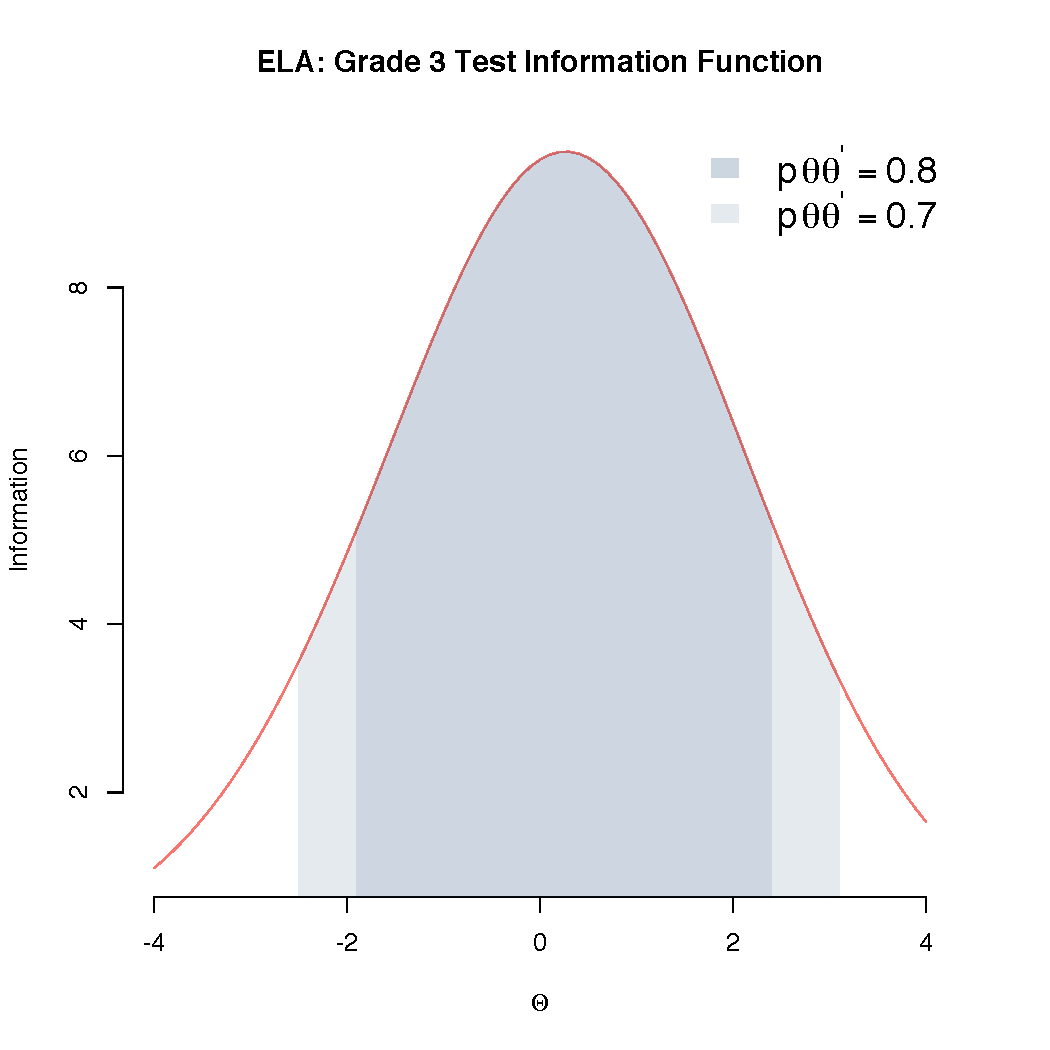
\includegraphics[width=\textwidth,height=3.125in]{tifs/ela3tif.pdf}
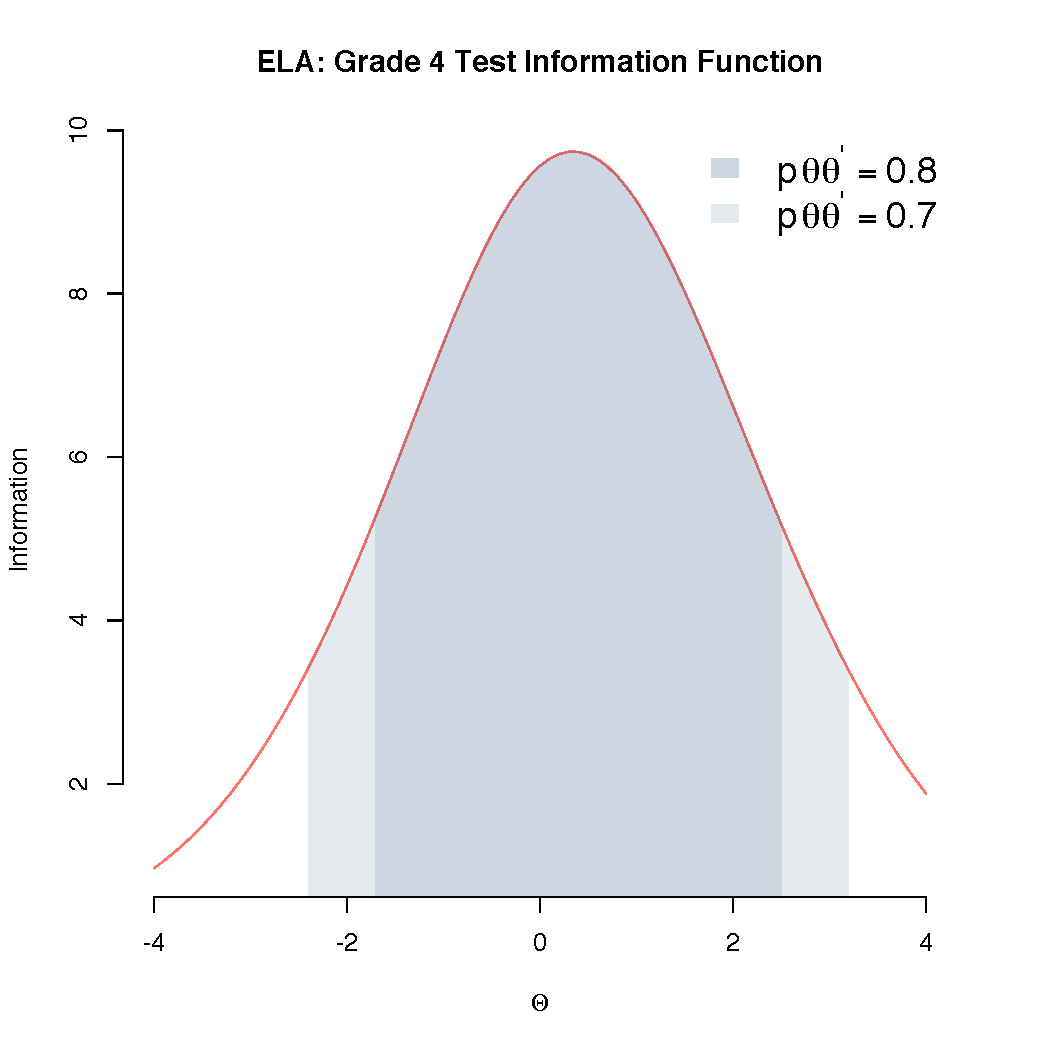
\includegraphics[width=\textwidth,height=3.125in]{tifs/ela4tif.pdf}
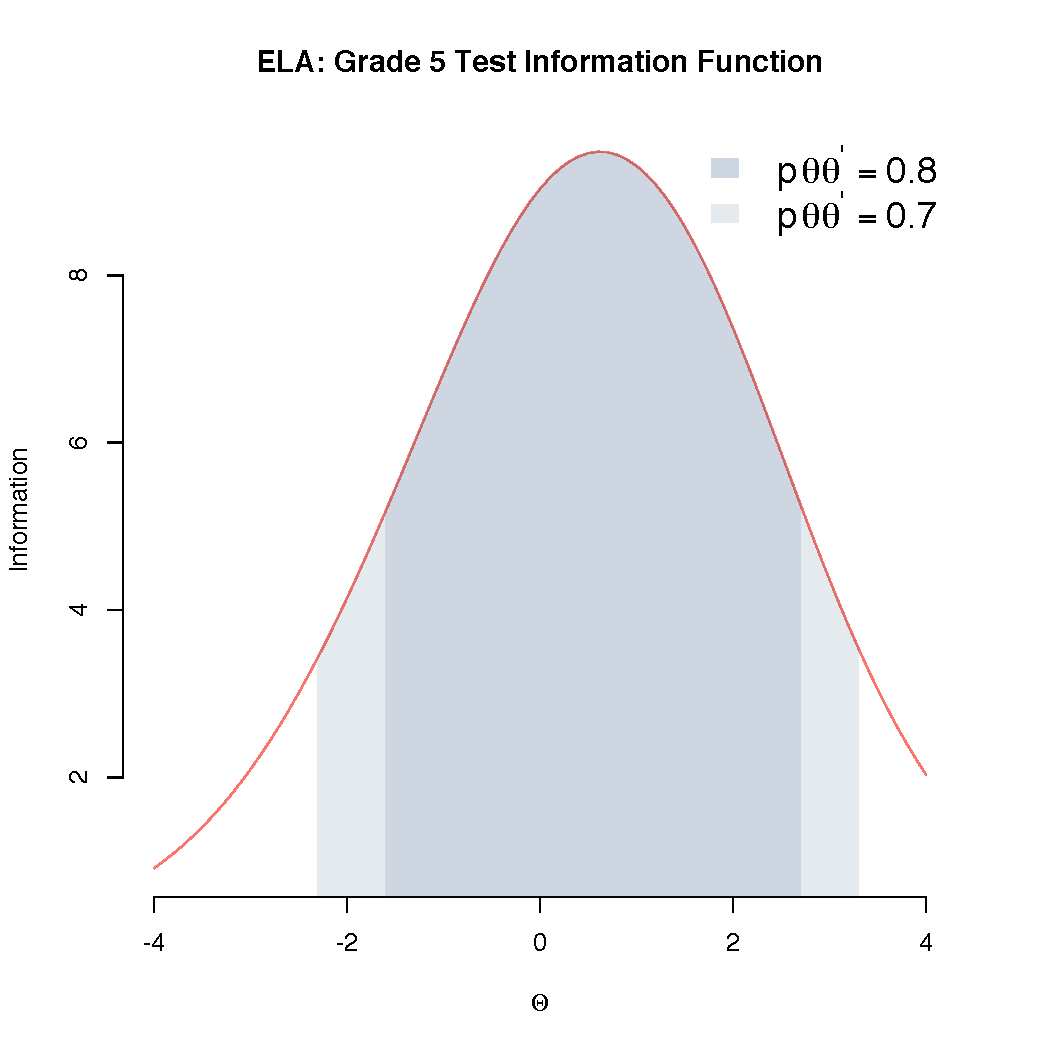
\includegraphics[width=\textwidth,height=3.125in]{tifs/ela5tif.pdf}
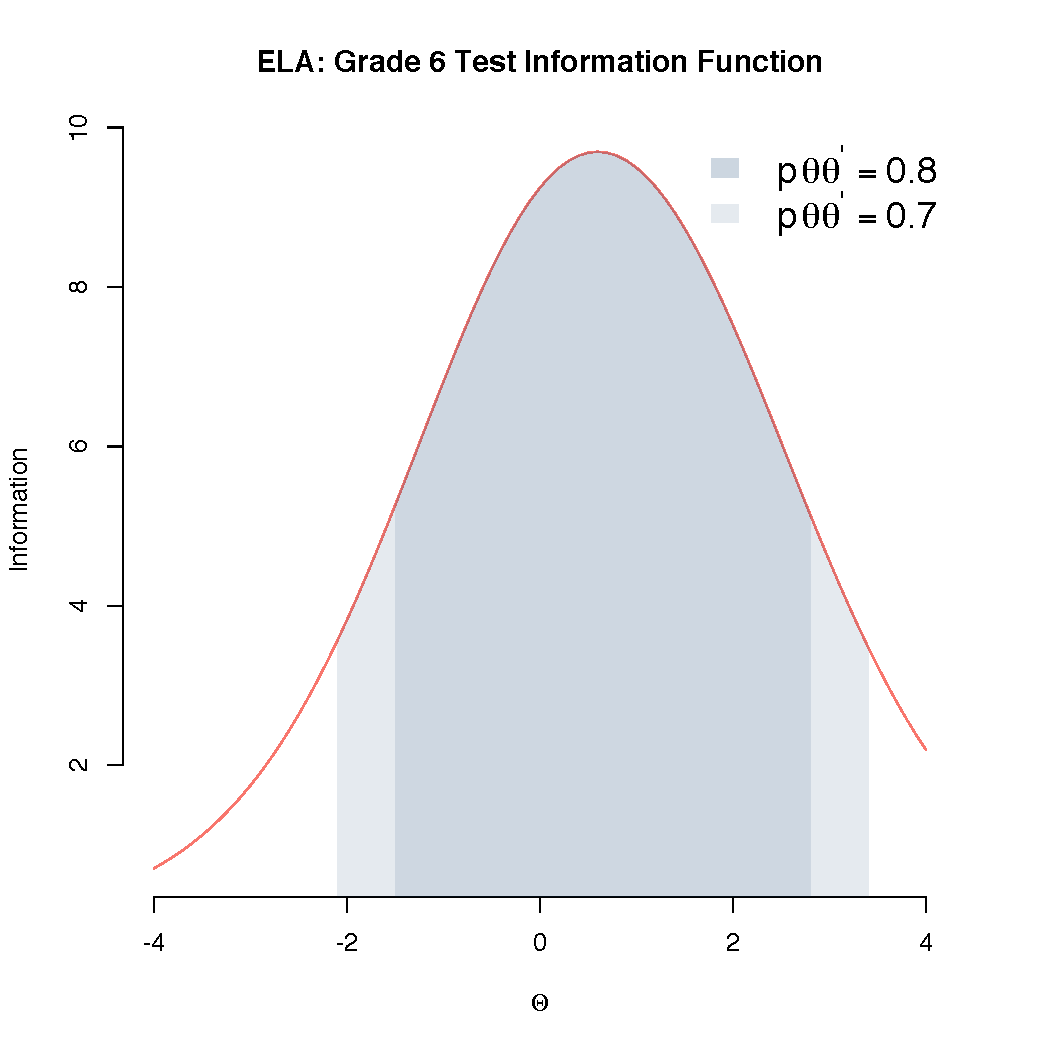
\includegraphics[width=\textwidth,height=3.125in]{tifs/ela6tif.pdf}
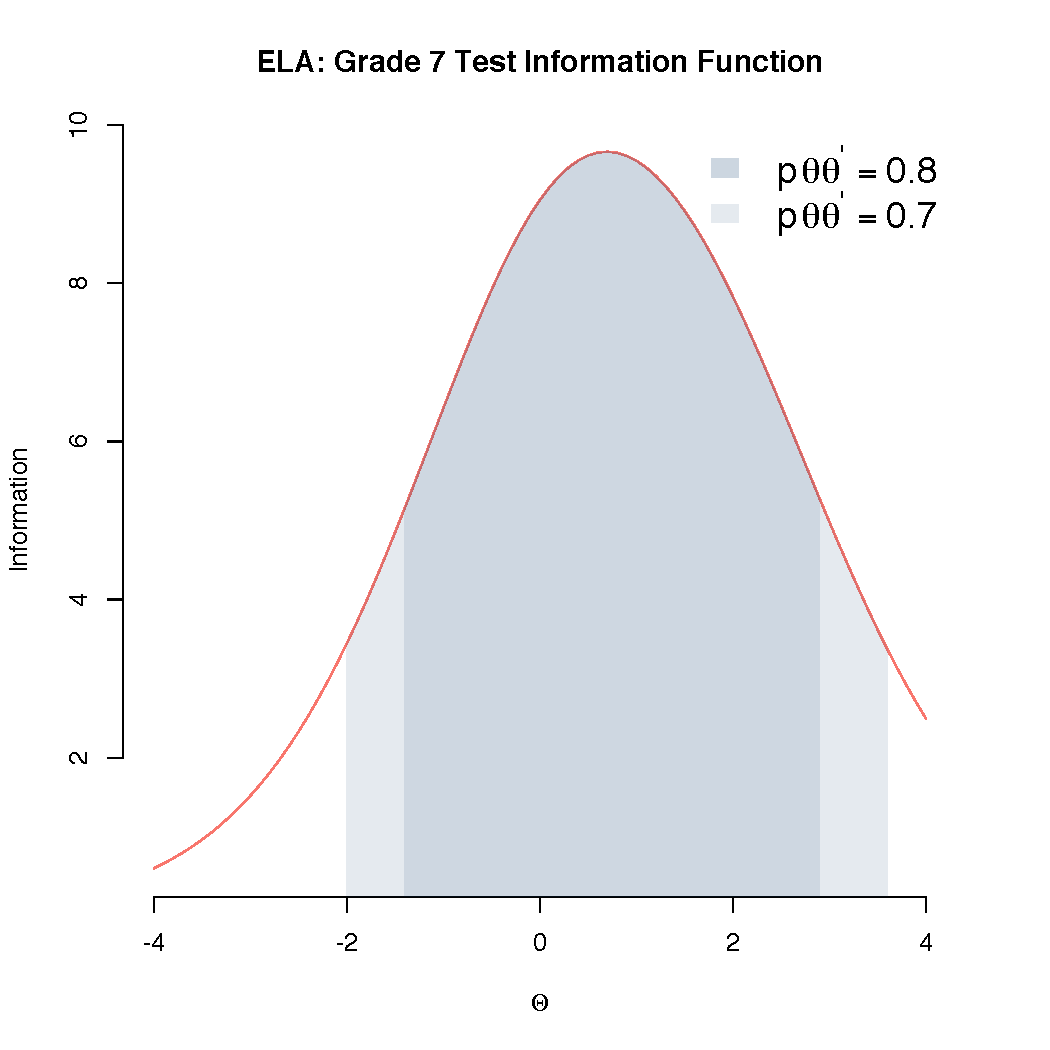
\includegraphics[width=\textwidth,height=3.125in]{tifs/ela7tif.pdf}
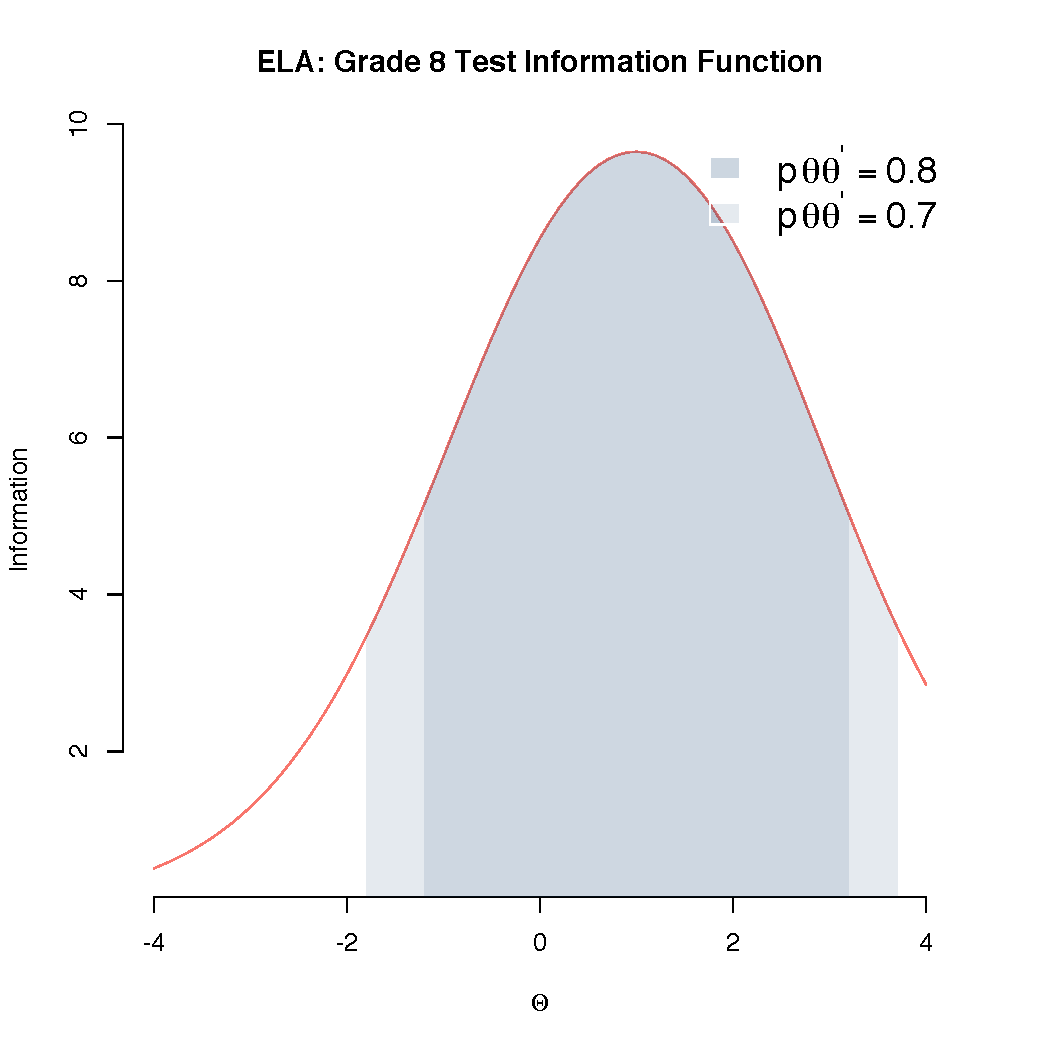
\includegraphics[width=\textwidth,height=3.125in]{tifs/ela8tif.pdf}
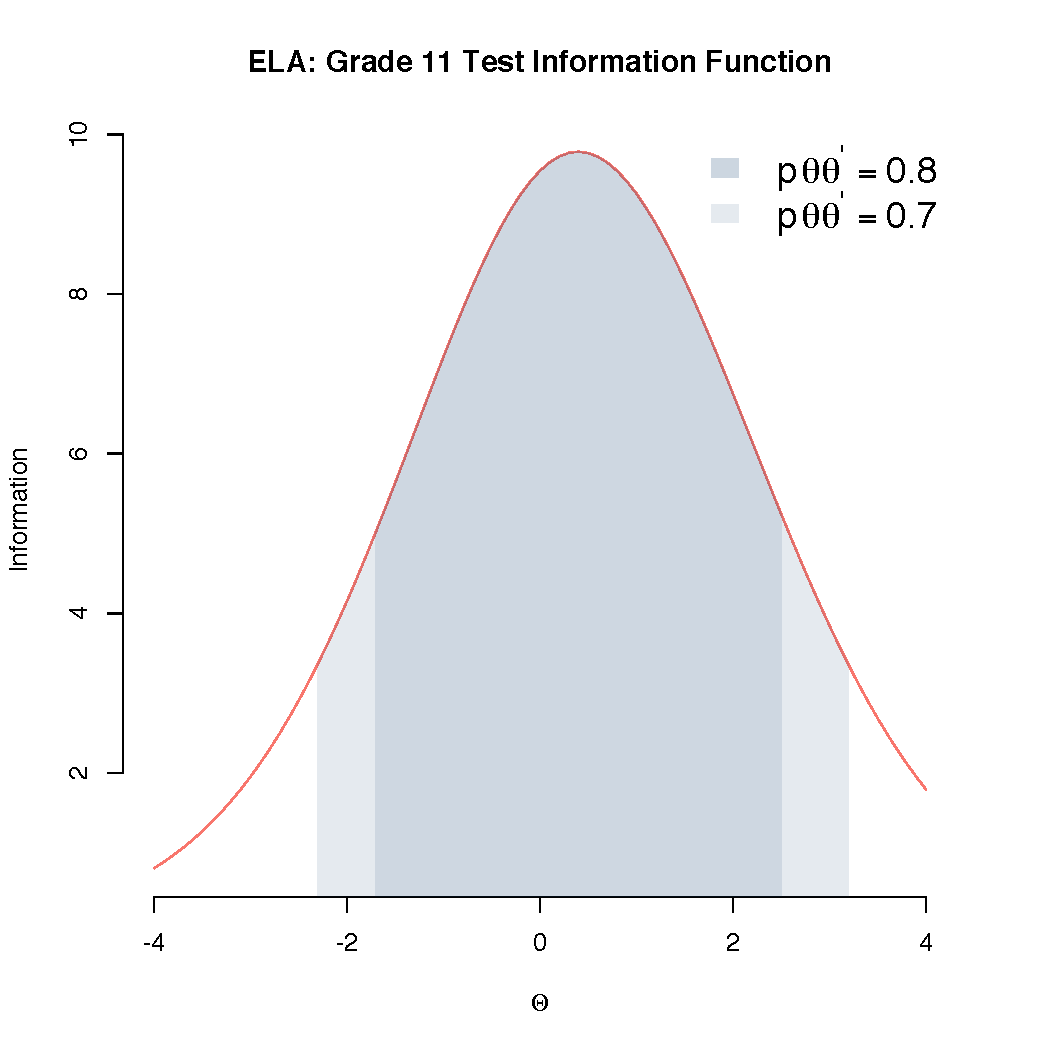
\includegraphics[width=\textwidth,height=3.125in]{tifs/ela11tif.pdf}
\newpage

\hypertarget{mathematics-tifs}{%
\paragraph{Mathematics TIFs}\label{mathematics-tifs}}

\FloatBarrier

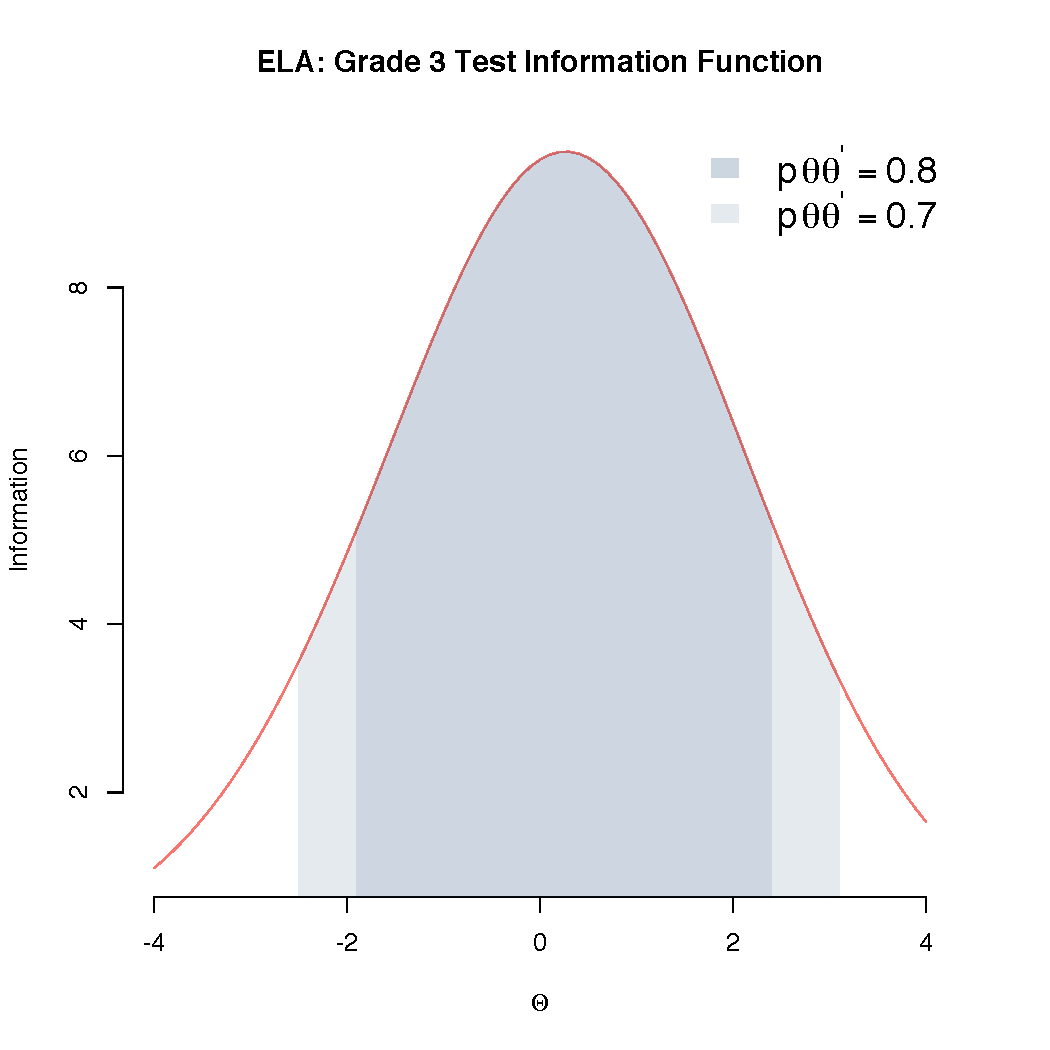
\includegraphics[width=\textwidth,height=3.125in]{tifs/ela3tif.pdf}
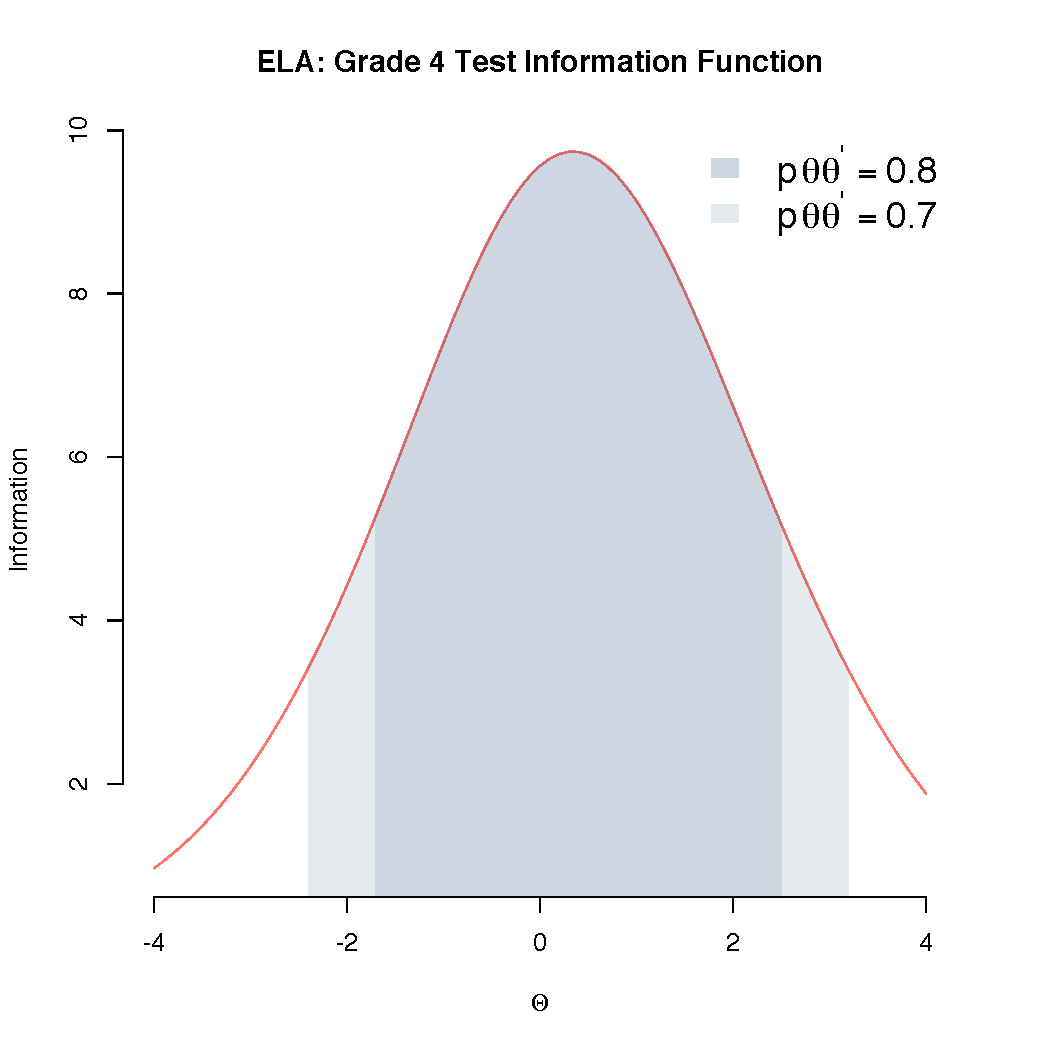
\includegraphics[width=\textwidth,height=3.125in]{tifs/ela4tif.pdf}
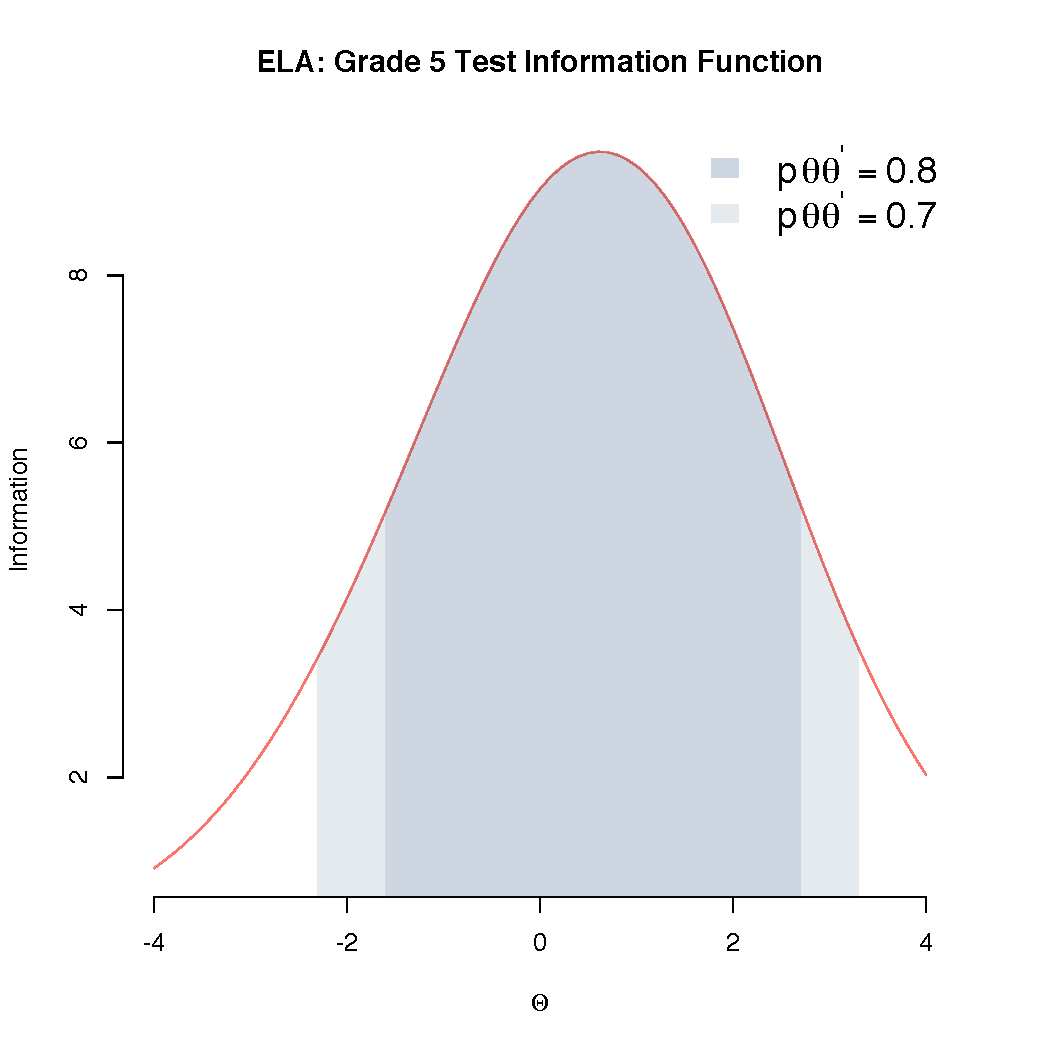
\includegraphics[width=\textwidth,height=3.125in]{tifs/ela5tif.pdf}
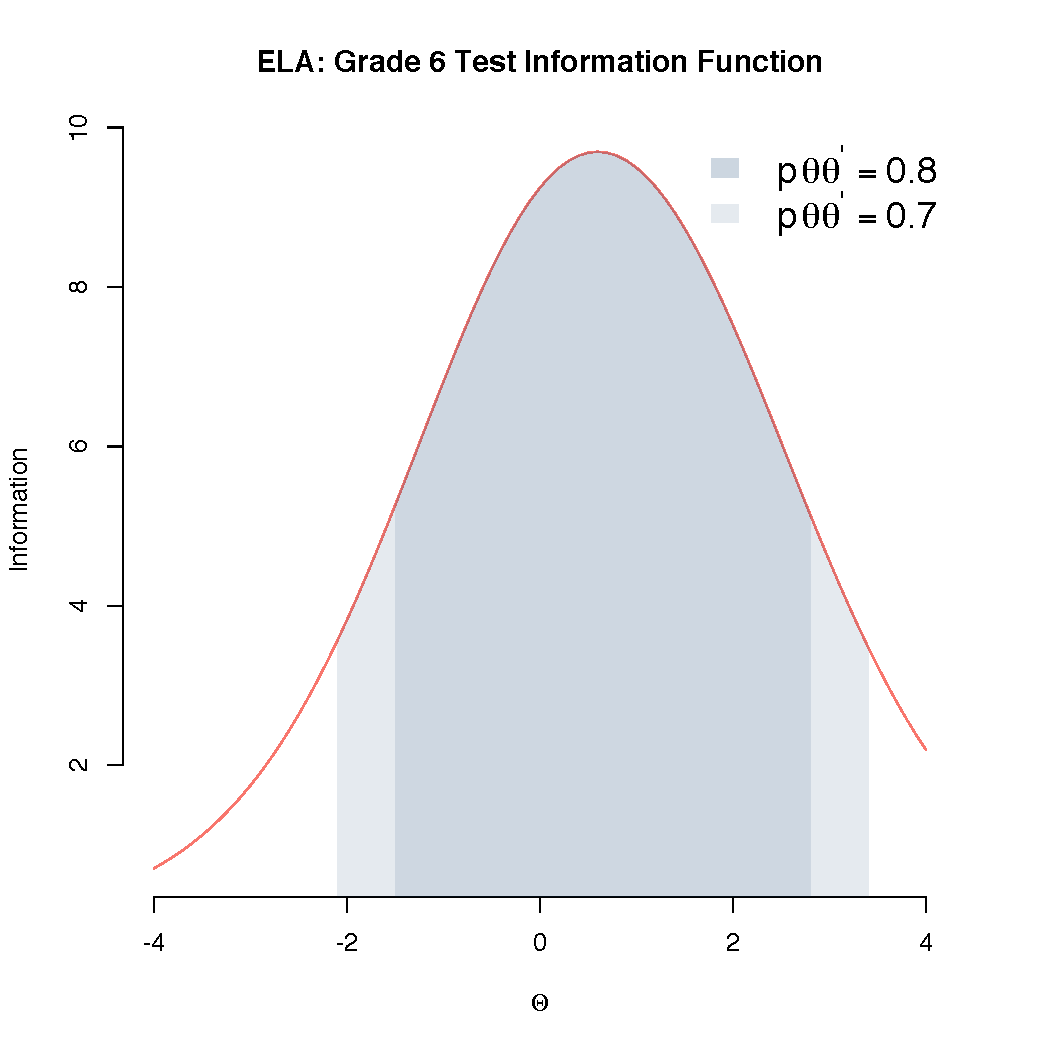
\includegraphics[width=\textwidth,height=3.125in]{tifs/ela6tif.pdf}
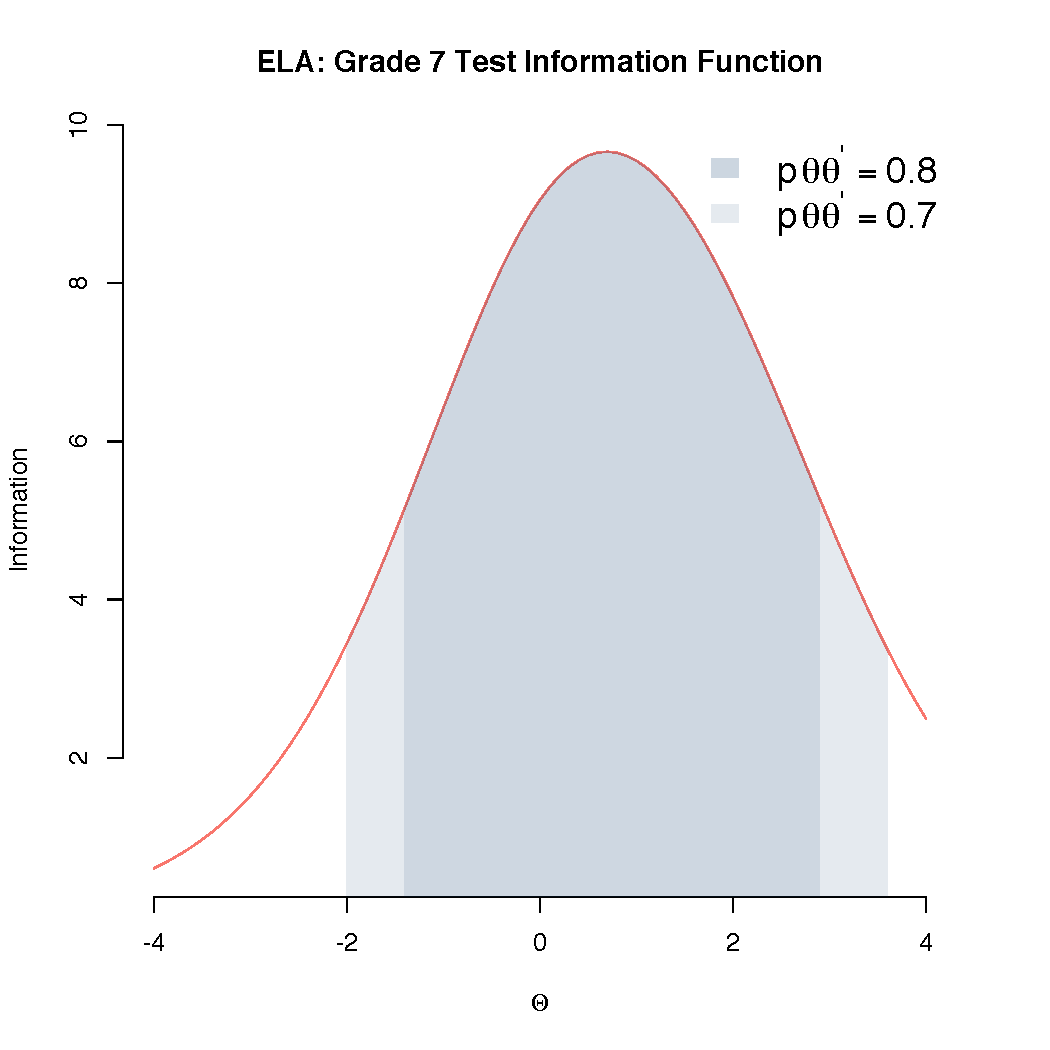
\includegraphics[width=\textwidth,height=3.125in]{tifs/ela7tif.pdf}
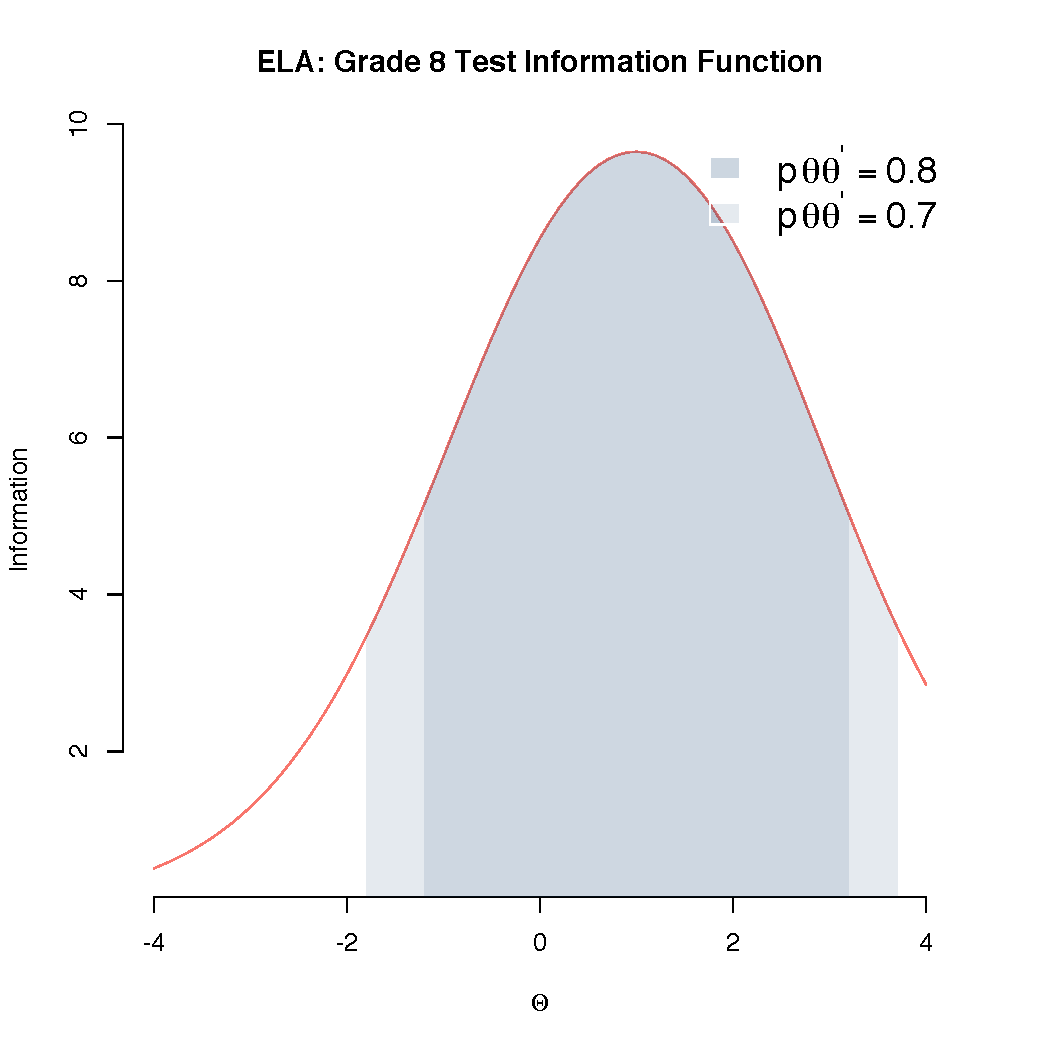
\includegraphics[width=\textwidth,height=3.125in]{tifs/ela8tif.pdf}
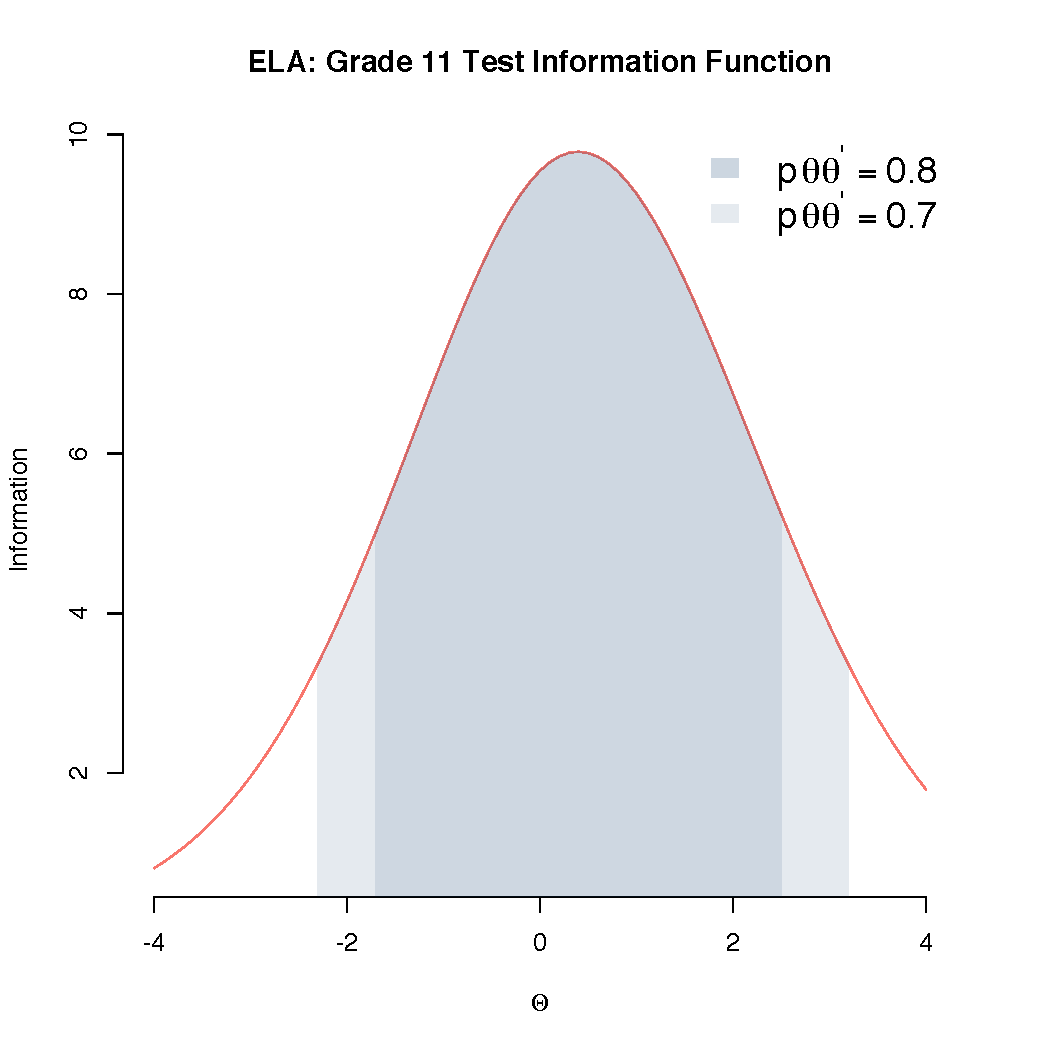
\includegraphics[width=\textwidth,height=3.125in]{tifs/ela11tif.pdf}
\newpage

\hypertarget{science-tifs}{%
\paragraph{Science TIFs}\label{science-tifs}}

\FloatBarrier

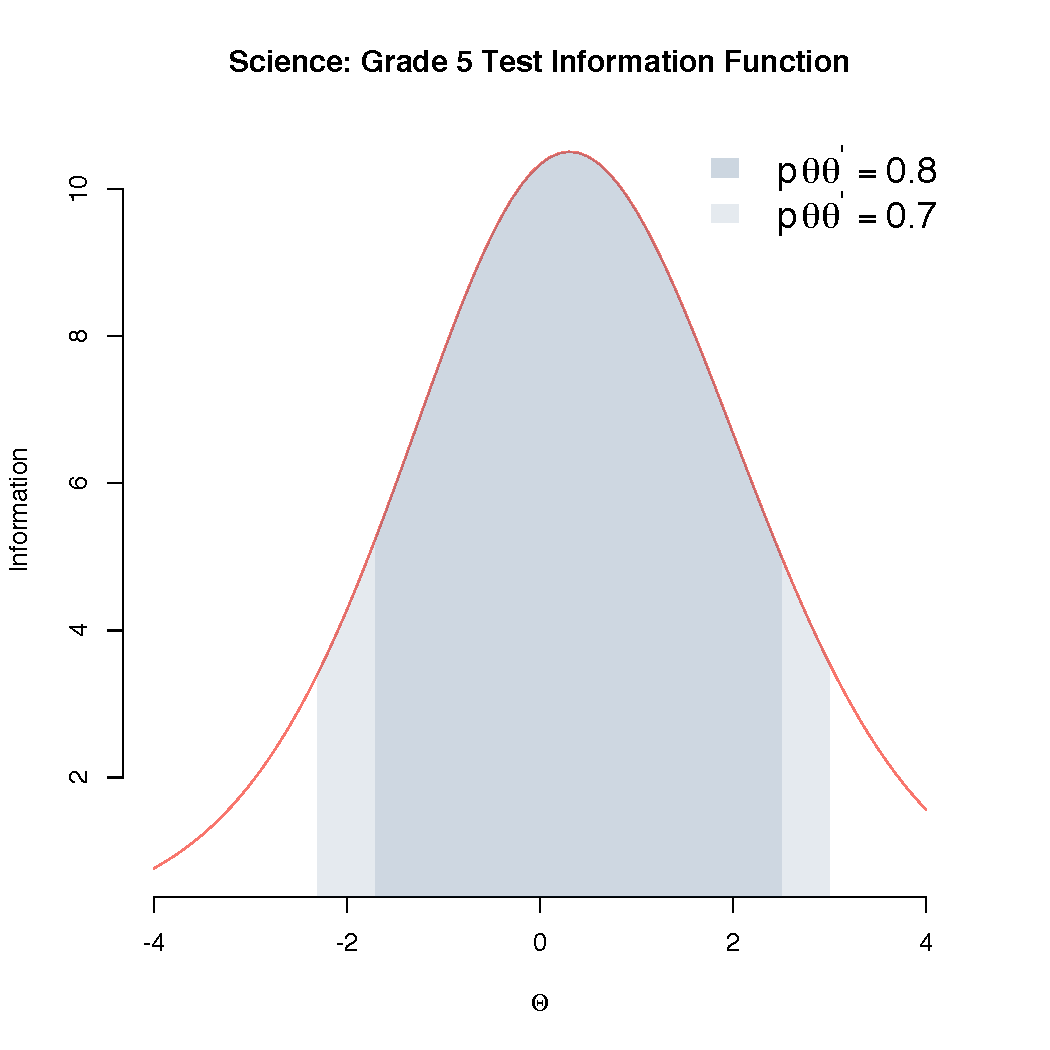
\includegraphics[width=\textwidth,height=3.125in]{tifs/science5tif.pdf}
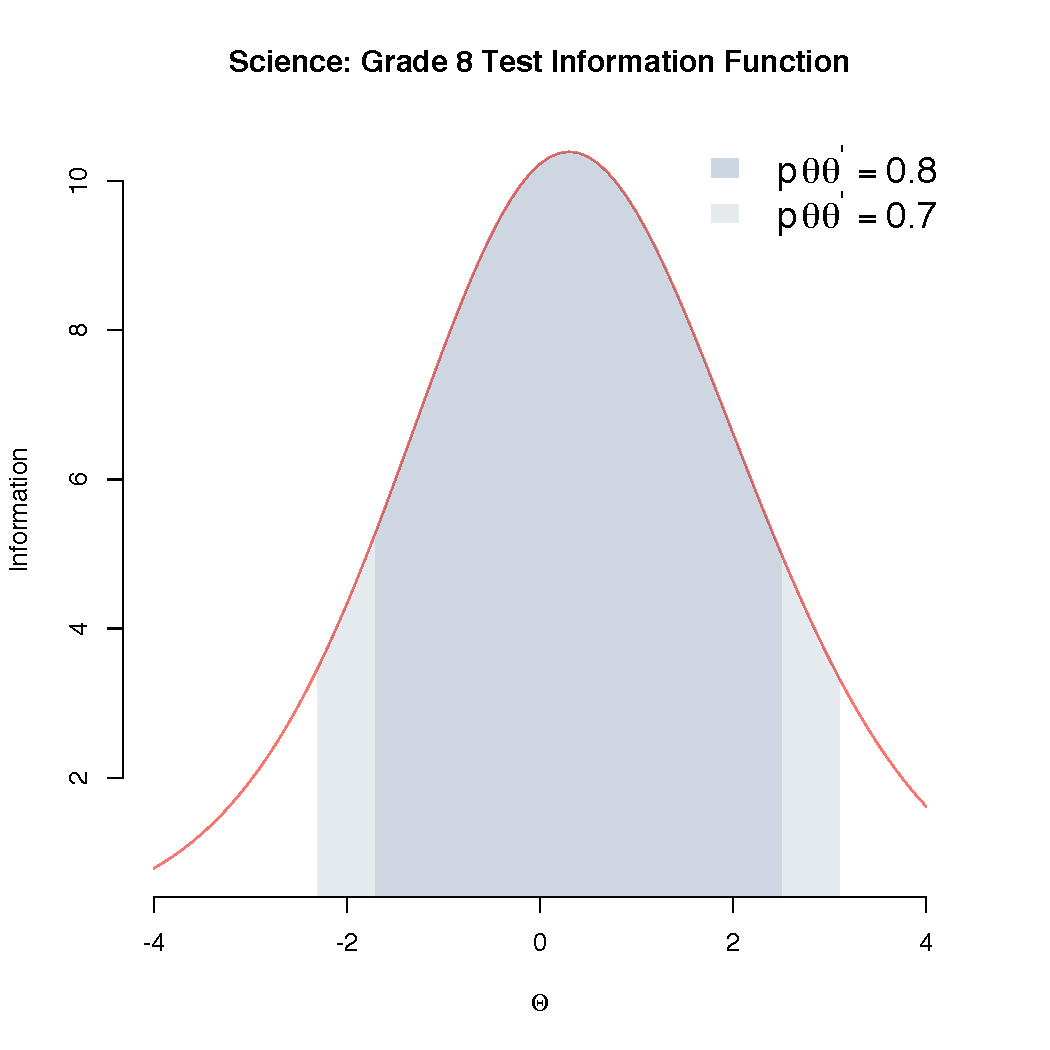
\includegraphics[width=\textwidth,height=3.125in]{tifs/science8tif.pdf}
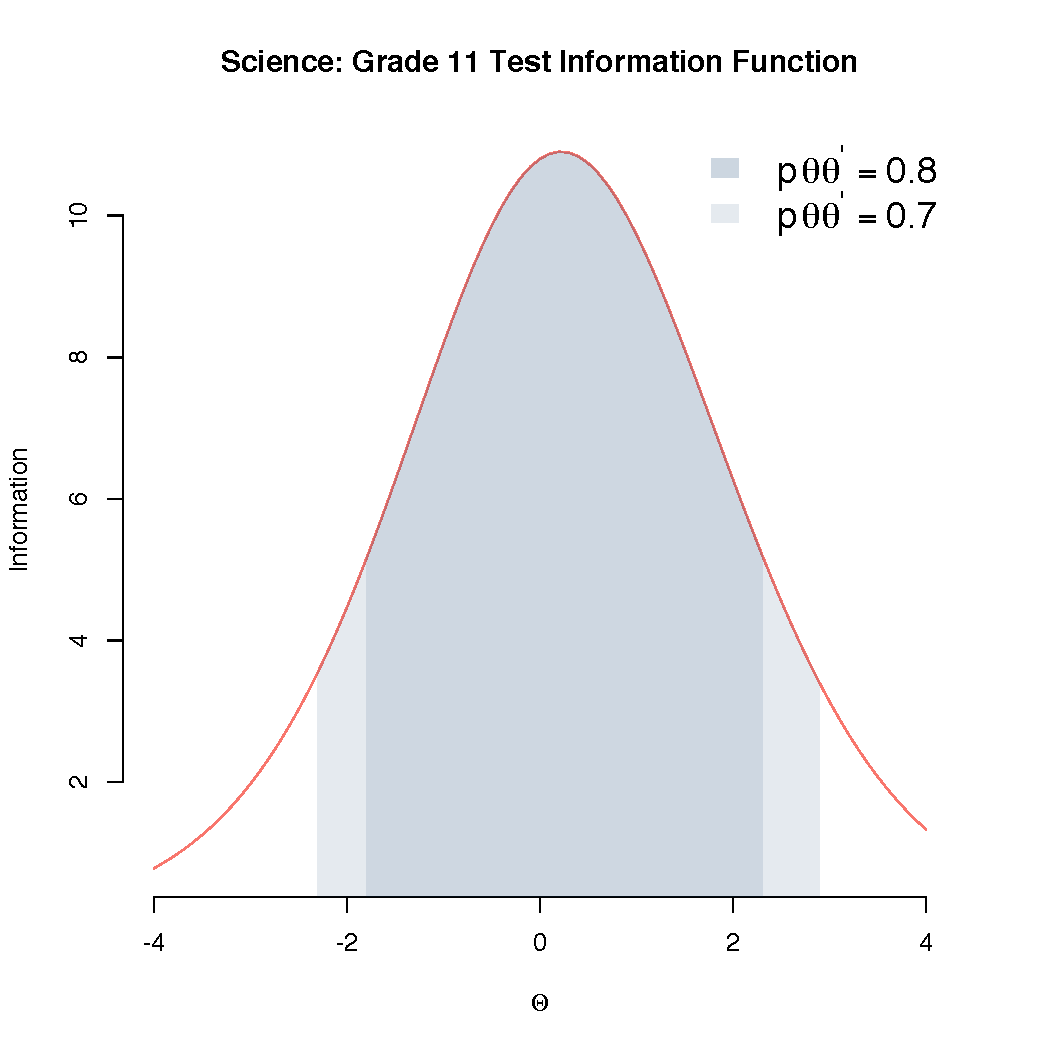
\includegraphics[width=\textwidth,height=3.125in]{tifs/science11tif.pdf}

\hypertarget{validation-of-orext-vertical-scales}{%
\paragraph{Validation of ORExt Vertical
Scales}\label{validation-of-orext-vertical-scales}}

The test characteristic curves (TCCs) for the grade-level assessments in
ELA and mathematics demonstrate incrementally increasing growth and test
demands across Grades 3-8, with the exception of Grade 7 mathematics.
The Grade 7 mathematics assessment was revised to be more difficult last
year, but clearly more elaboration of this effort is needed to address
its location on the TCC. Grade 11 and science tests are not vertically
scaled; TCCs are thus not presented for Grade 11 or science. All Rasch
model scaling, as well as the data visualizations for the TCCs were
conducted in the R software 3.3.2 environment (R Core Team, 2016) using
the r2Winsteps package (Anderson, 2015). \FloatBarrier
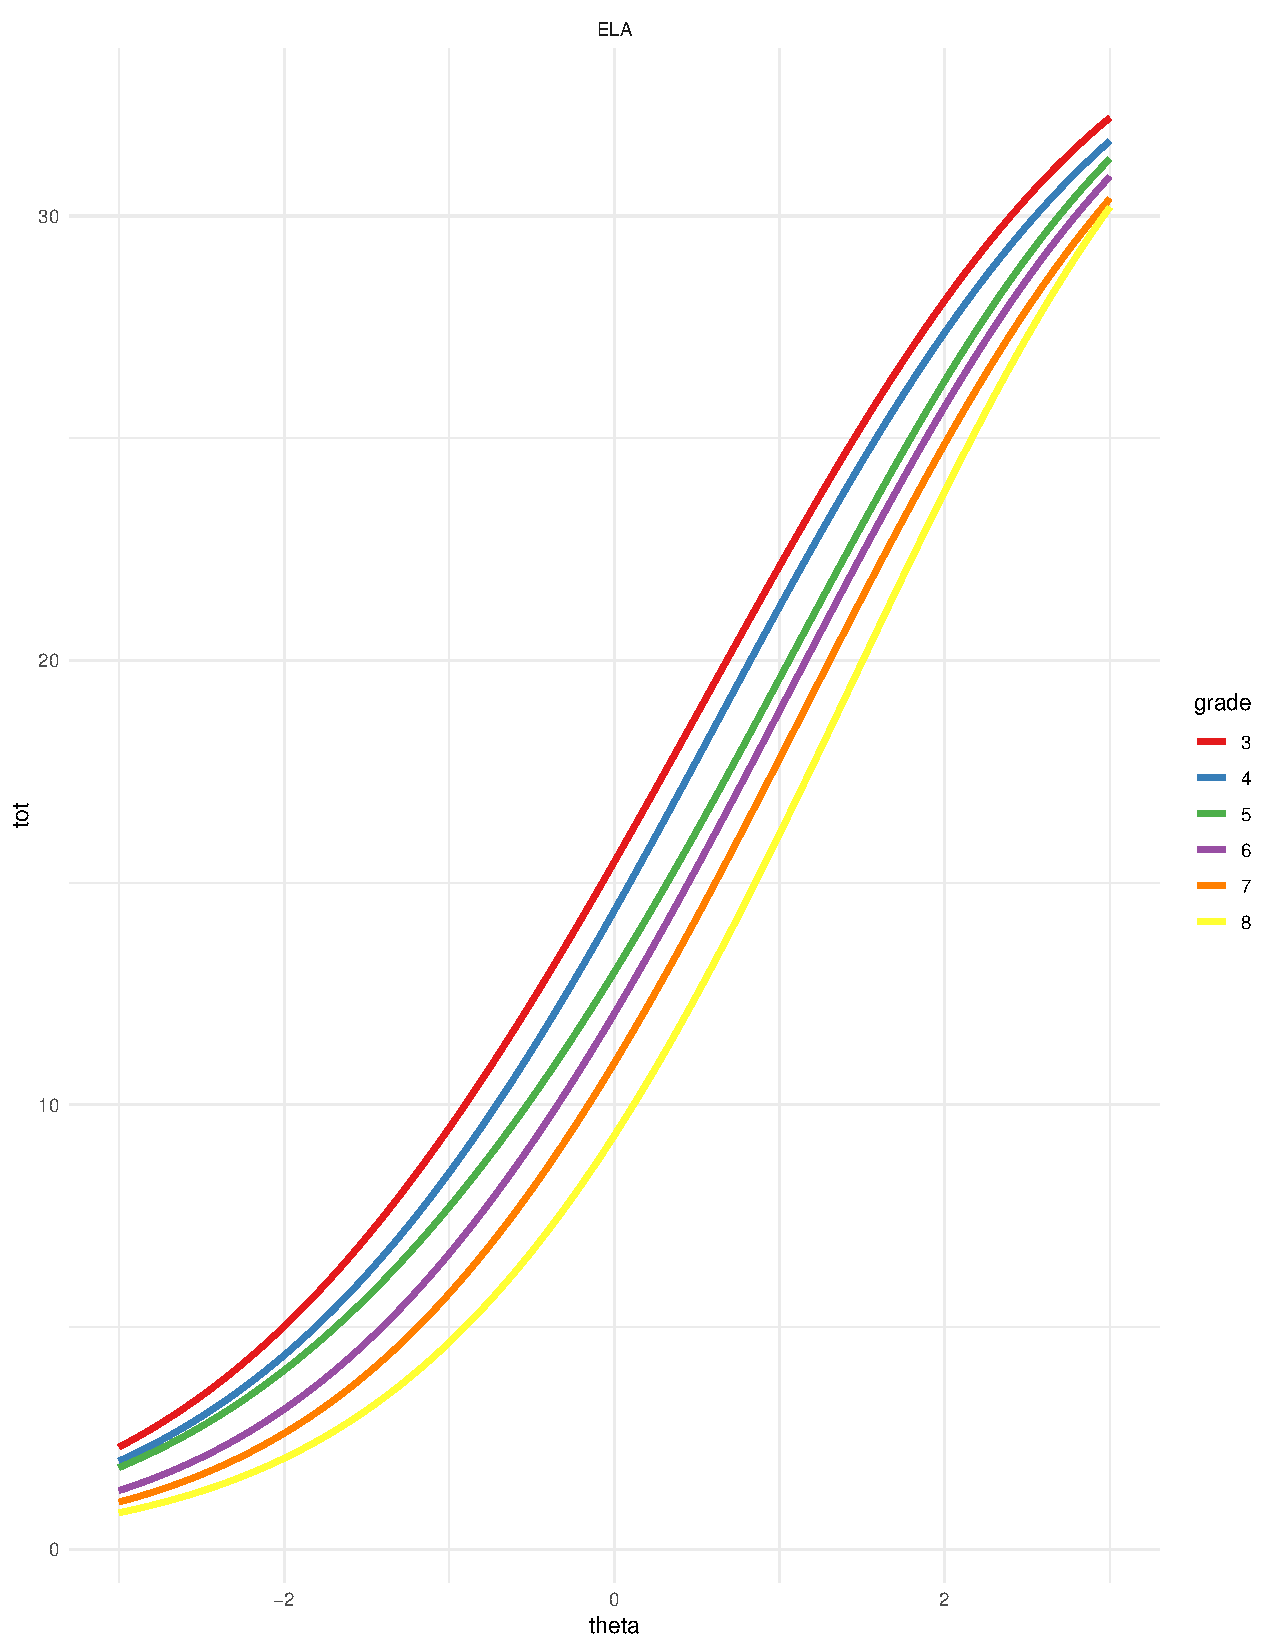
\includegraphics{tccs/019ELA_TCC.pdf}
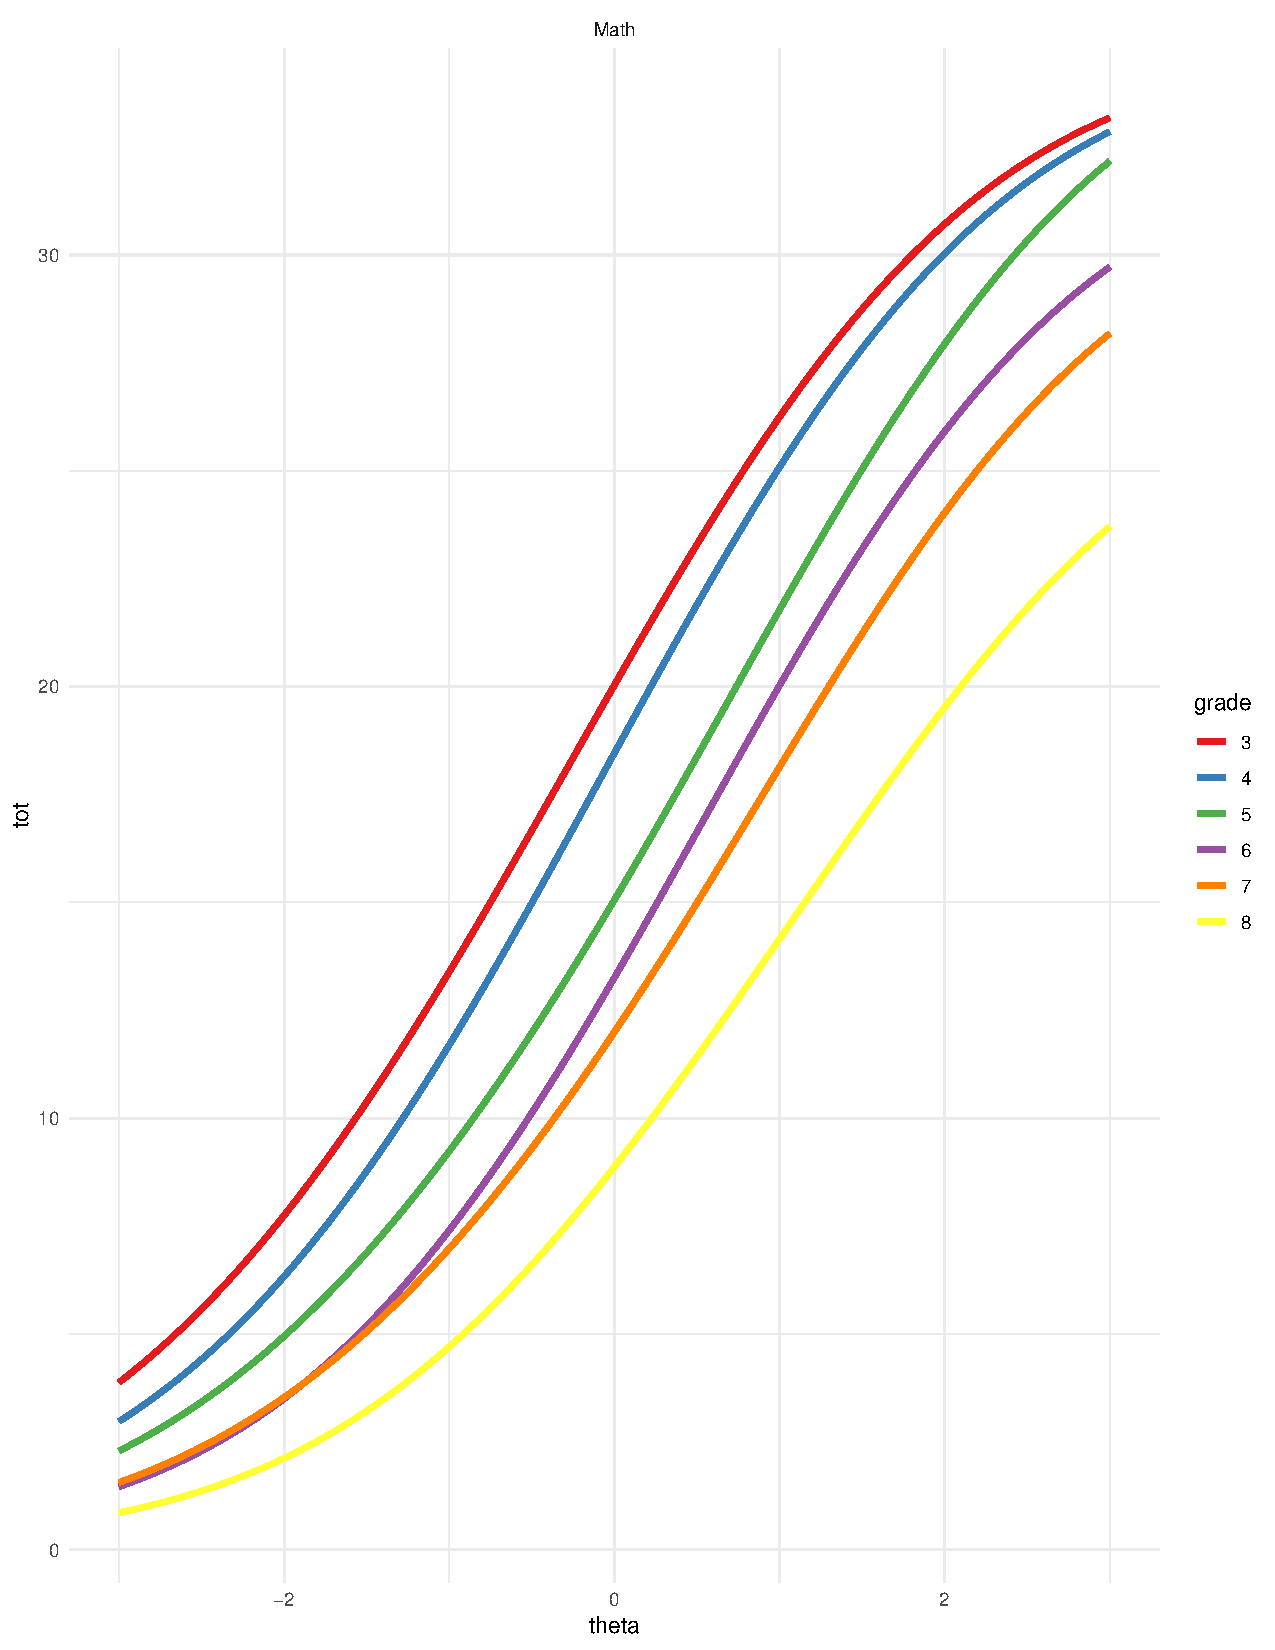
\includegraphics{tccs/019MathTCC.pdf} \clearpage

\hypertarget{b-overall-and-conditional-standard-errors-of-measure}{%
\paragraph{4.1B Overall and Conditional Standard Errors of
Measure}\label{b-overall-and-conditional-standard-errors-of-measure}}

The average SEM associated with each cut score for 2017-18 student data
are presented in the table below, supported by a KEY. The SEMs decreased
in almost all cases compared to last year, suggesting that the measures
are more reliable when student eligibility is more strictly controlled.
See Section 4.2 below for means and standard deviations by grade and
subject area. SEM = Standard Error of Measure associated with the cut
score to the left; averaged to the tenths' place. Level 1 = Does Not Yet
Meet (not included as the lowest level of proficiency) Level 2 = Nearly
Meets Level 3 = Meets Level 4 = Exceeds

\FloatBarrier

\begin{Shaded}
\begin{Highlighting}[]
\NormalTok{se_tbls <-}\StringTok{ }\NormalTok{ode }\OperatorTok\StringTok{ }
\StringTok{  }\KeywordTok{filter}\NormalTok{(content_area }\OperatorTok{==}\StringTok{ "ela"} \OperatorTok{|}
\StringTok{         }\NormalTok{content_area }\OperatorTok{==}\StringTok{ "math"} \OperatorTok{|}
\StringTok{         }\NormalTok{content_area }\OperatorTok{==}\StringTok{ "sci"}\NormalTok{) }\OperatorTok\StringTok{ }
\StringTok{  }\KeywordTok{group_by}\NormalTok{(content_area, grade, amo_lvl) }\OperatorTok\StringTok{ }
\StringTok{  }\NormalTok{sundry}\OperatorTok{::}\KeywordTok{filter_by_funs}\NormalTok{(rit, min) }\OperatorTok\StringTok{ }
\StringTok{  }\KeywordTok{select}\NormalTok{(content_area, grade, amo_lvl, rit, rit_se) }\OperatorTok\StringTok{ }
\StringTok{  }\KeywordTok{distinct}\NormalTok{() }\OperatorTok\StringTok{ }
\StringTok{  }\KeywordTok{arrange}\NormalTok{(content_area, grade, amo_lvl) }\OperatorTok\StringTok{ }
\StringTok{  }\KeywordTok{filter}\NormalTok{(amo_lvl }\OperatorTok{>}\StringTok{ }\DecValTok{1}\NormalTok{) }\OperatorTok\StringTok{ }
\StringTok{  }\KeywordTok{rename}\NormalTok{(}\DataTypeTok{Grade =}\NormalTok{ grade,}
         \DataTypeTok{AMO   =}\NormalTok{ amo_lvl, }
         \DataTypeTok{RIT   =}\NormalTok{ rit, }
         \DataTypeTok{SE    =}\NormalTok{ rit_se) }\OperatorTok\StringTok{ }
\StringTok{  }\KeywordTok{split}\NormalTok{(.}\OperatorTok{$}\NormalTok{content_area) }\OperatorTok\StringTok{ }
\StringTok{  }\KeywordTok{map}\NormalTok{(}\OperatorTok{~}\KeywordTok{ungroup}\NormalTok{(.) }\OperatorTok\StringTok{ }\KeywordTok{select}\NormalTok{(}\OperatorTok{-}\NormalTok{content_area))}

\KeywordTok{walk2}\NormalTok{(se_tbls,}
      \KeywordTok{paste0}\NormalTok{(}\KeywordTok{c}\NormalTok{(}\StringTok{"ELA"}\NormalTok{, }\StringTok{"Math"}\NormalTok{, }\StringTok{"Science"}\NormalTok{),}
             \StringTok{" Cut Score Standard Errors"}\NormalTok{), }
      \OperatorTok{~}\NormalTok{knitr}\OperatorTok{::}\KeywordTok{kable}\NormalTok{(.x, }\StringTok{"latex"}\NormalTok{, }\DataTypeTok{booktabs =} \OtherTok{TRUE}\NormalTok{,}
                     \DataTypeTok{caption =}\NormalTok{ .y,}
                    \DataTypeTok{digits =} \DecValTok{2}\NormalTok{) }\OperatorTok\StringTok{ }
\StringTok{        }\KeywordTok{kable_styling}\NormalTok{(}\DataTypeTok{full_width =} \OtherTok{TRUE}\NormalTok{,}
                      \DataTypeTok{latex_options =} \StringTok{"hold_position"}\NormalTok{) }\OperatorTok\StringTok{ }
\StringTok{        }\KeywordTok{print}\NormalTok{())}
\end{Highlighting}
\end{Shaded}

\FloatBarrier

\hypertarget{c-classification-accuracy-consistency}{%
\paragraph{4.1C Classification Accuracy \&
Consistency}\label{c-classification-accuracy-consistency}}

Results from the 2017-18 ORExt test administration were analyzed using
Rudner's classification index (Rudner, 2005). Results closer to 1.0
indicate the likelihood that a student was appropriately classified as
proficient or not proficient (accuracy) and the likelihood that the
student would be classified in the same category given an additional
test administration. The calculation utilizes item difficulty and theta
value distributions, as well as related standard errors of measurement,
to generate probabilistic estimates based on one test administration.
Complete results, generated from the cacIRT package in R, are provided
below. Results denote very high levels of classification accuracy and
consistency.

\FloatBarrier

\begin{Shaded}
\begin{Highlighting}[]
\NormalTok{cuts <-}\StringTok{ }\NormalTok{ode }\OperatorTok\StringTok{ }
\StringTok{  }\KeywordTok{group_by}\NormalTok{(content_area, grade, amo_lvl) }\OperatorTok\StringTok{ }
\StringTok{  }\KeywordTok{summarize}\NormalTok{(}\DataTypeTok{cut =} \KeywordTok{min}\NormalTok{(theta)) }\OperatorTok\StringTok{ }
\StringTok{  }\KeywordTok{filter}\NormalTok{(amo_lvl }\OperatorTok{>}\StringTok{ }\DecValTok{1}\NormalTok{)}

\NormalTok{diffs <-}\StringTok{ }\KeywordTok{map_df}\NormalTok{(}\KeywordTok{dir_ls}\NormalTok{(}\KeywordTok{file.path}\NormalTok{(}\StringTok{"data"}\NormalTok{, }\StringTok{"ifiles18"}\NormalTok{)), read_sub_files)}

\NormalTok{cuts <-}\StringTok{ }\NormalTok{diffs }\OperatorTok\StringTok{ }
\StringTok{  }\KeywordTok{select}\NormalTok{(content_area, grade, difficulty) }\OperatorTok\StringTok{ }
\StringTok{  }\KeywordTok{nest}\NormalTok{(}\OperatorTok{-}\NormalTok{content_area, }\OperatorTok{-}\NormalTok{grade) }\OperatorTok\StringTok{ }
\StringTok{  }\KeywordTok{mutate}\NormalTok{(}\DataTypeTok{ip =} \KeywordTok{map}\NormalTok{(data, }\OperatorTok{~}\KeywordTok{as.matrix}\NormalTok{(}\KeywordTok{data.frame}\NormalTok{(}\DecValTok{1}\NormalTok{, .}\OperatorTok{$}\NormalTok{difficulty, }\DecValTok{0}\NormalTok{))),}
         \DataTypeTok{content_area =} \KeywordTok{tolower}\NormalTok{(content_area)) }\OperatorTok\StringTok{ }
\StringTok{  }\KeywordTok{left_join}\NormalTok{(cuts)}

\NormalTok{abils <-}\StringTok{ }\NormalTok{ode }\OperatorTok\StringTok{ }
\StringTok{  }\KeywordTok{nest}\NormalTok{(}\OperatorTok{-}\NormalTok{content_area, }\OperatorTok{-}\NormalTok{grade) }\OperatorTok\StringTok{ }
\StringTok{  }\KeywordTok{rename}\NormalTok{(}\DataTypeTok{persons =}\NormalTok{ data)}

\NormalTok{cuts <-}\StringTok{ }\KeywordTok{left_join}\NormalTok{(cuts, abils)}

\NormalTok{acc_con_tbls <-}\StringTok{ }\NormalTok{cuts }\OperatorTok\StringTok{ }
\StringTok{  }\KeywordTok{mutate}\NormalTok{(}\DataTypeTok{theta =} \KeywordTok{map}\NormalTok{(persons, }\StringTok{"theta"}\NormalTok{),}
         \DataTypeTok{se    =} \KeywordTok{map}\NormalTok{(persons, }\StringTok{"se"}\NormalTok{),}
         \DataTypeTok{marginal =} \KeywordTok{pmap}\NormalTok{(}\KeywordTok{list}\NormalTok{(cut, ip, theta, se), }
                         \ControlFlowTok{function}\NormalTok{(cut, ip, theta, se)}
                         \KeywordTok{class.Rud}\NormalTok{(cut, ip, theta, se, }\DataTypeTok{D =} \DecValTok{1}\NormalTok{)}\OperatorTok{$}\NormalTok{Marginal),}
         \DataTypeTok{accuracy =} \KeywordTok{map_dbl}\NormalTok{(marginal, }\DecValTok{1}\NormalTok{),}
         \DataTypeTok{consistency =} \KeywordTok{map_dbl}\NormalTok{(marginal, }\DecValTok{2}\NormalTok{)) }\OperatorTok\StringTok{ }
\StringTok{  }\KeywordTok{select}\NormalTok{(content_area, grade, amo_lvl, accuracy, consistency) }\OperatorTok\StringTok{ }
\StringTok{  }\KeywordTok{rename}\NormalTok{(}\DataTypeTok{Grade =}\NormalTok{ grade,}
         \DataTypeTok{AMO   =}\NormalTok{ amo_lvl,}
         \DataTypeTok{Accuracy =}\NormalTok{ accuracy,}
         \DataTypeTok{Consistency =}\NormalTok{ consistency) }\OperatorTok\StringTok{ }
\StringTok{  }\KeywordTok{split}\NormalTok{(.}\OperatorTok{$}\NormalTok{content_area) }\OperatorTok\StringTok{ }
\StringTok{  }\KeywordTok{map}\NormalTok{(}\OperatorTok{~}\KeywordTok{ungroup}\NormalTok{(.) }\OperatorTok\StringTok{ }\KeywordTok{select}\NormalTok{(}\OperatorTok{-}\NormalTok{content_area))}

\KeywordTok{walk2}\NormalTok{(acc_con_tbls,}
      \KeywordTok{paste0}\NormalTok{(}\KeywordTok{c}\NormalTok{(}\StringTok{"ELA"}\NormalTok{, }\StringTok{"Math"}\NormalTok{, }\StringTok{"Science"}\NormalTok{),}
             \StringTok{" Accuracy/Consistency"}\NormalTok{), }
      \OperatorTok{~}\NormalTok{knitr}\OperatorTok{::}\KeywordTok{kable}\NormalTok{(.x, }\StringTok{"latex"}\NormalTok{, }\DataTypeTok{booktabs =} \OtherTok{TRUE}\NormalTok{,}
                     \DataTypeTok{caption =}\NormalTok{ .y,}
                    \DataTypeTok{digits =} \DecValTok{2}\NormalTok{) }\OperatorTok\StringTok{ }
\StringTok{        }\KeywordTok{kable_styling}\NormalTok{(}\DataTypeTok{full_width =} \OtherTok{TRUE}\NormalTok{,}
                      \DataTypeTok{latex_options =} \StringTok{"hold_position"}\NormalTok{) }\OperatorTok\StringTok{ }
\StringTok{        }\KeywordTok{print}\NormalTok{())}
\end{Highlighting}
\end{Shaded}

\FloatBarrier

The ORExt is not a computer-adaptive instrument so estimate precision
documentation based upon that test design is not provided.

\hypertarget{fairness-and-accessibility}{%
\subsubsection{4.2 Fairness and
Accessibility}\label{fairness-and-accessibility}}

The state has taken steps to ensure fairness in the development of the
assessments, including an analysis of each test item by Oregon teachers
not only for linkage to standards, but also for access, sensitivity, and
bias (see \emph{Appendix} 3.1A). In addition, we reviewed test
functioning as relevant to race/ethnicity and disability subgroups. This
process increases the likelihood that students are receiving instruction
in areas reflected in the assessment, and also that the items are not
biased toward a particular demographic or sub-group.

\hypertarget{differential-item-functioning-analyses}{%
\subparagraph{Differential Item Functioning
Analyses}\label{differential-item-functioning-analyses}}

To investigate Differential Item Functioning (DIF), the Mantel-Haenszel
test using a purification process was conducted (Holland \& Thayer,
1988; Kamata \& Vaughn, 2004) with the R software using the difR package
(Magis et al., 2013). When using the Mantel-Haenszel test to investigate
DIF, contingency tables are constructed, and the resulting odds for the
focal group answering the item correctly are compared to the odds for
the reference group. Given n-size limitations (Scott, et al., 2009), we
were able to conduct two analyses: a) White/Non-White and b)
Male/Female. Whites and Males were the focal groups and Non-Whites and
Females were the reference groups, respectively. The contingency table
summarizes correct and incorrect responses to each item by respondents'
total raw score by subgroup (Kamata \& Vaughn, 2004). If there is no
difference in performance for the two groups, the odds ratio of the
focal group performance to reference group performance will equal one.
An odds ratio greater than one means the focal group is performing
better than the reference group, with the opposite being true for odds
ratios less than one.

The difR package contains a built in algorithm to conduct purification
automatically, so we were interested in how this algorithm functioned
relative to the iterations conducted manually using SPSS. We used
criteria outlined by the Educational Testing Service (ETS) for DIF
Classification (Holland \& Thayer, 1988) to determine whether or not
items exhibited DIF, as the difR package reports delta values by
default, defined as \[\Delta_{MH} =
-2.35*ln(\alpha_{MH})\]

The Holland and Thayer criteria were used for all Mantel-Haenszel
analyses. Items that were flagged as ``C'' level items were reviewed by
BRT researchers for potential biases. If biases are identified, the item
is removed from the item pool. DIF analyses were performed ex post facto
on the 2015-16 ORExt operational items to address longitudinal trends.
Only three ELA items were identified as exhibiting a ``C'' level DIF
across both 2017 and 2018. Those three ELA items, one in Grade 5 that
exhibited DIF that privileged White examinees, one in Grade 4 that
privileged Female examinees, and one in Grade 8 that privileged Female
examinees, were removed and were not used in 2017-18 or thereafter. DIF
analyses was also be performed in the 2017-18 school year to continue to
address DIF longitudinally. All items, including field test items, were
included in the analyses. There are a total of 48 items on each
assessment.

Within the White/Non-White analysis, 10 out of 18 items flagged as ``C''
level items privileged Non-White test participants in ELA, 2 out of 5
privileged Non-White test participants in Mathematics, and 2 out of 7
privileged Non-White test participants in Science. Overall, DIF flagging
bases on race was relatively balanced, with 14 privileging students who
were Non-White and 16 privileging students who were White.

\FloatBarrier

\begin{Shaded}
\begin{Highlighting}[]
\NormalTok{raw <-}\StringTok{ }\KeywordTok{dir_ls}\NormalTok{(}\StringTok{"data/raw"}\NormalTok{, }\DataTypeTok{glob =} \StringTok{"*.txt"}\NormalTok{)}
\NormalTok{raw <-}\StringTok{ }\NormalTok{raw[}\OperatorTok{-}\KeywordTok{grep}\NormalTok{(}\StringTok{"XO"}\NormalTok{, raw)]}

\NormalTok{d <-}\StringTok{ }\KeywordTok{map_df}\NormalTok{(raw, read_delim, }\DataTypeTok{delim =} \StringTok{"|"}\NormalTok{, }\DataTypeTok{na =} \StringTok{"N"}\NormalTok{, }\DataTypeTok{.id =} \StringTok{"content"}\NormalTok{) }\OperatorTok
\StringTok{  }\KeywordTok{clean_names}\NormalTok{(}\StringTok{"old_janitor"}\NormalTok{) }\OperatorTok\StringTok{ }
\StringTok{  }\KeywordTok{mutate}\NormalTok{(}\DataTypeTok{content =} \KeywordTok{str_extract}\NormalTok{(content, }\StringTok{"XE|XM|XS"}\NormalTok{),}
         \DataTypeTok{content =} \KeywordTok{case_when}\NormalTok{(content }\OperatorTok{==}\StringTok{ "XE"} \OperatorTok{~}\StringTok{ "ELA"}\NormalTok{,}
\NormalTok{                             content }\OperatorTok{==}\StringTok{ "XM"} \OperatorTok{~}\StringTok{ "Math"}\NormalTok{,}
                             \OtherTok{TRUE} \OperatorTok{~}\StringTok{ "Science"}\NormalTok{),}
         \DataTypeTok{grade_for_match =} \KeywordTok{parse_number}\NormalTok{(enrlgrattst),}
         \DataTypeTok{grade_for_match =} \KeywordTok{ifelse}\NormalTok{(grade_for_match }\OperatorTok{==}\StringTok{ }\DecValTok{12}\NormalTok{, }
                                  \DecValTok{11}\NormalTok{, }
\NormalTok{                                  grade_for_match)) }\OperatorTok\StringTok{ }
\StringTok{  }\KeywordTok{gather}\NormalTok{(item, response, }\KeywordTok{starts_with}\NormalTok{(}\StringTok{"item"}\NormalTok{)) }\OperatorTok\StringTok{ }
\StringTok{  }\KeywordTok{mutate}\NormalTok{(}\DataTypeTok{item =} \KeywordTok{parse_number}\NormalTok{(item)) }

\NormalTok{item_ids <-}\StringTok{ }\KeywordTok{map_df}\NormalTok{(}\KeywordTok{dir_ls}\NormalTok{(}\StringTok{"data/tests"}\NormalTok{), }
                     \OperatorTok{~}\KeywordTok{read_csv}\NormalTok{(.) }\OperatorTok\StringTok{ }\KeywordTok{select}\NormalTok{(Item, }\StringTok{`}\DataTypeTok{Item ID}\StringTok{`}\NormalTok{), }
                     \DataTypeTok{.id =} \StringTok{"file"}\NormalTok{) }\OperatorTok\StringTok{ }
\StringTok{  }\NormalTok{janitor}\OperatorTok{::}\KeywordTok{clean_names}\NormalTok{() }\OperatorTok\StringTok{ }
\StringTok{  }\KeywordTok{mutate}\NormalTok{(}\DataTypeTok{content =} \KeywordTok{str_extract}\NormalTok{(file, }\StringTok{"ELA|Math|Science"}\NormalTok{),}
         \DataTypeTok{grade_for_match =} \KeywordTok{as.numeric}\NormalTok{(}\KeywordTok{gsub}\NormalTok{(}\StringTok{".+/G(}\CharTok{\textbackslash{}\textbackslash{}}\StringTok{d.?)(_.+)"}\NormalTok{, }\StringTok{"}\CharTok{\textbackslash{}\textbackslash{}}\StringTok{1"}\NormalTok{, file))) }\OperatorTok\StringTok{ }
\StringTok{  }\KeywordTok{select}\NormalTok{(}\OperatorTok{-}\NormalTok{file)}

\NormalTok{d <-}\StringTok{ }\KeywordTok{left_join}\NormalTok{(d, item_ids) }\OperatorTok\StringTok{ }
\StringTok{  }\KeywordTok{select}\NormalTok{(}\OperatorTok{-}\NormalTok{item) }\OperatorTok\StringTok{ }
\StringTok{  }\KeywordTok{group_by}\NormalTok{(grade_for_match, content) }\OperatorTok\StringTok{ }
\StringTok{  }\KeywordTok{nest}\NormalTok{() }\OperatorTok\StringTok{ }
\StringTok{  }\KeywordTok{mutate}\NormalTok{(}\DataTypeTok{data =} \KeywordTok{map}\NormalTok{(data, }\OperatorTok{~}\KeywordTok{spread}\NormalTok{(., item_id, response))) }\OperatorTok\StringTok{ }
\StringTok{  }\KeywordTok{mutate}\NormalTok{(}\DataTypeTok{data  =} \KeywordTok{map}\NormalTok{(data, }\OperatorTok{~}\KeywordTok{remove_empty}\NormalTok{(., }\StringTok{"cols"}\NormalTok{)),}
         \DataTypeTok{white =} \KeywordTok{map}\NormalTok{(data, }\OperatorTok{~}\KeywordTok{ifelse}\NormalTok{(.[[}\StringTok{"ethniccd"}\NormalTok{]] }\OperatorTok{==}\StringTok{ "W"}\NormalTok{, }\DecValTok{1}\NormalTok{, }\DecValTok{0}\NormalTok{)),}
         \DataTypeTok{male =} \KeywordTok{map}\NormalTok{(data, }\OperatorTok{~}\KeywordTok{ifelse}\NormalTok{(.[[}\StringTok{"gndr"}\NormalTok{]] }\OperatorTok{==}\StringTok{ "M"}\NormalTok{, }\DecValTok{1}\NormalTok{, }\DecValTok{0}\NormalTok{)),}
         \DataTypeTok{items =} \KeywordTok{map}\NormalTok{(data, }\OperatorTok{~}\KeywordTok{select}\NormalTok{(., }\OperatorTok{-}\NormalTok{testeventid}\OperatorTok{:-}\NormalTok{tstcmpltdt)),}
         \DataTypeTok{items =} \KeywordTok{map}\NormalTok{(items, }\OperatorTok{~}\KeywordTok{map_df}\NormalTok{(., }\OperatorTok{~}\KeywordTok{ifelse}\NormalTok{(}\KeywordTok{is.na}\NormalTok{(.), }\DecValTok{0}\NormalTok{, .))))}

\KeywordTok{library}\NormalTok{(difR)}
\NormalTok{dif <-}\StringTok{ }\NormalTok{d }\OperatorTok\StringTok{ }
\StringTok{  }\KeywordTok{mutate}\NormalTok{(}\DataTypeTok{gndr_dif =} \KeywordTok{map2}\NormalTok{(items, male, }\OperatorTok{~}\KeywordTok{difMH}\NormalTok{(.x, .y, }\DecValTok{1}\NormalTok{, }\DataTypeTok{purify =} \OtherTok{TRUE}\NormalTok{)),}
         \DataTypeTok{eth_dif  =} \KeywordTok{map2}\NormalTok{(items, white, }\OperatorTok{~}\KeywordTok{difMH}\NormalTok{(.x, .y, }\DecValTok{1}\NormalTok{, }\DataTypeTok{purify =} \OtherTok{TRUE}\NormalTok{)))}

\NormalTok{extract_grades <-}\StringTok{ }\ControlFlowTok{function}\NormalTok{(dif_mod, items) \{}
\NormalTok{  item_names <-}\StringTok{ }\KeywordTok{names}\NormalTok{(items)}
\NormalTok{  delta  <-}\StringTok{ }\FloatTok{-2.35}\OperatorTok{*}\NormalTok{(}\KeywordTok{log}\NormalTok{(dif_mod}\OperatorTok{$}\NormalTok{alphaMH))}
\NormalTok{  grades <-}\StringTok{ }\KeywordTok{symnum}\NormalTok{(}\KeywordTok{abs}\NormalTok{(delta), }
                   \KeywordTok{c}\NormalTok{(}\DecValTok{0}\NormalTok{, }\DecValTok{1}\NormalTok{, }\FloatTok{1.5}\NormalTok{, }\OtherTok{Inf}\NormalTok{), }
                   \DataTypeTok{symbols =} \KeywordTok{c}\NormalTok{(}\StringTok{"A"}\NormalTok{, }\StringTok{"B"}\NormalTok{, }\StringTok{"C"}\NormalTok{))}
  \KeywordTok{tibble}\NormalTok{(}\DataTypeTok{item =}\NormalTok{ item_names, delta, grades) }\OperatorTok\StringTok{ }
\StringTok{    }\KeywordTok{mutate}\NormalTok{(}\DataTypeTok{grades =} \KeywordTok{as.character}\NormalTok{(grades))}
\NormalTok{\}}
\CommentTok{#dir.create("dif")}
\NormalTok{dif }\OperatorTok\StringTok{ }
\StringTok{  }\KeywordTok{mutate}\NormalTok{(}\DataTypeTok{gndr_grades =} \KeywordTok{map2}\NormalTok{(gndr_dif, items, extract_grades)) }\OperatorTok\StringTok{ }
\StringTok{  }\KeywordTok{select}\NormalTok{(grade_for_match, content, gndr_grades) }\OperatorTok\StringTok{ }
\StringTok{  }\KeywordTok{unnest}\NormalTok{() }\OperatorTok\StringTok{ }
\StringTok{  }\KeywordTok{write_csv}\NormalTok{(}\StringTok{"dif/gender_dif.csv"}\NormalTok{)}

\NormalTok{dif }\OperatorTok\StringTok{ }
\StringTok{  }\KeywordTok{mutate}\NormalTok{(}\DataTypeTok{eth_grades =} \KeywordTok{map2}\NormalTok{(eth_dif, items, extract_grades)) }\OperatorTok\StringTok{ }
\StringTok{  }\KeywordTok{select}\NormalTok{(grade_for_match, content, eth_grades) }\OperatorTok\StringTok{ }
\StringTok{  }\KeywordTok{unnest}\NormalTok{() }\OperatorTok\StringTok{ }
\StringTok{  }\KeywordTok{write_csv}\NormalTok{(}\StringTok{"dif/minority_dif.csv"}\NormalTok{)}

\NormalTok{gndr_tbls <-}\StringTok{ }\NormalTok{dif }\OperatorTok\StringTok{ }
\StringTok{  }\KeywordTok{mutate}\NormalTok{(}\DataTypeTok{gndr_grades =} \KeywordTok{map2}\NormalTok{(gndr_dif, items, extract_grades)) }\OperatorTok\StringTok{ }
\StringTok{  }\KeywordTok{select}\NormalTok{(grade_for_match, content, gndr_grades) }\OperatorTok\StringTok{ }
\StringTok{  }\KeywordTok{unnest}\NormalTok{() }\OperatorTok\StringTok{ }
\StringTok{  }\KeywordTok{group_by}\NormalTok{(grade_for_match, content) }\OperatorTok\StringTok{ }
\StringTok{  }\KeywordTok{count}\NormalTok{(grades) }\OperatorTok\StringTok{ }
\StringTok{  }\KeywordTok{spread}\NormalTok{(grades, n, }\DataTypeTok{fill =} \DecValTok{0}\NormalTok{) }\OperatorTok\StringTok{ }
\StringTok{  }\KeywordTok{rename}\NormalTok{(}\DataTypeTok{Grade =}\NormalTok{ grade_for_match) }\OperatorTok\StringTok{ }
\StringTok{  }\KeywordTok{split}\NormalTok{(.}\OperatorTok{$}\NormalTok{content) }\OperatorTok\StringTok{ }
\StringTok{  }\KeywordTok{map}\NormalTok{(}\OperatorTok{~}\KeywordTok{ungroup}\NormalTok{(.) }\OperatorTok\StringTok{ }\KeywordTok{select}\NormalTok{(}\OperatorTok{-}\NormalTok{content))}

\NormalTok{minority_tbls <-}\StringTok{ }\NormalTok{dif }\OperatorTok\StringTok{ }
\StringTok{  }\KeywordTok{mutate}\NormalTok{(}\DataTypeTok{eth_grades =} \KeywordTok{map2}\NormalTok{(eth_dif, items, extract_grades)) }\OperatorTok\StringTok{ }
\StringTok{  }\KeywordTok{select}\NormalTok{(grade_for_match, content, eth_grades) }\OperatorTok\StringTok{ }
\StringTok{  }\KeywordTok{unnest}\NormalTok{() }\OperatorTok\StringTok{ }
\StringTok{  }\KeywordTok{group_by}\NormalTok{(grade_for_match, content) }\OperatorTok\StringTok{ }
\StringTok{  }\KeywordTok{count}\NormalTok{(grades) }\OperatorTok\StringTok{ }
\StringTok{  }\KeywordTok{spread}\NormalTok{(grades, n, }\DataTypeTok{fill =} \DecValTok{0}\NormalTok{) }\OperatorTok\StringTok{ }
\StringTok{  }\KeywordTok{rename}\NormalTok{(}\DataTypeTok{Grade =}\NormalTok{ grade_for_match) }\OperatorTok\StringTok{ }
\StringTok{  }\KeywordTok{split}\NormalTok{(.}\OperatorTok{$}\NormalTok{content) }\OperatorTok\StringTok{ }
\StringTok{  }\KeywordTok{map}\NormalTok{(}\OperatorTok{~}\KeywordTok{ungroup}\NormalTok{(.) }\OperatorTok\StringTok{ }\KeywordTok{select}\NormalTok{(}\OperatorTok{-}\NormalTok{content))}

\KeywordTok{walk2}\NormalTok{(minority_tbls,}
      \KeywordTok{paste0}\NormalTok{(}\KeywordTok{c}\NormalTok{(}\StringTok{"ELA"}\NormalTok{, }\StringTok{"Math"}\NormalTok{, }\StringTok{"Science"}\NormalTok{),}
             \StringTok{" Differential Item Functioning Grades: White/Non-White"}\NormalTok{), }
      \OperatorTok{~}\NormalTok{knitr}\OperatorTok{::}\KeywordTok{kable}\NormalTok{(.x, }\StringTok{"latex"}\NormalTok{, }\DataTypeTok{booktabs =} \OtherTok{TRUE}\NormalTok{,}
                     \DataTypeTok{caption =}\NormalTok{ .y,}
                    \DataTypeTok{digits =} \DecValTok{2}\NormalTok{) }\OperatorTok\StringTok{ }
\StringTok{        }\KeywordTok{kable_styling}\NormalTok{(}\DataTypeTok{full_width =} \OtherTok{TRUE}\NormalTok{,}
                      \DataTypeTok{latex_options =} \StringTok{"hold_position"}\NormalTok{) }\OperatorTok\StringTok{ }
\StringTok{        }\KeywordTok{print}\NormalTok{())}
\end{Highlighting}
\end{Shaded}

\FloatBarrier

In terms of the Male/Female analyses, 10 out of 16 items flagged as
``C'' level items privileged Females in ELA, 4 out of 9 flagged items
privileged Females in Mathematics, and 8 out of 11 flagged items
privileged Females in Science. Overall, DIF flagging based on sex was
relatively balanced, with 22 privileging Females and 14 privileging
Males.

\begin{Shaded}
\begin{Highlighting}[]
\KeywordTok{walk2}\NormalTok{(gndr_tbls,}
      \KeywordTok{paste0}\NormalTok{(}\KeywordTok{c}\NormalTok{(}\StringTok{"ELA"}\NormalTok{, }\StringTok{"Math"}\NormalTok{, }\StringTok{"Science"}\NormalTok{),}
             \StringTok{" Differential Item Functioning Grades: Male/Female"}\NormalTok{), }
      \OperatorTok{~}\NormalTok{knitr}\OperatorTok{::}\KeywordTok{kable}\NormalTok{(.x, }\StringTok{"latex"}\NormalTok{, }\DataTypeTok{booktabs =} \OtherTok{TRUE}\NormalTok{,}
                     \DataTypeTok{caption =}\NormalTok{ .y,}
                    \DataTypeTok{digits =} \DecValTok{2}\NormalTok{) }\OperatorTok\StringTok{ }
\StringTok{        }\KeywordTok{kable_styling}\NormalTok{(}\DataTypeTok{full_width =} \OtherTok{TRUE}\NormalTok{,}
                      \DataTypeTok{latex_options =} \StringTok{"hold_position"}\NormalTok{) }\OperatorTok\StringTok{ }
\StringTok{        }\KeywordTok{print}\NormalTok{())}
\end{Highlighting}
\end{Shaded}

\clearpage

\hypertarget{race---ethnicity-percentages-and-totals-by-content-area-and-grade-level}{%
\paragraph{Race - Ethnicity Percentages and Totals by Content Area and
Grade
Level}\label{race---ethnicity-percentages-and-totals-by-content-area-and-grade-level}}

The full ethnic and disability demographics for students taking the
ORExt are reported below. Students ethnicity/race was reported in seven
categories: (a) American Indian/Alaskan Native, (b) Asian, (c) Black or
African-American, (d) Multi-ethnic, (e) Native Hawaiian or Other Pacific
Islander, (f) Hispanic, or (g) White. The majority of students were
reported as White (53-68\%) or Hispanic (12-27\%). These results are
largely consistent with the demographics reported for the general
assessments, though percentages taking the ORExt are slightly higher for
most students of color and generally lower for students who are Asian or
White (see \emph{Appendix} 4.2).

\begin{Shaded}
\begin{Highlighting}[]
\NormalTok{d }\OperatorTok\StringTok{ }
\StringTok{  }\KeywordTok{mutate}\NormalTok{(}\DataTypeTok{grade =} \KeywordTok{map}\NormalTok{(data, }\StringTok{"ssidenrlgrdcd"}\NormalTok{),}
         \DataTypeTok{ethniccd =} \KeywordTok{map}\NormalTok{(data, }\StringTok{"ethniccd"}\NormalTok{)) }\OperatorTok\StringTok{ }
\StringTok{  }\KeywordTok{select}\NormalTok{(grade, content, ethniccd) }\OperatorTok\StringTok{ }
\StringTok{  }\KeywordTok{unnest}\NormalTok{() }\OperatorTok\StringTok{ }
\StringTok{  }\KeywordTok{group_by}\NormalTok{(grade, content) }\OperatorTok\StringTok{ }
\StringTok{  }\KeywordTok{count}\NormalTok{(ethniccd) }\OperatorTok\StringTok{ }
\StringTok{  }\KeywordTok{mutate}\NormalTok{(}\DataTypeTok{percent =}\NormalTok{ (n}\OperatorTok{/}\KeywordTok{sum}\NormalTok{(n))}\OperatorTok{*}\DecValTok{100}\NormalTok{) }\OperatorTok\StringTok{ }
\StringTok{  }\KeywordTok{select}\NormalTok{(}\OperatorTok{-}\NormalTok{n) }\OperatorTok\StringTok{ }
\StringTok{  }\KeywordTok{spread}\NormalTok{(ethniccd, percent, }\DataTypeTok{fill =} \DecValTok{0}\NormalTok{) }\OperatorTok\StringTok{ }
\StringTok{  }\KeywordTok{rename}\NormalTok{(}\DataTypeTok{Grade =}\NormalTok{ grade, }
         \DataTypeTok{Content =}\NormalTok{ content,}
         \DataTypeTok{Asian =}\NormalTok{ A,}
         \DataTypeTok{Black =}\NormalTok{ B,}
         \DataTypeTok{Hispanic =}\NormalTok{ H,}
         \StringTok{`}\DataTypeTok{Am Ind}\StringTok{`}\NormalTok{ =}\StringTok{ }\NormalTok{I,}
         \DataTypeTok{Multiethnic =}\NormalTok{ M,}
         \StringTok{`}\DataTypeTok{Pac Isl}\StringTok{`}\NormalTok{ =}\StringTok{ }\NormalTok{P,}
         \DataTypeTok{White =}\NormalTok{ W) }\OperatorTok\StringTok{ }
\StringTok{  }\KeywordTok{kable}\NormalTok{(}\StringTok{"latex"}\NormalTok{, }
        \DataTypeTok{booktabs =} \OtherTok{TRUE}\NormalTok{,}
        \DataTypeTok{caption =} \StringTok{"Race/Ethnicity Proportions"}\NormalTok{,}
        \DataTypeTok{digits =} \DecValTok{2}\NormalTok{) }\OperatorTok\StringTok{ }
\StringTok{        }\KeywordTok{kable_styling}\NormalTok{(}\DataTypeTok{full_width =} \OtherTok{TRUE}\NormalTok{,}
                      \DataTypeTok{latex_options =} \StringTok{"hold_position"}\NormalTok{)}
\end{Highlighting}
\end{Shaded}

The majority of students who participated in the ORExt were students
with Intellectual Disability (30-45\%) and students with Autism Spectrum
Disorder (28 -34\%), followed by students with Other Health Impairment
(11-16\%). ODE policy for 2015-16 changed to require students who
participate in the ORExt to take the assessment in all relevant content
areas. There is thus very little change in terms of participation
percentages across content areas, as evidenced by the total n-sizes per
grade level displayed below.

\clearpage

\hypertarget{exceptionality-percentages-by-content-area-and-grade-level}{%
\paragraph{Exceptionality Percentages By Content Area and Grade
Level}\label{exceptionality-percentages-by-content-area-and-grade-level}}

\begin{Shaded}
\begin{Highlighting}[]
\NormalTok{ode }\OperatorTok\StringTok{ }
\StringTok{  }\KeywordTok{group_by}\NormalTok{(grade, content_area) }\OperatorTok\StringTok{ }
\StringTok{  }\KeywordTok{count}\NormalTok{(asmtprmrydsbltycd) }\OperatorTok\StringTok{ }
\StringTok{  }\KeywordTok{mutate}\NormalTok{(}\DataTypeTok{percent =}\NormalTok{ (n}\OperatorTok{/}\KeywordTok{sum}\NormalTok{(n))}\OperatorTok{*}\DecValTok{100}\NormalTok{) }\OperatorTok\StringTok{ }
\StringTok{  }\KeywordTok{select}\NormalTok{(}\OperatorTok{-}\NormalTok{n) }\OperatorTok\StringTok{ }
\StringTok{  }\KeywordTok{spread}\NormalTok{(asmtprmrydsbltycd, percent, }\DataTypeTok{fill =} \DecValTok{0}\NormalTok{) }\OperatorTok\StringTok{ }
\StringTok{  }\KeywordTok{filter}\NormalTok{(content_area }\OperatorTok{!=}\StringTok{ "rdg"} \OperatorTok{&}
\StringTok{         }\NormalTok{content_area }\OperatorTok{!=}\StringTok{ "wri"}\NormalTok{) }\OperatorTok\StringTok{ }
\StringTok{  }\KeywordTok{rename}\NormalTok{(}\DataTypeTok{Grade =}\NormalTok{ grade,}
         \DataTypeTok{Content =}\NormalTok{ content_area) }\OperatorTok\StringTok{ }
\StringTok{  }\KeywordTok{kable}\NormalTok{(}\StringTok{"latex"}\NormalTok{, }
        \DataTypeTok{booktabs =} \OtherTok{TRUE}\NormalTok{,}
        \DataTypeTok{caption =} \StringTok{"Disability Proportions"}\NormalTok{,}
        \DataTypeTok{digits =} \DecValTok{2}\NormalTok{) }\OperatorTok\StringTok{ }
\StringTok{        }\KeywordTok{kable_styling}\NormalTok{(}\DataTypeTok{full_width =} \OtherTok{TRUE}\NormalTok{,}
                      \DataTypeTok{latex_options =} \StringTok{"hold_position"}\NormalTok{)}
\end{Highlighting}
\end{Shaded}

\hypertarget{observed-means-and-standard-deviations}{%
\paragraph{Observed Means and Standard
Deviations}\label{observed-means-and-standard-deviations}}

The following tables provide information regarding observed means and
standard deviations by content area and grade level. The Grade 3-8
English language arts and mathematics scaled scores are centered on 200,
while all Grade 11 scores are centered on 900 (to reinforce that they
are not on the vertical scale). Science is centered on 500 at Grade 5
and centered on 800 at Grade 8. The vertically scaled scores generally
convey incremental gains in achievement across grade levels, though the
results suggest small losses across grades in math.These scales were
selected to clearly determine whether scores are on the same scale and
also to differentiate among the statewide assessments in use to avoid
confusion (i.e., SBA, OAKS, ORExt, ELPA, KA). The general pattern is
that RIT scores decreased from 2014-15 to 2015-16. This decrease is
attributed not to the scale, nor to deceleration of growth, but to the
substantive shift in the tested student population as a result of ODE
eligibility guidelines. The scale from 2015-16 to 2016-17 appears to
have stabilized because the student population tested was more
consistent.

\begin{Shaded}
\begin{Highlighting}[]
\KeywordTok{library}\NormalTok{(datapasta)}
\NormalTok{rit_}\DecValTok{15}\NormalTok{ <-}\StringTok{ }\NormalTok{tibble}\OperatorTok{::}\KeywordTok{tribble}\NormalTok{(}
  \OperatorTok{~}\NormalTok{Grade, }\OperatorTok{~}\NormalTok{ELA.Mean, }\OperatorTok{~}\NormalTok{ELA.SD, }\OperatorTok{~}\NormalTok{Math.Mean, }\OperatorTok{~}\NormalTok{Math.SD, }\OperatorTok{~}\NormalTok{Sci.Mean, }\OperatorTok{~}\NormalTok{Sci.SD,}
\NormalTok{      3L,     }\FloatTok{219.3}\NormalTok{,    }\FloatTok{24.6}\NormalTok{,      }\FloatTok{201.5}\NormalTok{,     }\FloatTok{20.8}\NormalTok{,        }\OtherTok{NA}\NormalTok{,      }\OtherTok{NA}\NormalTok{,}
\NormalTok{      4L,     }\FloatTok{222.8}\NormalTok{,    }\FloatTok{23.6}\NormalTok{,      }\FloatTok{204.8}\NormalTok{,     }\FloatTok{19.8}\NormalTok{,        }\OtherTok{NA}\NormalTok{,      }\OtherTok{NA}\NormalTok{,}
\NormalTok{      5L,     }\FloatTok{224.9}\NormalTok{,      }\DecValTok{25}\NormalTok{,      }\FloatTok{205.3}\NormalTok{,     }\FloatTok{18.1}\NormalTok{,     }\FloatTok{517.6}\NormalTok{,    }\FloatTok{25.6}\NormalTok{,}
\NormalTok{      6L,     }\FloatTok{226.3}\NormalTok{,      }\DecValTok{24}\NormalTok{,      }\FloatTok{207.7}\NormalTok{,     }\FloatTok{17.7}\NormalTok{,        }\OtherTok{NA}\NormalTok{,      }\OtherTok{NA}\NormalTok{,}
\NormalTok{      7L,     }\FloatTok{226.4}\NormalTok{,      }\DecValTok{25}\NormalTok{,      }\FloatTok{207.9}\NormalTok{,       }\DecValTok{19}\NormalTok{,        }\OtherTok{NA}\NormalTok{,      }\OtherTok{NA}\NormalTok{,}
\NormalTok{      8L,     }\FloatTok{225.4}\NormalTok{,    }\FloatTok{24.1}\NormalTok{,      }\FloatTok{207.8}\NormalTok{,     }\FloatTok{17.3}\NormalTok{,     }\FloatTok{822.1}\NormalTok{,    }\FloatTok{25.8}\NormalTok{,}
\NormalTok{     11L,     }\FloatTok{922.5}\NormalTok{,    }\FloatTok{28.5}\NormalTok{,      }\FloatTok{903.8}\NormalTok{,     }\FloatTok{21.1}\NormalTok{,     }\FloatTok{920.8}\NormalTok{,    }\FloatTok{27.7}
\NormalTok{  )}
\NormalTok{knitr}\OperatorTok{::}\KeywordTok{kable}\NormalTok{(rit_}\DecValTok{15}\NormalTok{, }\StringTok{"latex"}\NormalTok{, }
        \DataTypeTok{booktabs =} \OtherTok{TRUE}\NormalTok{,}
        \DataTypeTok{caption =} \StringTok{"Means/SDs: 2014-15"}\NormalTok{,}
        \DataTypeTok{digits =} \DecValTok{2}\NormalTok{) }\OperatorTok\StringTok{  }
\StringTok{        }\KeywordTok{kable_styling}\NormalTok{(}\DataTypeTok{full_width =} \OtherTok{TRUE}\NormalTok{,}
                      \DataTypeTok{latex_options =} \StringTok{"hold_position"}\NormalTok{)}

\NormalTok{rit_}\DecValTok{16}\NormalTok{ <-}\StringTok{ }\NormalTok{tibble}\OperatorTok{::}\KeywordTok{tribble}\NormalTok{(}
  \OperatorTok{~}\NormalTok{Grade, }\OperatorTok{~}\NormalTok{ElA.Mean, }\OperatorTok{~}\NormalTok{ELA.SD, }\OperatorTok{~}\NormalTok{Math.Mean, }\OperatorTok{~}\NormalTok{Math.SD, }\OperatorTok{~}\NormalTok{Science.Mean, }\OperatorTok{~}\NormalTok{Science.SD,}
\NormalTok{      3L,     }\FloatTok{210.3}\NormalTok{,      }\DecValTok{23}\NormalTok{,      }\FloatTok{197.6}\NormalTok{,     }\FloatTok{20.2}\NormalTok{,            }\OtherTok{NA}\NormalTok{,          }\OtherTok{NA}\NormalTok{,}
\NormalTok{      4L,     }\FloatTok{212.3}\NormalTok{,    }\FloatTok{22.9}\NormalTok{,      }\FloatTok{198.1}\NormalTok{,     }\FloatTok{18.7}\NormalTok{,            }\OtherTok{NA}\NormalTok{,          }\OtherTok{NA}\NormalTok{,}
\NormalTok{      5L,     }\FloatTok{217.1}\NormalTok{,    }\FloatTok{24.5}\NormalTok{,      }\FloatTok{201.2}\NormalTok{,     }\FloatTok{17.2}\NormalTok{,         }\FloatTok{514.2}\NormalTok{,        }\FloatTok{22.1}\NormalTok{,}
\NormalTok{      6L,     }\FloatTok{220.1}\NormalTok{,    }\FloatTok{25.5}\NormalTok{,      }\FloatTok{204.8}\NormalTok{,     }\FloatTok{17.6}\NormalTok{,            }\OtherTok{NA}\NormalTok{,          }\OtherTok{NA}\NormalTok{,}
\NormalTok{      7L,     }\FloatTok{223.6}\NormalTok{,    }\FloatTok{28.9}\NormalTok{,      }\FloatTok{205.4}\NormalTok{,       }\DecValTok{19}\NormalTok{,            }\OtherTok{NA}\NormalTok{,          }\OtherTok{NA}\NormalTok{,}
\NormalTok{      8L,     }\FloatTok{221.2}\NormalTok{,    }\FloatTok{24.8}\NormalTok{,      }\FloatTok{206.7}\NormalTok{,     }\FloatTok{17.2}\NormalTok{,           }\DecValTok{819}\NormalTok{,        }\FloatTok{25.6}\NormalTok{,}
\NormalTok{     11L,     }\FloatTok{920.7}\NormalTok{,    }\FloatTok{27.7}\NormalTok{,      }\FloatTok{902.3}\NormalTok{,       }\DecValTok{20}\NormalTok{,           }\DecValTok{918}\NormalTok{,        }\FloatTok{24.9}
\NormalTok{  )}
\NormalTok{knitr}\OperatorTok{::}\KeywordTok{kable}\NormalTok{(rit_}\DecValTok{16}\NormalTok{, }\StringTok{"latex"}\NormalTok{, }
        \DataTypeTok{booktabs =} \OtherTok{TRUE}\NormalTok{,}
        \DataTypeTok{caption =} \StringTok{"Means/SDs: 2015-16"}\NormalTok{,}
        \DataTypeTok{digits =} \DecValTok{2}\NormalTok{) }\OperatorTok\StringTok{ }
\StringTok{        }\KeywordTok{kable_styling}\NormalTok{(}\DataTypeTok{full_width =} \OtherTok{TRUE}\NormalTok{,}
                      \DataTypeTok{latex_options =} \StringTok{"hold_position"}\NormalTok{)}

\NormalTok{rit_}\DecValTok{17}\NormalTok{ <-}\StringTok{ }\NormalTok{tibble}\OperatorTok{::}\KeywordTok{tribble}\NormalTok{(}
  \OperatorTok{~}\NormalTok{Grade, }\OperatorTok{~}\NormalTok{ELA.Mean, }\OperatorTok{~}\NormalTok{ELA.SD, }\OperatorTok{~}\NormalTok{Math.Mean, }\OperatorTok{~}\NormalTok{Math.SD, }\OperatorTok{~}\NormalTok{Science.Mean, }\OperatorTok{~}\NormalTok{Science.SD,}
\NormalTok{      3L,    }\FloatTok{209.64}\NormalTok{,   }\FloatTok{21.73}\NormalTok{,     }\FloatTok{196.16}\NormalTok{,    }\FloatTok{18.96}\NormalTok{,            }\OtherTok{NA}\NormalTok{,          }\OtherTok{NA}\NormalTok{,}
\NormalTok{      4L,    }\FloatTok{213.13}\NormalTok{,   }\FloatTok{23.38}\NormalTok{,     }\FloatTok{198.45}\NormalTok{,    }\FloatTok{17.98}\NormalTok{,            }\OtherTok{NA}\NormalTok{,          }\OtherTok{NA}\NormalTok{,}
\NormalTok{      5L,    }\FloatTok{213.85}\NormalTok{,   }\FloatTok{25.01}\NormalTok{,     }\FloatTok{198.37}\NormalTok{,    }\FloatTok{19.54}\NormalTok{,        }\FloatTok{513.65}\NormalTok{,       }\FloatTok{24.59}\NormalTok{,}
\NormalTok{      6L,    }\FloatTok{216.65}\NormalTok{,   }\FloatTok{23.76}\NormalTok{,     }\FloatTok{203.29}\NormalTok{,    }\FloatTok{17.43}\NormalTok{,            }\OtherTok{NA}\NormalTok{,          }\OtherTok{NA}\NormalTok{,}
\NormalTok{      7L,    }\FloatTok{220.53}\NormalTok{,   }\FloatTok{23.88}\NormalTok{,     }\FloatTok{205.13}\NormalTok{,    }\FloatTok{19.87}\NormalTok{,            }\OtherTok{NA}\NormalTok{,          }\OtherTok{NA}\NormalTok{,}
\NormalTok{      8L,    }\FloatTok{219.48}\NormalTok{,   }\FloatTok{24.28}\NormalTok{,     }\FloatTok{205.92}\NormalTok{,    }\FloatTok{16.26}\NormalTok{,        }\FloatTok{817.96}\NormalTok{,       }\FloatTok{24.36}\NormalTok{,}
\NormalTok{     11L,    }\FloatTok{922.05}\NormalTok{,   }\FloatTok{26.37}\NormalTok{,     }\FloatTok{903.07}\NormalTok{,    }\FloatTok{17.57}\NormalTok{,        }\FloatTok{919.41}\NormalTok{,       }\FloatTok{24.25}
\NormalTok{  )}
\NormalTok{knitr}\OperatorTok{::}\KeywordTok{kable}\NormalTok{(rit_}\DecValTok{16}\NormalTok{, }\StringTok{"latex"}\NormalTok{, }
        \DataTypeTok{booktabs =} \OtherTok{TRUE}\NormalTok{,}
        \DataTypeTok{caption =} \StringTok{"Means/SDs: 2016-17"}\NormalTok{,}
        \DataTypeTok{digits =} \DecValTok{2}\NormalTok{) }\OperatorTok\StringTok{ }
\StringTok{        }\KeywordTok{kable_styling}\NormalTok{(}\DataTypeTok{full_width =} \OtherTok{TRUE}\NormalTok{,}
                      \DataTypeTok{latex_options =} \StringTok{"hold_position"}\NormalTok{)}
\end{Highlighting}
\end{Shaded}

\begin{Shaded}
\begin{Highlighting}[]
\NormalTok{ode }\OperatorTok\StringTok{ }
\StringTok{  }\KeywordTok{filter}\NormalTok{(content_area }\OperatorTok{!=}\StringTok{ "rdg"} \OperatorTok{&}
\StringTok{         }\NormalTok{content_area }\OperatorTok{!=}\StringTok{ "wri"}\NormalTok{) }\OperatorTok\StringTok{ }
\StringTok{  }\KeywordTok{mutate}\NormalTok{(}\DataTypeTok{content_area =} \KeywordTok{case_when}\NormalTok{(content_area }\OperatorTok{==}\StringTok{ "ela"} \OperatorTok{~}\StringTok{ "ELA"}\NormalTok{,}
\NormalTok{                                  content_area }\OperatorTok{==}\StringTok{ "math"} \OperatorTok{~}\StringTok{ "Math"}\NormalTok{,}
\NormalTok{                                  content_area }\OperatorTok{==}\StringTok{ "sci"} \OperatorTok{~}\StringTok{ "Sci"}\NormalTok{)) }\OperatorTok\StringTok{ }
\StringTok{  }\KeywordTok{group_by}\NormalTok{(grade, content_area) }\OperatorTok\StringTok{ }
\StringTok{  }\KeywordTok{summarize}\NormalTok{(}\DataTypeTok{Mean =} \KeywordTok{mean}\NormalTok{(rit),}
            \DataTypeTok{SD   =} \KeywordTok{sd}\NormalTok{(rit)) }\OperatorTok\StringTok{ }
\StringTok{  }\KeywordTok{gather}\NormalTok{(stat, val, Mean, SD) }\OperatorTok\StringTok{ }
\StringTok{  }\KeywordTok{unite}\NormalTok{(spreader, content_area, stat, }\DataTypeTok{sep =} \StringTok{" "}\NormalTok{) }\OperatorTok\StringTok{ }
\StringTok{  }\KeywordTok{spread}\NormalTok{(spreader, val) }\OperatorTok\StringTok{ }
\StringTok{  }\KeywordTok{rename}\NormalTok{(}\DataTypeTok{Grade =}\NormalTok{ grade) }\OperatorTok\StringTok{ }
\StringTok{  }\KeywordTok{kable}\NormalTok{(}\StringTok{"latex"}\NormalTok{, }
        \DataTypeTok{booktabs =} \OtherTok{TRUE}\NormalTok{,}
        \DataTypeTok{caption =} \StringTok{"Means/SDs: 2017-18"}\NormalTok{,}
        \DataTypeTok{digits =} \DecValTok{2}\NormalTok{) }\OperatorTok\StringTok{ }
\StringTok{        }\KeywordTok{kable_styling}\NormalTok{(}\DataTypeTok{full_width =} \OtherTok{TRUE}\NormalTok{,}
                      \DataTypeTok{latex_options =} \StringTok{"hold_position"}\NormalTok{)}
\end{Highlighting}
\end{Shaded}

\clearpage

\hypertarget{observed-means-reported-by-sex}{%
\paragraph{Observed Means Reported by
Sex}\label{observed-means-reported-by-sex}}

The following tables provide information regarding average student
performance by grade level and sex (Female/Male) in each of the content
areas assessed on the ORExt. Significant differences based on a Welch
two sample t-test are noted in Grades 5 and 12 in ELA, and Grade 8 in
mathematics.

\begin{Shaded}
\begin{Highlighting}[]
\NormalTok{eth_gndr <-}\StringTok{ }\NormalTok{d }\OperatorTok\StringTok{ }
\StringTok{  }\KeywordTok{mutate}\NormalTok{(}\DataTypeTok{new =} \KeywordTok{map}\NormalTok{(data, }\OperatorTok{~}\KeywordTok{select}\NormalTok{(., ssidenrlgrdcd, ssid, gndr, ethniccd))) }\OperatorTok\StringTok{ }
\StringTok{  }\KeywordTok{select}\NormalTok{(content, new) }\OperatorTok\StringTok{ }
\StringTok{  }\KeywordTok{unnest}\NormalTok{() }\OperatorTok\StringTok{ }
\StringTok{  }\KeywordTok{rename}\NormalTok{(}\DataTypeTok{grade =}\NormalTok{ ssidenrlgrdcd,}
         \DataTypeTok{content_area =}\NormalTok{ content) }\OperatorTok\StringTok{ }
\StringTok{  }\KeywordTok{mutate}\NormalTok{(}\DataTypeTok{content_area =} \KeywordTok{tolower}\NormalTok{(content_area),}
         \DataTypeTok{content_area =} \KeywordTok{ifelse}\NormalTok{(content_area }\OperatorTok{==}\StringTok{ "science"}\NormalTok{, }\StringTok{"sci"}\NormalTok{, content_area),}
         \DataTypeTok{grade =} \KeywordTok{as.numeric}\NormalTok{(grade)) }
  

\NormalTok{ode <-}\StringTok{ }\KeywordTok{left_join}\NormalTok{(ode, eth_gndr)}

\NormalTok{ode }\OperatorTok\StringTok{ }
\StringTok{  }\KeywordTok{filter}\NormalTok{(content_area }\OperatorTok{!=}\StringTok{ "rdg"} \OperatorTok{&}
\StringTok{         }\NormalTok{content_area }\OperatorTok{!=}\StringTok{ "wri"}\NormalTok{) }\OperatorTok\StringTok{ }
\StringTok{  }\KeywordTok{mutate}\NormalTok{(}\DataTypeTok{content_area =} \KeywordTok{case_when}\NormalTok{(content_area }\OperatorTok{==}\StringTok{ "ela"} \OperatorTok{~}\StringTok{ "ELA"}\NormalTok{,}
\NormalTok{                                  content_area }\OperatorTok{==}\StringTok{ "math"} \OperatorTok{~}\StringTok{ "Math"}\NormalTok{,}
\NormalTok{                                  content_area }\OperatorTok{==}\StringTok{ "sci"} \OperatorTok{~}\StringTok{ "Sci"}\NormalTok{)) }\OperatorTok\StringTok{ }
\StringTok{  }\KeywordTok{group_by}\NormalTok{(grade, content_area, gndr) }\OperatorTok\StringTok{ }
\StringTok{  }\KeywordTok{summarize}\NormalTok{(}\DataTypeTok{Mean =} \KeywordTok{mean}\NormalTok{(rit),}
            \DataTypeTok{SD   =} \KeywordTok{sd}\NormalTok{(rit)) }\OperatorTok\StringTok{ }
\StringTok{  }\KeywordTok{gather}\NormalTok{(stat, val, Mean, SD) }\OperatorTok\StringTok{ }
\StringTok{  }\KeywordTok{unite}\NormalTok{(spreader, content_area, stat, }\DataTypeTok{sep =} \StringTok{" "}\NormalTok{) }\OperatorTok\StringTok{ }
\StringTok{  }\KeywordTok{spread}\NormalTok{(spreader, val) }\OperatorTok\StringTok{ }
\StringTok{  }\KeywordTok{rename}\NormalTok{(}\DataTypeTok{Grade =}\NormalTok{ grade,}
         \DataTypeTok{Sex   =}\NormalTok{ gndr) }\OperatorTok\StringTok{ }
\StringTok{  }\KeywordTok{kable}\NormalTok{(}\StringTok{"latex"}\NormalTok{, }
        \DataTypeTok{booktabs =} \OtherTok{TRUE}\NormalTok{,}
        \DataTypeTok{caption =} \StringTok{"Means/SDs by Gender: 2017-18"}\NormalTok{,}
        \DataTypeTok{digits =} \DecValTok{2}\NormalTok{) }\OperatorTok\StringTok{ }
\StringTok{        }\KeywordTok{kable_styling}\NormalTok{(}\DataTypeTok{full_width =} \OtherTok{TRUE}\NormalTok{,}
                      \DataTypeTok{latex_options =} \StringTok{"hold_position"}\NormalTok{)}
\end{Highlighting}
\end{Shaded}

\clearpage

\hypertarget{observed-means-reported-by-race}{%
\paragraph{Observed Means Reported by
Race}\label{observed-means-reported-by-race}}

The following table provides information regarding average student
performance by grade level and race/ethnicity in each of the content
areas assessed on the ORExt.

\begin{Shaded}
\begin{Highlighting}[]
\NormalTok{eth_descrip_tbls <-}\StringTok{ }\NormalTok{ode }\OperatorTok\StringTok{ }
\StringTok{  }\KeywordTok{filter}\NormalTok{(content_area }\OperatorTok{!=}\StringTok{ "rdg"} \OperatorTok{&}
\StringTok{         }\NormalTok{content_area }\OperatorTok{!=}\StringTok{ "wri"}\NormalTok{) }\OperatorTok\StringTok{ }
\StringTok{  }\KeywordTok{mutate}\NormalTok{(}\DataTypeTok{content_area =} \KeywordTok{case_when}\NormalTok{(content_area }\OperatorTok{==}\StringTok{ "ela"} \OperatorTok{~}\StringTok{ "ELA"}\NormalTok{,}
\NormalTok{                                  content_area }\OperatorTok{==}\StringTok{ "math"} \OperatorTok{~}\StringTok{ "Math"}\NormalTok{,}
\NormalTok{                                  content_area }\OperatorTok{==}\StringTok{ "sci"} \OperatorTok{~}\StringTok{ "Sci"}\NormalTok{)) }\OperatorTok\StringTok{ }
\StringTok{  }\KeywordTok{group_by}\NormalTok{(grade, content_area, ethniccd) }\OperatorTok\StringTok{ }
\StringTok{  }\KeywordTok{summarize}\NormalTok{(}\DataTypeTok{Mn =} \KeywordTok{mean}\NormalTok{(rit),}
            \DataTypeTok{SD   =} \KeywordTok{sd}\NormalTok{(rit)) }\OperatorTok\StringTok{ }
\StringTok{  }\KeywordTok{gather}\NormalTok{(stat, val, Mn, SD) }\OperatorTok\StringTok{ }
\StringTok{  }\KeywordTok{unite}\NormalTok{(spreader, content_area, stat, }\DataTypeTok{sep =} \StringTok{" "}\NormalTok{) }\OperatorTok\StringTok{ }
\StringTok{  }\KeywordTok{spread}\NormalTok{(spreader, val) }\OperatorTok\StringTok{ }
\StringTok{  }\KeywordTok{rename}\NormalTok{(}\DataTypeTok{Grade =}\NormalTok{ grade,}
         \StringTok{`}\DataTypeTok{Eth Code}\StringTok{`}\NormalTok{ =}\StringTok{ }\NormalTok{ethniccd) }\OperatorTok\StringTok{ }
\StringTok{  }\KeywordTok{split}\NormalTok{(.}\OperatorTok{$}\NormalTok{Grade) }\OperatorTok\StringTok{ }
\StringTok{  }\KeywordTok{map}\NormalTok{(}\OperatorTok{~}\KeywordTok{ungroup}\NormalTok{(.) }\OperatorTok\StringTok{ }
\StringTok{        }\KeywordTok{select}\NormalTok{(}\OperatorTok{-}\NormalTok{Grade) }\OperatorTok\StringTok{ }
\StringTok{        }\KeywordTok{remove_empty}\NormalTok{(}\StringTok{"cols"}\NormalTok{))}

\NormalTok{eth_descip_captions <-}\StringTok{ }\KeywordTok{paste0}\NormalTok{(}\StringTok{"Grade "}\NormalTok{, }
                              \KeywordTok{names}\NormalTok{(eth_descrip_tbls),}
                              \StringTok{" Means/SDs by Race/Ethnicity: 2017-18"}\NormalTok{)}
\KeywordTok{walk2}\NormalTok{(eth_descrip_tbls, eth_descip_captions,}
      \OperatorTok{~}\KeywordTok{kable}\NormalTok{(.x, }
             \StringTok{"latex"}\NormalTok{, }
             \DataTypeTok{booktabs =} \OtherTok{TRUE}\NormalTok{,}
             \DataTypeTok{caption =}\NormalTok{ .y,}
             \DataTypeTok{digits =} \DecValTok{2}\NormalTok{) }\OperatorTok\StringTok{ }
\StringTok{        }\KeywordTok{kable_styling}\NormalTok{(}\DataTypeTok{full_width =} \OtherTok{TRUE}\NormalTok{,}
                      \DataTypeTok{latex_options =} \StringTok{"hold_position"}\NormalTok{) }\OperatorTok\StringTok{ }
\StringTok{        }\KeywordTok{print}\NormalTok{())}
\end{Highlighting}
\end{Shaded}

\clearpage

\hypertarget{observed-means-reported-by-exceptionality-status}{%
\paragraph{Observed Means Reported by Exceptionality
Status}\label{observed-means-reported-by-exceptionality-status}}

The following table is a number key for \textbf{Elibibility Codes:}

\hypertarget{eligibility-codes-list}{%
\subparagraph{Eligibility Codes List}\label{eligibility-codes-list}}

\begin{itemize}
\tightlist
\item
  0 Not Applicable
\item
  10 Intellectual Disability
\item
  20 Hearing Impairment
\item
  40 Vision Impairment
\item
  43 Deafblindness
\item
  50 Communication Disorder
\item
  60 Emotional Disturbance
\item
  70 Orthopedic Impairment
\item
  74 Traumatic Brain Injury
\item
  80 Other Health Impairment
\item
  82 Autism Spectrum Disorder
\item
  90 Specific Learning Disability
\end{itemize}

The following tables provide information regarding average student
performance by grade level and exceptionality category in each of the
content areas assessed on the ORExt. Students with SLD were generally
the highest performing group, though students with ED performed higher
at certain grade levels/content areas. The lowest performing group was
consistently students with VI. \FloatBarrier

\begin{Shaded}
\begin{Highlighting}[]
\NormalTok{disab_descrip_tbls <-}\StringTok{ }\NormalTok{ode }\OperatorTok\StringTok{ }
\StringTok{  }\KeywordTok{filter}\NormalTok{(content_area }\OperatorTok{!=}\StringTok{ "rdg"} \OperatorTok{&}
\StringTok{         }\NormalTok{content_area }\OperatorTok{!=}\StringTok{ "wri"}\NormalTok{) }\OperatorTok\StringTok{ }
\StringTok{  }\KeywordTok{mutate}\NormalTok{(}\DataTypeTok{content_area =} \KeywordTok{case_when}\NormalTok{(content_area }\OperatorTok{==}\StringTok{ "ela"} \OperatorTok{~}\StringTok{ "ELA"}\NormalTok{,}
\NormalTok{                                  content_area }\OperatorTok{==}\StringTok{ "math"} \OperatorTok{~}\StringTok{ "Math"}\NormalTok{,}
\NormalTok{                                  content_area }\OperatorTok{==}\StringTok{ "sci"} \OperatorTok{~}\StringTok{ "Sci"}\NormalTok{)) }\OperatorTok\StringTok{ }
\StringTok{  }\KeywordTok{group_by}\NormalTok{(grade, content_area, asmtprmrydsbltycd) }\OperatorTok\StringTok{ }
\StringTok{  }\KeywordTok{summarize}\NormalTok{(}\DataTypeTok{Mean =} \KeywordTok{mean}\NormalTok{(rit),}
            \DataTypeTok{SD   =} \KeywordTok{sd}\NormalTok{(rit)) }\OperatorTok\StringTok{ }
\StringTok{  }\KeywordTok{gather}\NormalTok{(stat, val, Mean, SD) }\OperatorTok\StringTok{ }
\StringTok{  }\KeywordTok{unite}\NormalTok{(spreader, content_area, stat, }\DataTypeTok{sep =} \StringTok{" "}\NormalTok{) }\OperatorTok\StringTok{ }
\StringTok{  }\KeywordTok{spread}\NormalTok{(spreader, val) }\OperatorTok\StringTok{ }
\StringTok{  }\KeywordTok{rename}\NormalTok{(}\DataTypeTok{Grade =}\NormalTok{ grade,}
         \StringTok{`}\DataTypeTok{Dis Code}\StringTok{`}\NormalTok{ =}\StringTok{ }\NormalTok{asmtprmrydsbltycd) }\OperatorTok\StringTok{ }
\StringTok{  }\KeywordTok{split}\NormalTok{(.}\OperatorTok{$}\NormalTok{Grade) }\OperatorTok\StringTok{ }
\StringTok{  }\KeywordTok{map}\NormalTok{(}\OperatorTok{~}\KeywordTok{ungroup}\NormalTok{(.) }\OperatorTok\StringTok{ }
\StringTok{        }\KeywordTok{select}\NormalTok{(}\OperatorTok{-}\NormalTok{Grade) }\OperatorTok\StringTok{ }
\StringTok{        }\KeywordTok{remove_empty}\NormalTok{(}\StringTok{"cols"}\NormalTok{))}

\NormalTok{disab_descrip_captions <-}\StringTok{ }\KeywordTok{paste0}\NormalTok{(}\StringTok{"Grade "}\NormalTok{, }
                              \KeywordTok{names}\NormalTok{(disab_descrip_tbls),}
                              \StringTok{" Means/SDs by Race/Ethnicity: 2017-18"}\NormalTok{)}
\KeywordTok{walk2}\NormalTok{(disab_descrip_tbls, disab_descrip_captions,}
      \OperatorTok{~}\KeywordTok{kable}\NormalTok{(.x, }
             \StringTok{"latex"}\NormalTok{, }
             \DataTypeTok{booktabs =} \OtherTok{TRUE}\NormalTok{,}
             \DataTypeTok{caption =}\NormalTok{ .y,}
             \DataTypeTok{digits =} \DecValTok{2}\NormalTok{) }\OperatorTok\StringTok{ }
\StringTok{        }\KeywordTok{kable_styling}\NormalTok{(}\DataTypeTok{full_width =} \OtherTok{TRUE}\NormalTok{,}
                      \DataTypeTok{latex_options =} \StringTok{"hold_position"}\NormalTok{) }\OperatorTok\StringTok{ }
\StringTok{        }\KeywordTok{print}\NormalTok{())}
\end{Highlighting}
\end{Shaded}

\clearpage

\hypertarget{graphs-of-observed-means-by-disability}{%
\paragraph{Graphs of Observed Means By
Disability}\label{graphs-of-observed-means-by-disability}}

The graphs below convey information similar to that shared above in
graphic form. The graphics include 95\% confidence interval error bars,
so determining which subgroups performed in a manner that is
significantly better than others is readily apparent by looking at the
location of the error bars. Error bars that do not overlap in terms of
the y-scale are significantly different. Students with VI are again the
lowest performing group. Students with SLD are consistently
outperforming most peers. Students with VI are consistently the lowest
performing group, which led to concerns regarding test accessibility.
\FloatBarrier

\begin{Shaded}
\begin{Highlighting}[]
\NormalTok{excep_plots <-}\StringTok{ }\NormalTok{ode }\OperatorTok\StringTok{ }
\StringTok{  }\KeywordTok{filter}\NormalTok{(content_area }\OperatorTok{==}\StringTok{ "ela"} \OperatorTok{|}
\StringTok{         }\NormalTok{content_area }\OperatorTok{==}\StringTok{ "math"}\NormalTok{) }\OperatorTok\StringTok{ }
\StringTok{  }\KeywordTok{group_by}\NormalTok{(content_area, grade, asmtprmrydsbltycd) }\OperatorTok\StringTok{ }
\StringTok{  }\KeywordTok{summarize}\NormalTok{(}\DataTypeTok{mean =} \KeywordTok{mean}\NormalTok{(rit),}
            \DataTypeTok{se   =}\NormalTok{ sundry}\OperatorTok{::}\KeywordTok{se}\NormalTok{(rit)) }\OperatorTok\StringTok{ }
\StringTok{  }\KeywordTok{mutate}\NormalTok{(}\DataTypeTok{lower_bound =}\NormalTok{ mean }\OperatorTok{+}\StringTok{ }\KeywordTok{qnorm}\NormalTok{(}\FloatTok{0.025}\NormalTok{)}\OperatorTok{*}\NormalTok{se,}
         \DataTypeTok{upper_bound =}\NormalTok{ mean }\OperatorTok{+}\StringTok{ }\KeywordTok{qnorm}\NormalTok{(}\FloatTok{0.975}\NormalTok{)}\OperatorTok{*}\NormalTok{se) }\OperatorTok
\StringTok{  }\KeywordTok{ungroup}\NormalTok{() }\OperatorTok\StringTok{ }
\StringTok{  }\KeywordTok{nest}\NormalTok{(}\OperatorTok{-}\NormalTok{content_area) }\OperatorTok\StringTok{ }
\StringTok{  }\KeywordTok{mutate}\NormalTok{(}
    \DataTypeTok{content_area =} \KeywordTok{c}\NormalTok{(}\StringTok{"English/Language Arts"}\NormalTok{, }\StringTok{"Math"}\NormalTok{),}
    \DataTypeTok{plot38 =} \KeywordTok{map2}\NormalTok{(data, content_area,}
      \OperatorTok{~}\KeywordTok{ggplot}\NormalTok{(}\KeywordTok{filter}\NormalTok{(.x, grade }\OperatorTok{<}\StringTok{ }\DecValTok{11}\NormalTok{), }\KeywordTok{aes}\NormalTok{(}\KeywordTok{factor}\NormalTok{(asmtprmrydsbltycd), mean)) }\OperatorTok{+}
\StringTok{        }\KeywordTok{geom_errorbar}\NormalTok{(}\KeywordTok{aes}\NormalTok{(}\DataTypeTok{ymin =}\NormalTok{ lower_bound, }\DataTypeTok{ymax =}\NormalTok{ upper_bound),}
                      \DataTypeTok{color =} \StringTok{"gray80"}\NormalTok{) }\OperatorTok{+}
\StringTok{        }\KeywordTok{geom_point}\NormalTok{(}\KeywordTok{aes}\NormalTok{(}\DataTypeTok{color =} \KeywordTok{factor}\NormalTok{(asmtprmrydsbltycd))) }\OperatorTok{+}
\StringTok{        }\KeywordTok{facet_wrap}\NormalTok{(}\OperatorTok{~}\NormalTok{grade) }\OperatorTok{+}
\StringTok{        }\KeywordTok{scale_color_brewer}\NormalTok{(}\StringTok{"Disability Code"}\NormalTok{, }\DataTypeTok{palette =} \StringTok{"Set3"}\NormalTok{) }\OperatorTok{+}
\StringTok{        }\KeywordTok{labs}\NormalTok{(}\DataTypeTok{y =} \StringTok{"Mean"}\NormalTok{,}
             \DataTypeTok{title =} \KeywordTok{paste0}\NormalTok{(}\StringTok{"Means by Disability Category"}\NormalTok{),}
             \DataTypeTok{subtitle =}\NormalTok{ .y) }\OperatorTok{+}
\StringTok{        }\KeywordTok{theme}\NormalTok{(}\DataTypeTok{axis.title.x=}\KeywordTok{element_blank}\NormalTok{(),}
              \DataTypeTok{axis.text.x=}\KeywordTok{element_blank}\NormalTok{(),}
              \DataTypeTok{axis.ticks.x=}\KeywordTok{element_blank}\NormalTok{(),}
              \DataTypeTok{legend.position =} \StringTok{"bottom"}\NormalTok{)),}
    \DataTypeTok{plot12 =} \KeywordTok{map2}\NormalTok{(data, content_area,}
      \OperatorTok{~}\KeywordTok{ggplot}\NormalTok{(}\KeywordTok{filter}\NormalTok{(.x, grade }\OperatorTok{>}\StringTok{ }\DecValTok{8}\NormalTok{), }\KeywordTok{aes}\NormalTok{(}\KeywordTok{factor}\NormalTok{(asmtprmrydsbltycd), mean)) }\OperatorTok{+}
\StringTok{        }\KeywordTok{geom_errorbar}\NormalTok{(}\KeywordTok{aes}\NormalTok{(}\DataTypeTok{ymin =}\NormalTok{ lower_bound, }\DataTypeTok{ymax =}\NormalTok{ upper_bound),}
                      \DataTypeTok{color =} \StringTok{"gray80"}\NormalTok{) }\OperatorTok{+}
\StringTok{        }\KeywordTok{geom_point}\NormalTok{(}\KeywordTok{aes}\NormalTok{(}\DataTypeTok{color =} \KeywordTok{factor}\NormalTok{(asmtprmrydsbltycd))) }\OperatorTok{+}
\StringTok{        }\KeywordTok{facet_wrap}\NormalTok{(}\OperatorTok{~}\NormalTok{grade) }\OperatorTok{+}
\StringTok{        }\KeywordTok{scale_color_brewer}\NormalTok{(}\StringTok{"Disability Code"}\NormalTok{, }\DataTypeTok{palette =} \StringTok{"Set3"}\NormalTok{) }\OperatorTok{+}
\StringTok{        }\KeywordTok{labs}\NormalTok{(}\DataTypeTok{y =} \StringTok{"Mean"}\NormalTok{,}
             \DataTypeTok{title =} \KeywordTok{paste0}\NormalTok{(}\StringTok{"Means by Disability Category"}\NormalTok{),}
             \DataTypeTok{subtitle =}\NormalTok{ .y) }\OperatorTok{+}
\StringTok{        }\KeywordTok{theme}\NormalTok{(}\DataTypeTok{axis.title.x=}\KeywordTok{element_blank}\NormalTok{(),}
              \DataTypeTok{axis.text.x=}\KeywordTok{element_blank}\NormalTok{(),}
              \DataTypeTok{axis.ticks.x=}\KeywordTok{element_blank}\NormalTok{(),}
              \DataTypeTok{legend.position =} \StringTok{"bottom"}\NormalTok{)))}
\end{Highlighting}
\end{Shaded}

\FloatBarrier

\begin{Shaded}
\begin{Highlighting}[]
\KeywordTok{walk}\NormalTok{(excep_plots}\OperatorTok{$}\NormalTok{plot38, print)}
\end{Highlighting}
\end{Shaded}

\FloatBarrier

\begin{Shaded}
\begin{Highlighting}[]
\KeywordTok{walk}\NormalTok{(excep_plots}\OperatorTok{$}\NormalTok{plot12, print)}
\end{Highlighting}
\end{Shaded}

\FloatBarrier

\begin{Shaded}
\begin{Highlighting}[]
\NormalTok{sci_excep_plots <-}\StringTok{ }\NormalTok{ode }\OperatorTok\StringTok{ }
\StringTok{  }\KeywordTok{filter}\NormalTok{(content_area }\OperatorTok{==}\StringTok{ "sci"}\NormalTok{) }\OperatorTok\StringTok{ }
\StringTok{  }\KeywordTok{group_by}\NormalTok{(grade, asmtprmrydsbltycd) }\OperatorTok\StringTok{ }
\StringTok{  }\KeywordTok{summarize}\NormalTok{(}\DataTypeTok{mean =} \KeywordTok{mean}\NormalTok{(rit),}
            \DataTypeTok{se   =}\NormalTok{ sundry}\OperatorTok{::}\KeywordTok{se}\NormalTok{(rit)) }\OperatorTok\StringTok{ }
\StringTok{  }\KeywordTok{mutate}\NormalTok{(}\DataTypeTok{lower_bound =}\NormalTok{ mean }\OperatorTok{+}\StringTok{ }\KeywordTok{qnorm}\NormalTok{(}\FloatTok{0.025}\NormalTok{)}\OperatorTok{*}\NormalTok{se,}
         \DataTypeTok{upper_bound =}\NormalTok{ mean }\OperatorTok{+}\StringTok{ }\KeywordTok{qnorm}\NormalTok{(}\FloatTok{0.975}\NormalTok{)}\OperatorTok{*}\NormalTok{se) }\OperatorTok
\StringTok{  }\KeywordTok{ungroup}\NormalTok{() }\OperatorTok\StringTok{ }
\StringTok{  }\KeywordTok{nest}\NormalTok{(}\OperatorTok{-}\NormalTok{grade) }\OperatorTok\StringTok{ }
\StringTok{  }\KeywordTok{mutate}\NormalTok{(}
    \DataTypeTok{plot =} \KeywordTok{map2}\NormalTok{(data, grade,}
      \OperatorTok{~}\KeywordTok{ggplot}\NormalTok{(.x, }\KeywordTok{aes}\NormalTok{(}\KeywordTok{factor}\NormalTok{(asmtprmrydsbltycd), mean)) }\OperatorTok{+}
\StringTok{        }\KeywordTok{geom_errorbar}\NormalTok{(}\KeywordTok{aes}\NormalTok{(}\DataTypeTok{ymin =}\NormalTok{ lower_bound, }
                          \DataTypeTok{ymax =}\NormalTok{ upper_bound),}
                      \DataTypeTok{color =} \StringTok{"gray80"}\NormalTok{) }\OperatorTok{+}
\StringTok{        }\KeywordTok{geom_point}\NormalTok{(}\KeywordTok{aes}\NormalTok{(}\DataTypeTok{color =} \KeywordTok{factor}\NormalTok{(asmtprmrydsbltycd))) }\OperatorTok{+}
\StringTok{        }\KeywordTok{scale_color_brewer}\NormalTok{(}\StringTok{"Disability Code"}\NormalTok{, }\DataTypeTok{palette =} \StringTok{"Set3"}\NormalTok{) }\OperatorTok{+}
\StringTok{        }\KeywordTok{labs}\NormalTok{(}\DataTypeTok{y =} \StringTok{"Mean"}\NormalTok{,}
             \DataTypeTok{title =} \KeywordTok{paste0}\NormalTok{(}\StringTok{"Means by Disability Category"}\NormalTok{),}
             \DataTypeTok{subtitle =} \KeywordTok{paste0}\NormalTok{(}\StringTok{"Science: Grade "}\NormalTok{, .y)) }\OperatorTok{+}
\StringTok{        }\KeywordTok{theme}\NormalTok{(}\DataTypeTok{axis.title.x=}\KeywordTok{element_blank}\NormalTok{(),}
              \DataTypeTok{axis.text.x=}\KeywordTok{element_blank}\NormalTok{(),}
              \DataTypeTok{axis.ticks.x=}\KeywordTok{element_blank}\NormalTok{(),}
              \DataTypeTok{legend.position =} \StringTok{"bottom"}\NormalTok{)))}
\end{Highlighting}
\end{Shaded}

\FloatBarrier

\begin{Shaded}
\begin{Highlighting}[]
\KeywordTok{walk}\NormalTok{(sci_excep_plots}\OperatorTok{$}\NormalTok{plot, print)}
\end{Highlighting}
\end{Shaded}

\hypertarget{full-performance-continuum}{%
\subsubsection{4.3 Full Performance
Continuum}\label{full-performance-continuum}}

The ORExt is designed to sample the Common Core State Standards in
English language arts (Reading, Writing, and Language) and Mathematics,
as well as the Oregon Science Standards and Next Generation Science
Standards in science in a purposive, validated manner. The ORExt test
blueprints convey the balance of representation exhibited by the
assessment (see \emph{Appendix} 2.1B). These test blueprints are
supported by the
\color{link}\href{http://www.brtprojects.org/publications/training-modules}{ORExt
Extended Assessment Frameworks}\color{black}, which define the
assessable content on the ORExt that has been reduced in depth, breadth,
and complexity (RDBC) using our defined process (see \emph{Appendix}
2.3A.3). The decisions regarding which standards to target for
essentialization, as well as the strength of linkage between the
Essentialized Standards and the CCSS/ORSci/NGSS has been validated by
Oregon teachers, as well (see \emph{Appendix} 3.1A).

Though a simplified and standardized approach was taken to design items,
and efficiency and access to the assessment increased for the majority
of students (as evidenced by the decreased percentages of zero scores
across all content areas), a small subgroup of students remains who
cannot access an academic assessment. This is true even though items
have been significantly RDBC at three levels of complexity
(low-medium-high difficulty). As a response, ODE commissioned BRT to
design and implement an observational rating scale for this group of
very low-performing students, called the Oregon Observational Rating
Assessment (ORora) for the spring 2016 administration. The ORora targets
communication (expressive and receptive) and basic skills
(attention/joint attention and mathematics) and provides documentation
of student progress outside of our clearly defined academic domains.

Items on all assessments were scored on a 2-point scale, with 1 point
awarded for a correct response and 0 points awarded for an incorrect
response. Plots are provided below for each content area and grade
level, including the person ability and item difficulty distributions.
In general, the descriptive statistics suggest that the test had an
appropriate range of item difficulties represented, from easy to
difficult, with item difficulties generally ranging from -4.0 to +4.0 on
the Rasch scale. The assessments performed as expected across all grades
and content areas. The item person distributions provided below
demonstrate that the ORExt is providing a performance continuum for
students who participate.

\hypertarget{english-language-arts-personitem-distributions}{%
\paragraph{English Language Arts Person/Item
Distributions}\label{english-language-arts-personitem-distributions}}

\FloatBarrier

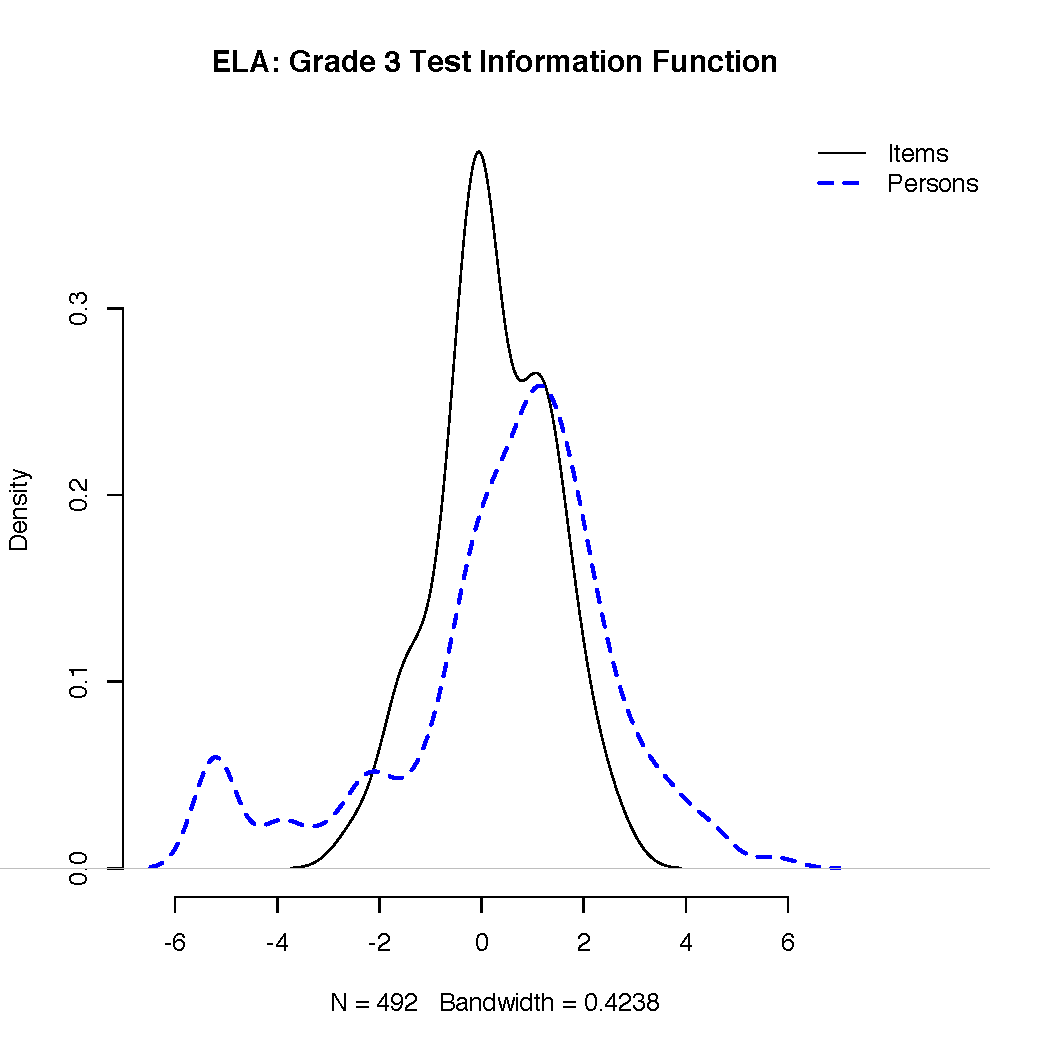
\includegraphics[width=\textwidth,height=3.125in]{ipdens/ela3ipdens.pdf}
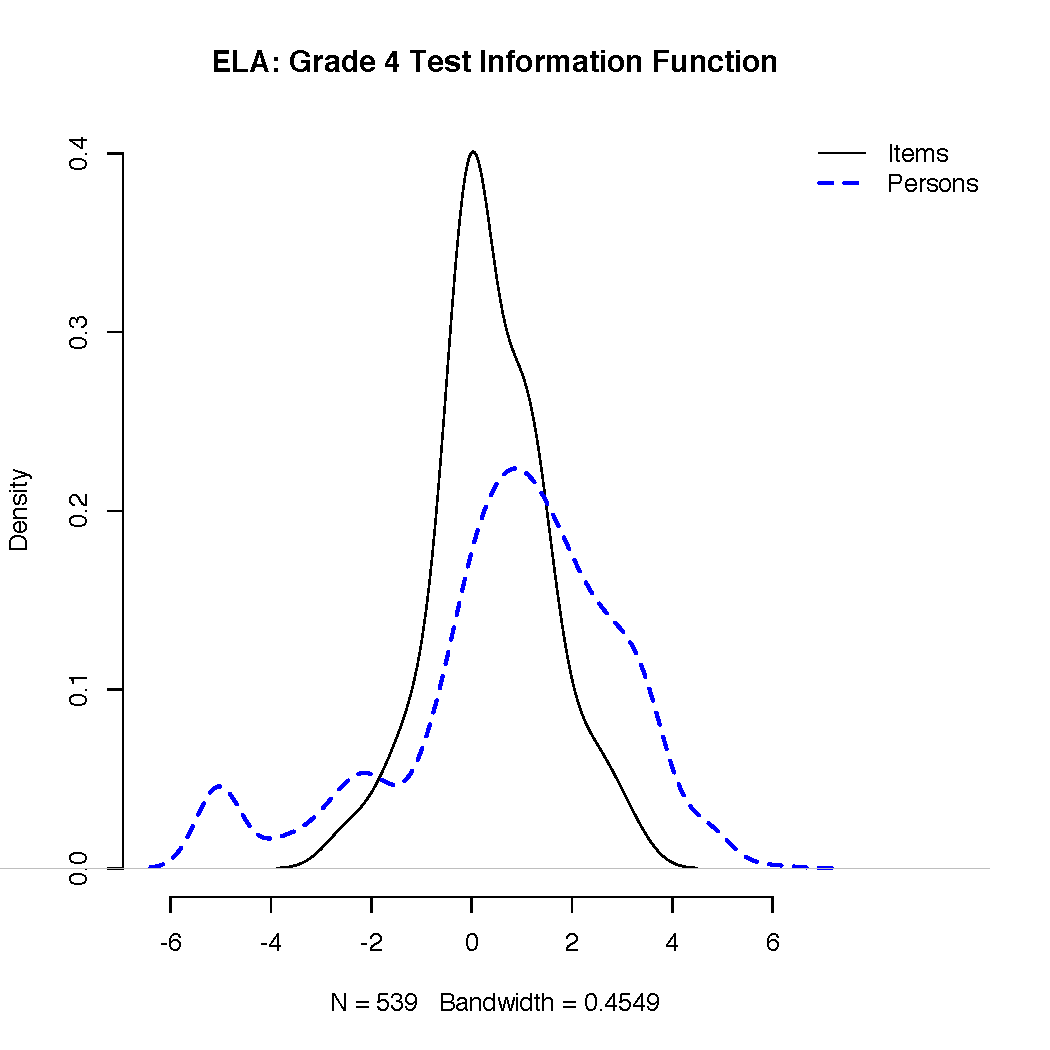
\includegraphics[width=\textwidth,height=3.125in]{ipdens/ela4ipdens.pdf}
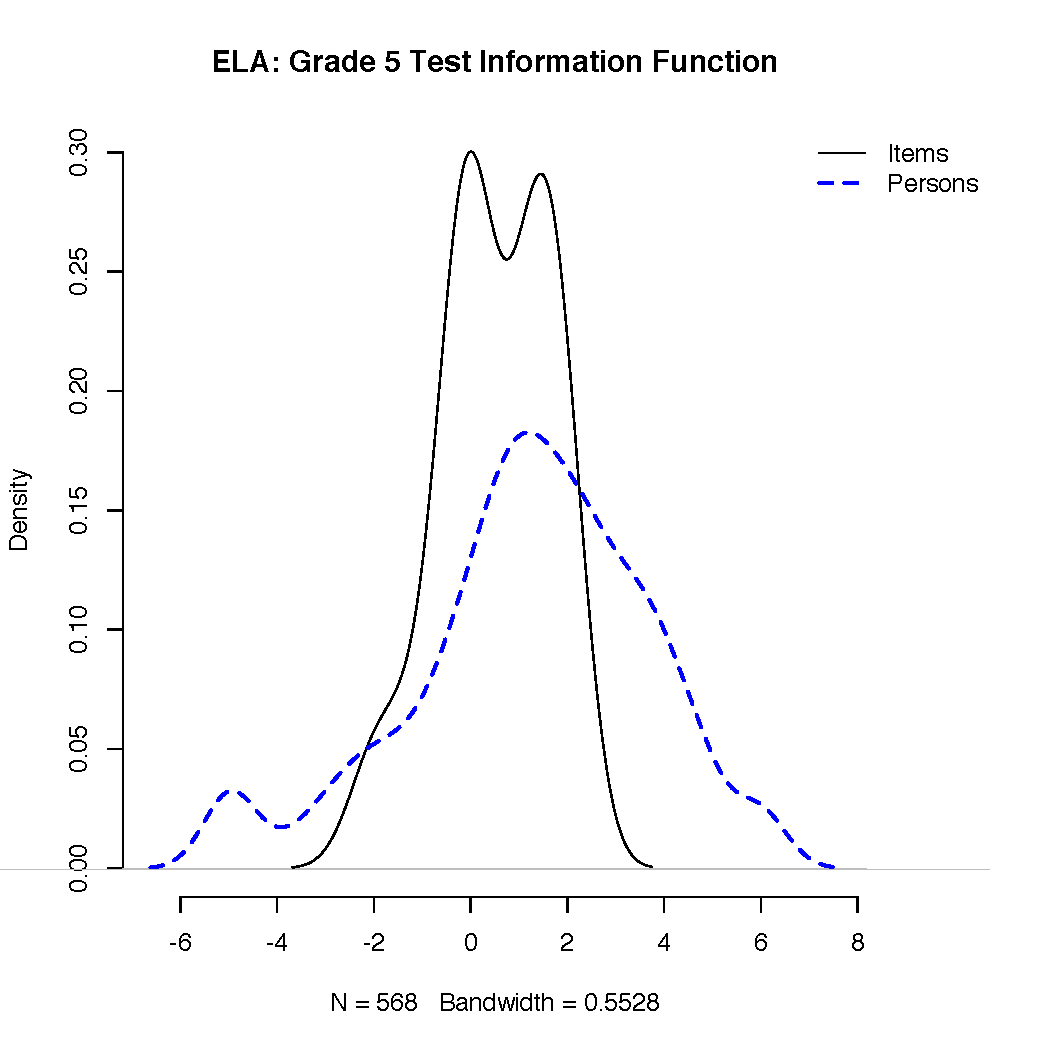
\includegraphics[width=\textwidth,height=3.125in]{ipdens/ela5ipdens.pdf}
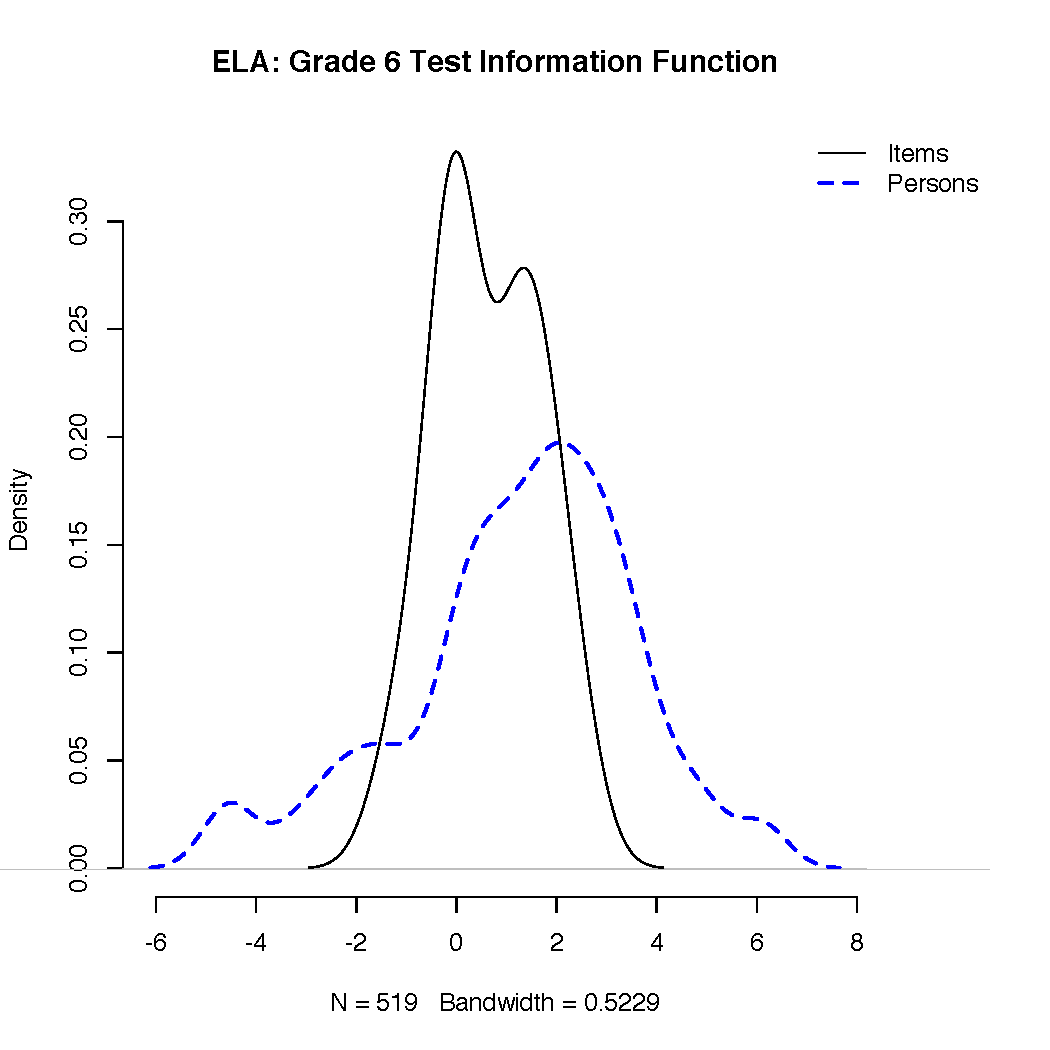
\includegraphics[width=\textwidth,height=3.125in]{ipdens/ela6ipdens.pdf}
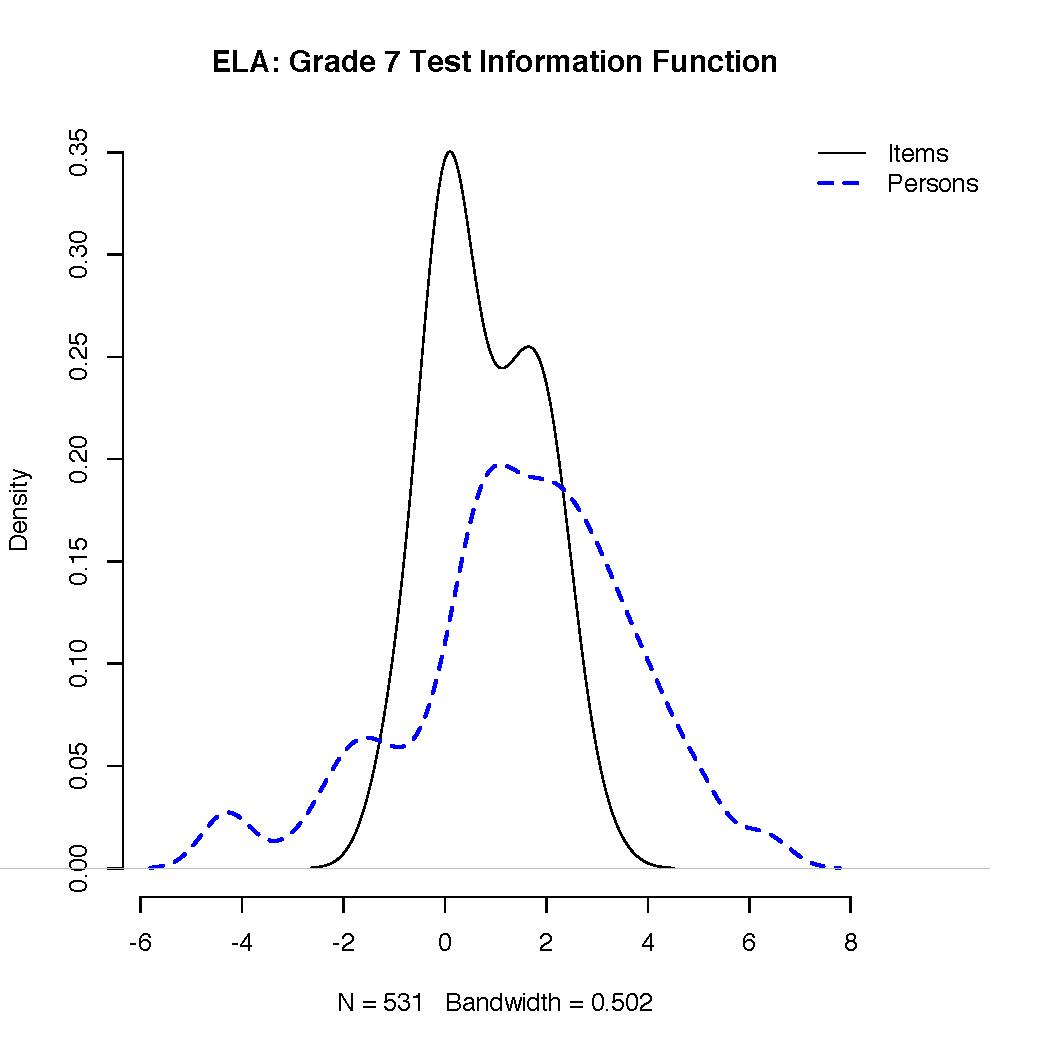
\includegraphics[width=\textwidth,height=3.125in]{ipdens/ela7ipdens.pdf}
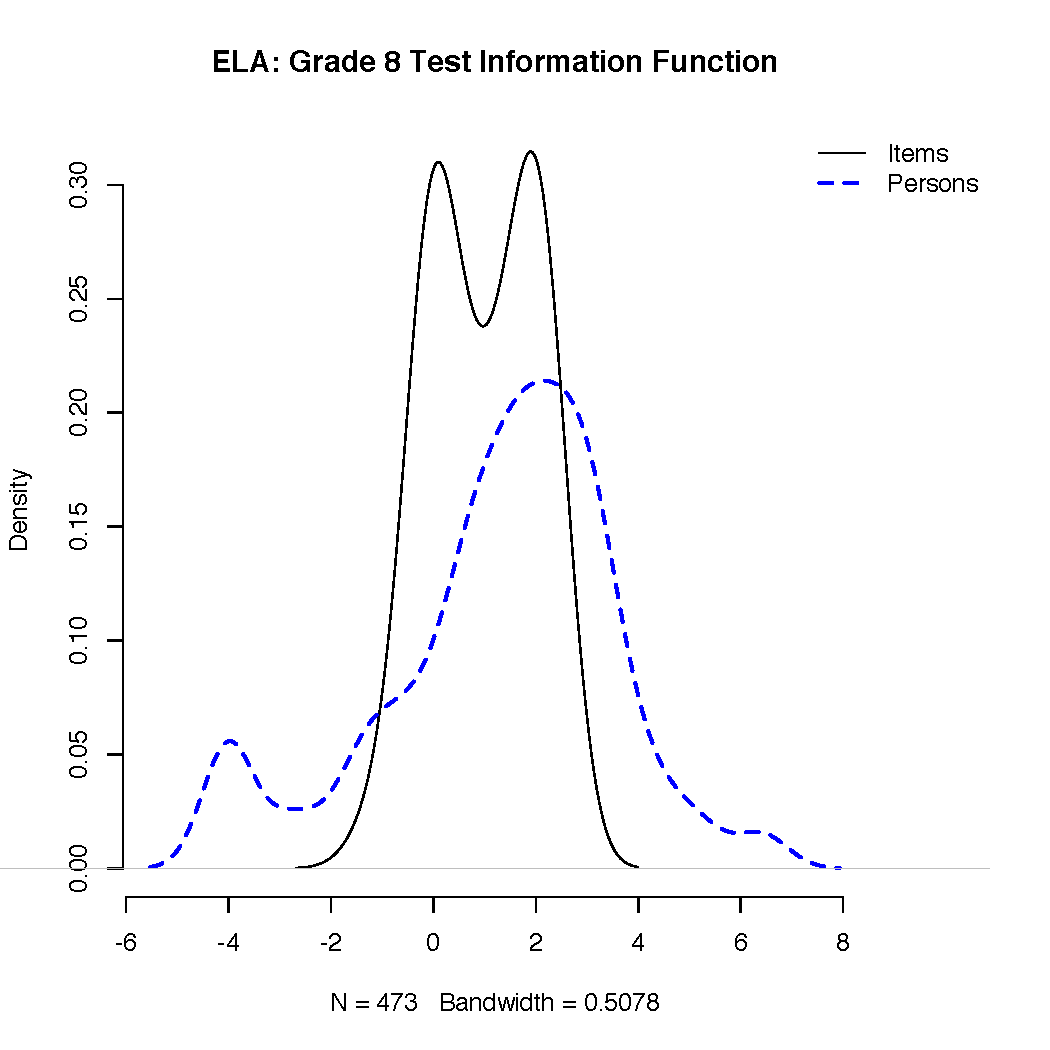
\includegraphics[width=\textwidth,height=3.125in]{ipdens/ela8ipdens.pdf}
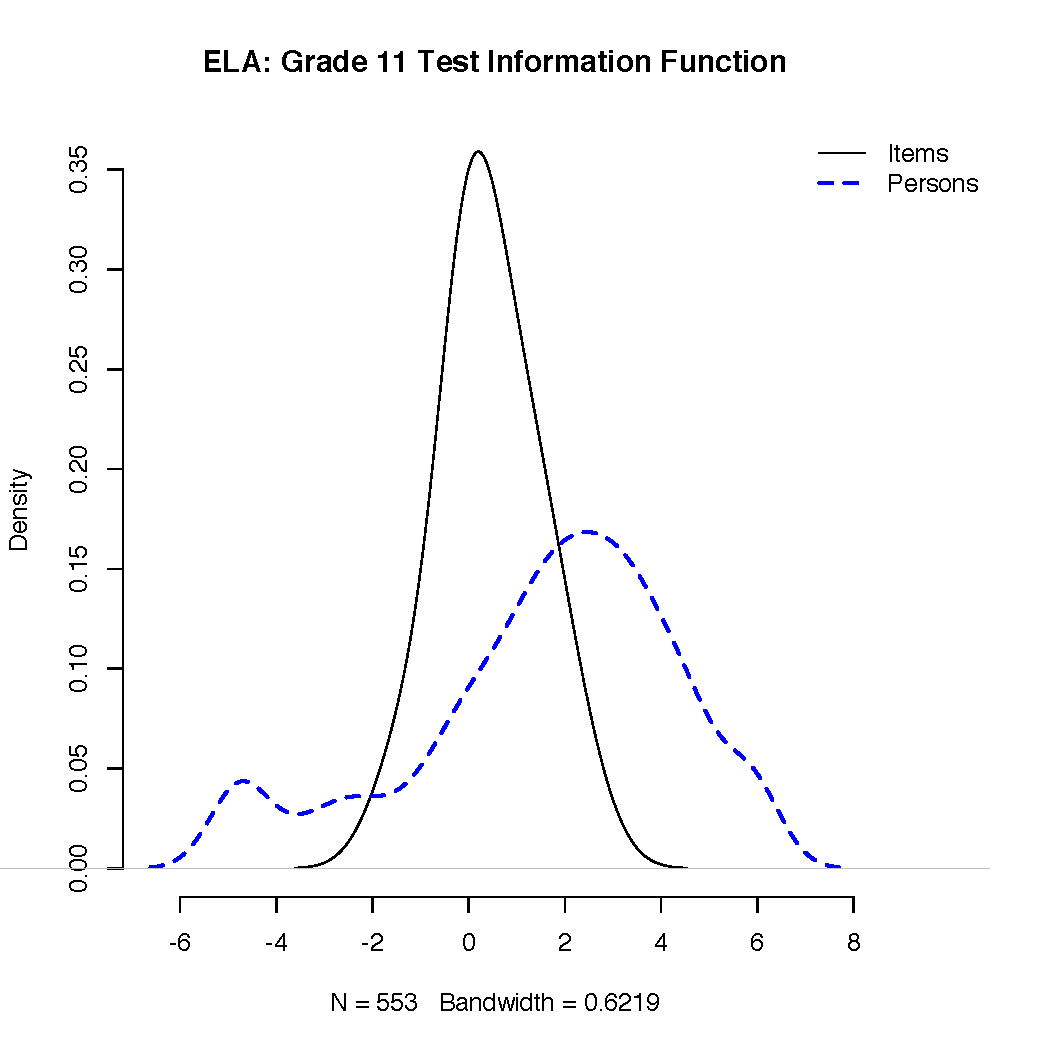
\includegraphics[width=\textwidth,height=3.125in]{ipdens/ela11ipdens.pdf}
\clearpage

\hypertarget{mathematics-personitem-distributions}{%
\paragraph{Mathematics Person/Item
Distributions}\label{mathematics-personitem-distributions}}

\FloatBarrier

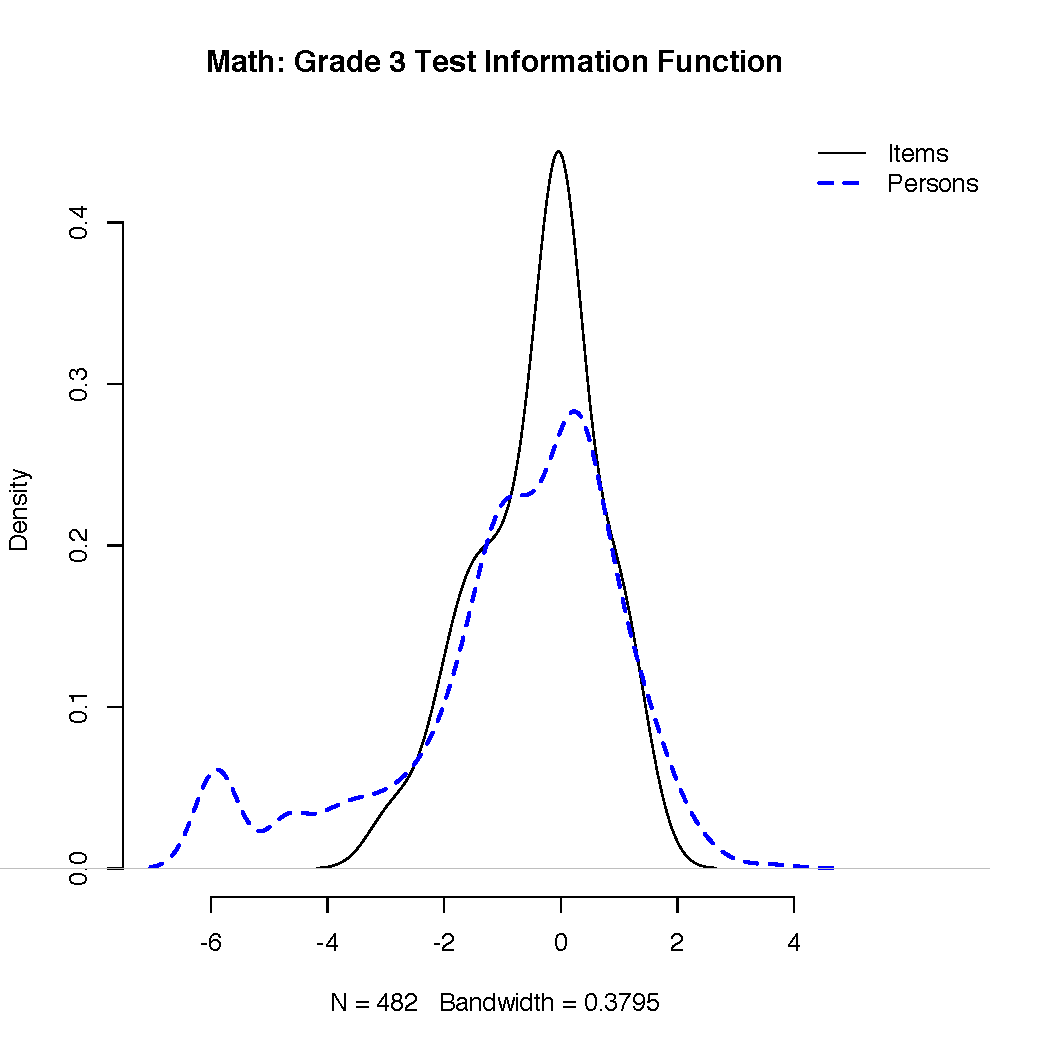
\includegraphics[width=\textwidth,height=3.125in]{ipdens/math3ipdens.pdf}
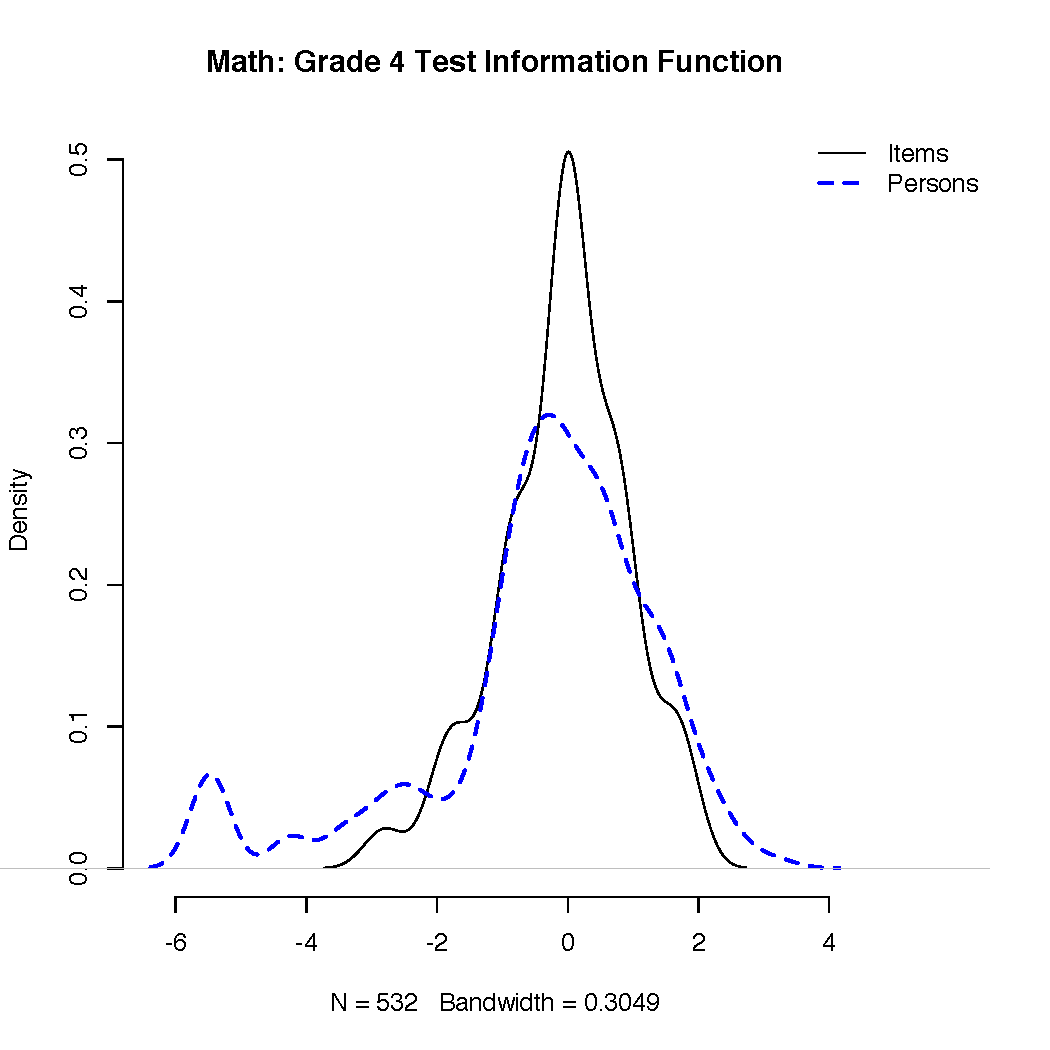
\includegraphics[width=\textwidth,height=3.125in]{ipdens/math4ipdens.pdf}
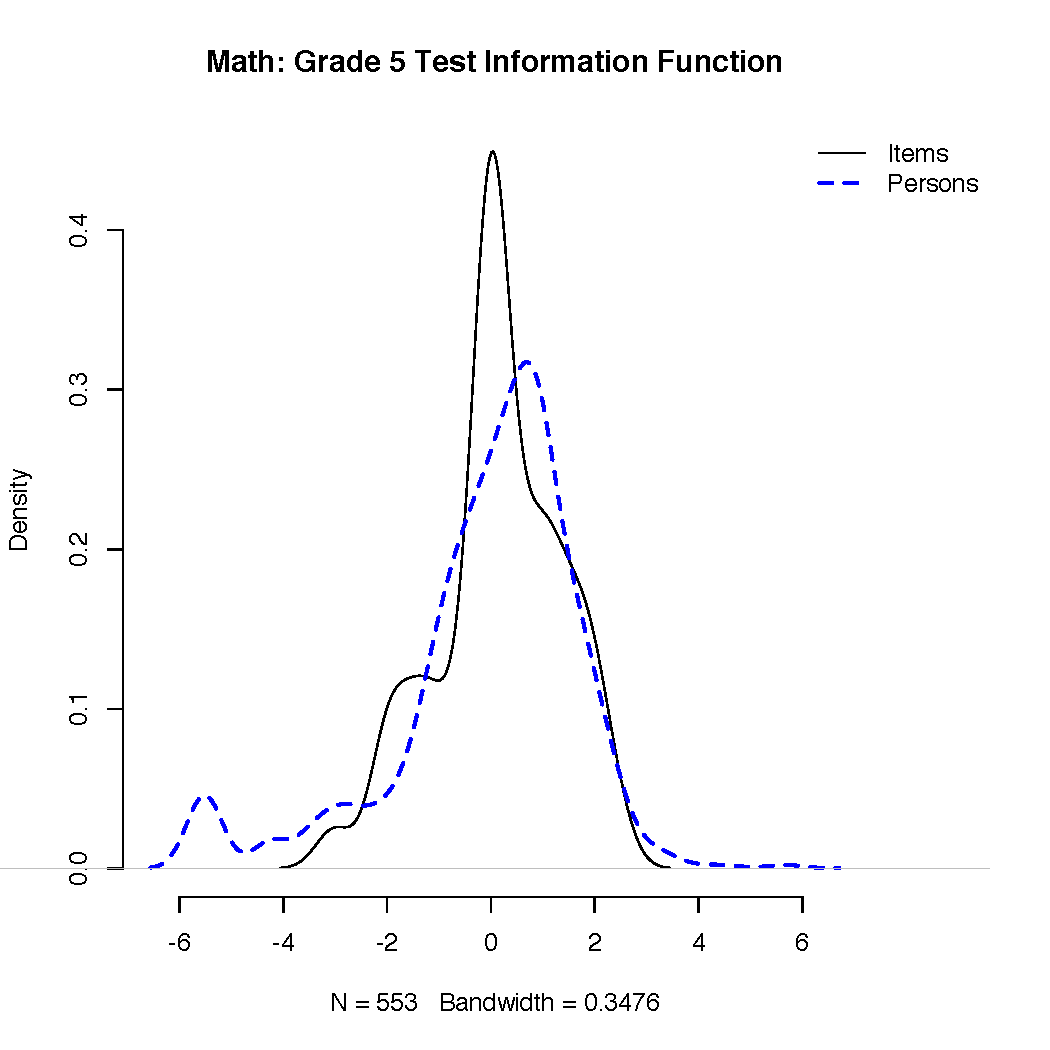
\includegraphics[width=\textwidth,height=3.125in]{ipdens/math5ipdens.pdf}
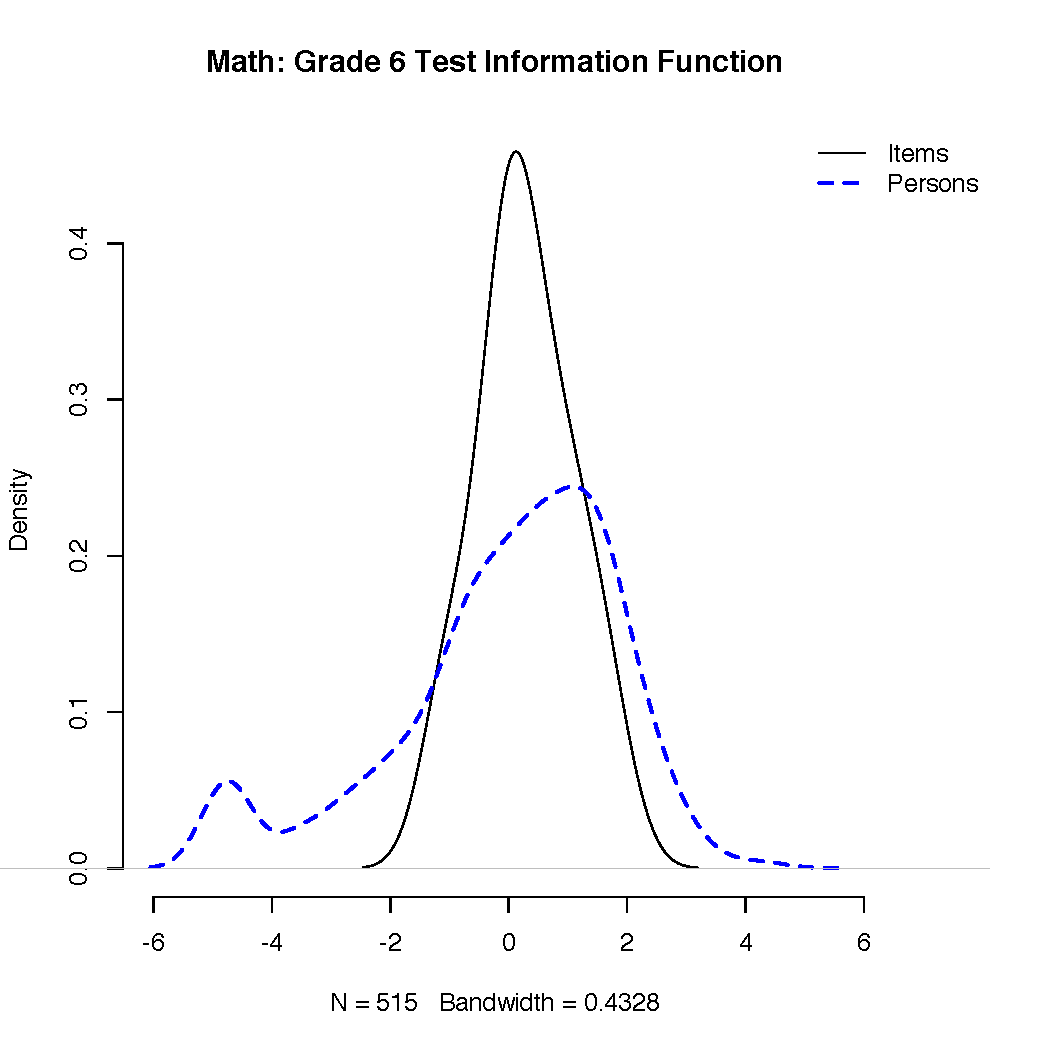
\includegraphics[width=\textwidth,height=3.125in]{ipdens/math6ipdens.pdf}
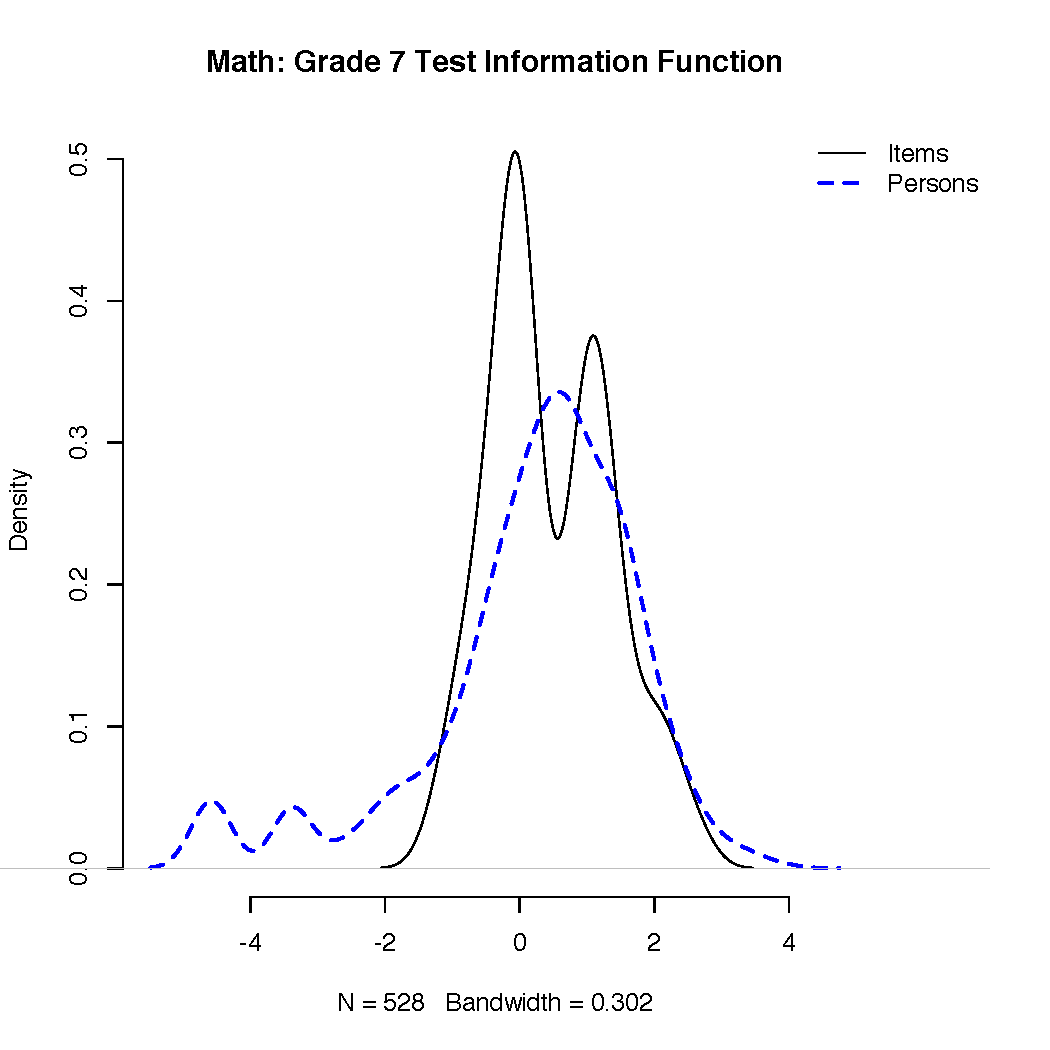
\includegraphics[width=\textwidth,height=3.125in]{ipdens/math7ipdens.pdf}
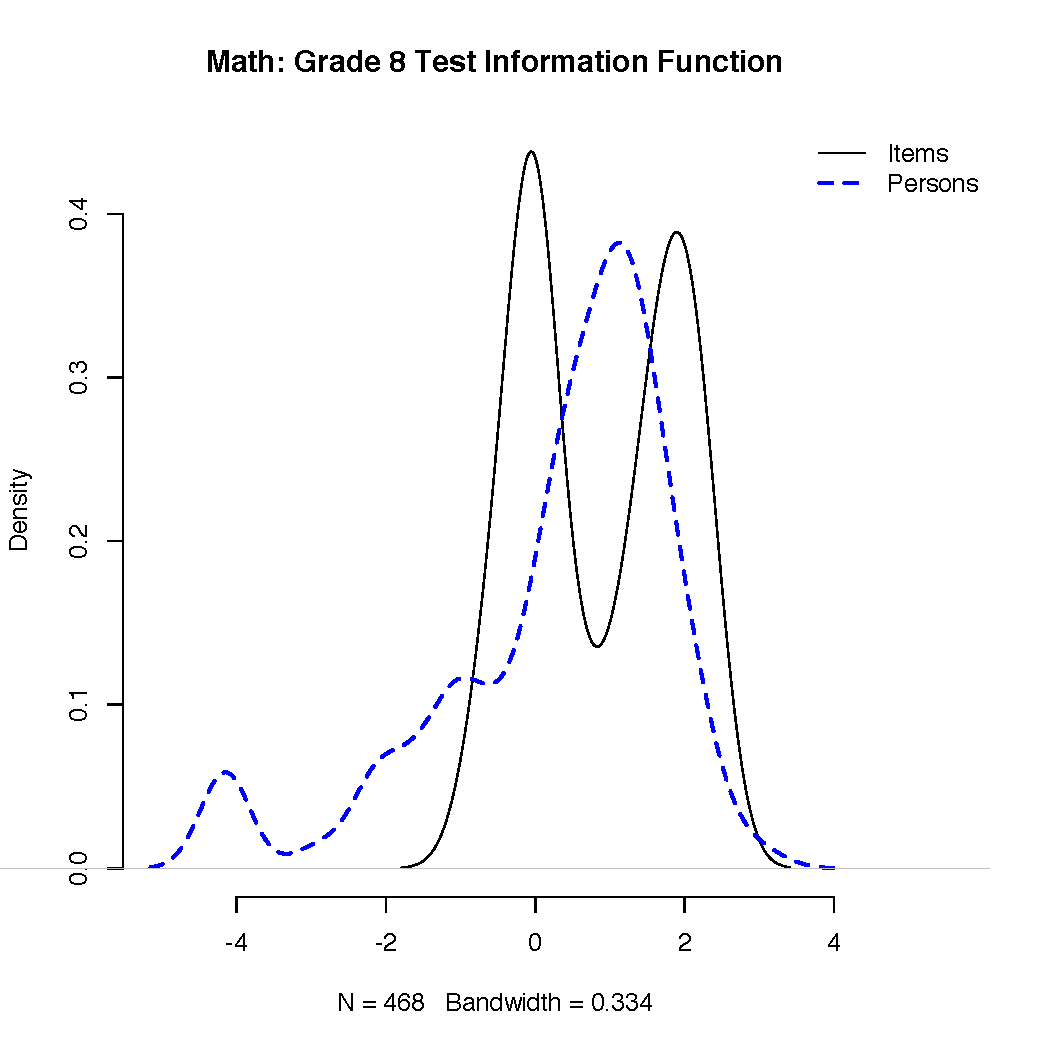
\includegraphics[width=\textwidth,height=3.125in]{ipdens/math8ipdens.pdf}
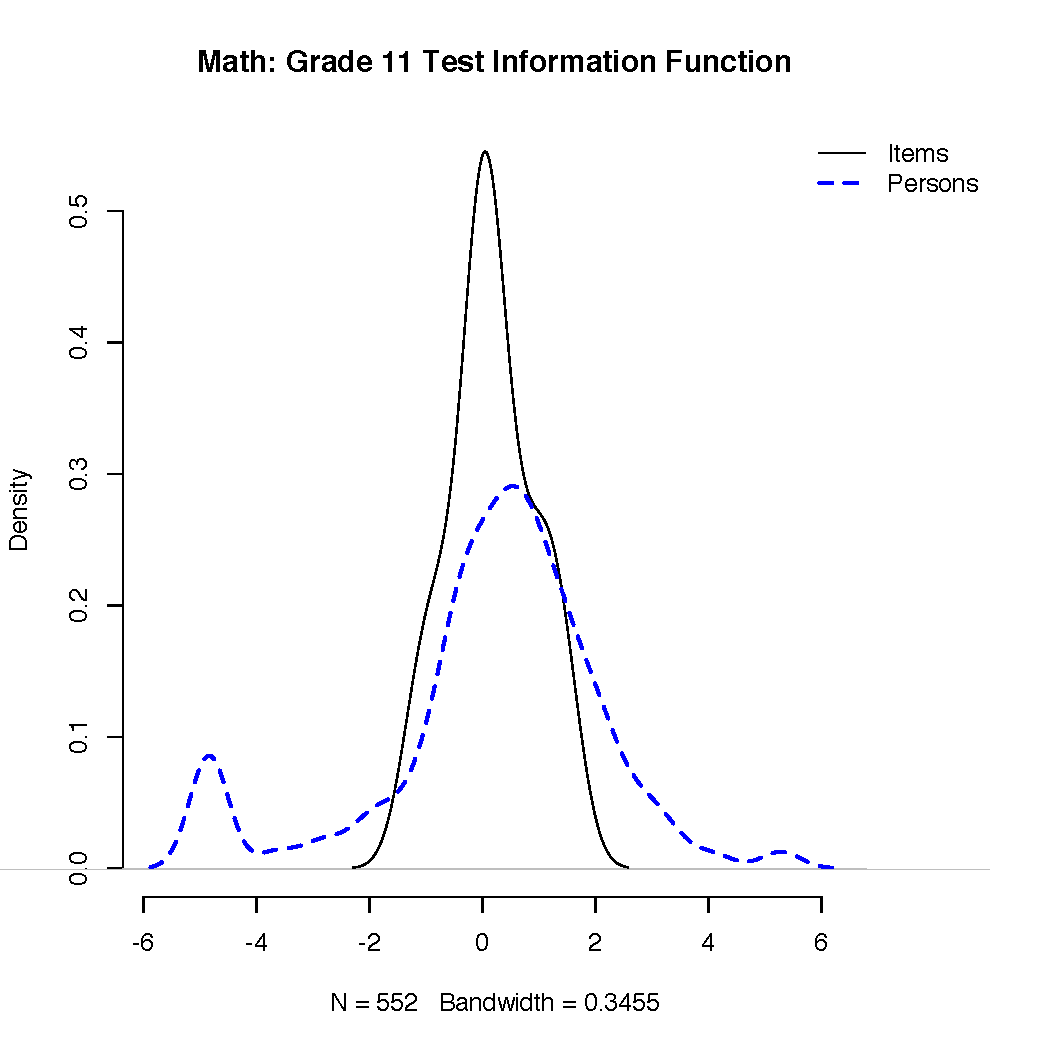
\includegraphics[width=\textwidth,height=3.125in]{ipdens/math11ipdens.pdf}
\clearpage

\hypertarget{science-personitem-distributions}{%
\paragraph{Science Person/Item
Distributions}\label{science-personitem-distributions}}

\FloatBarrier

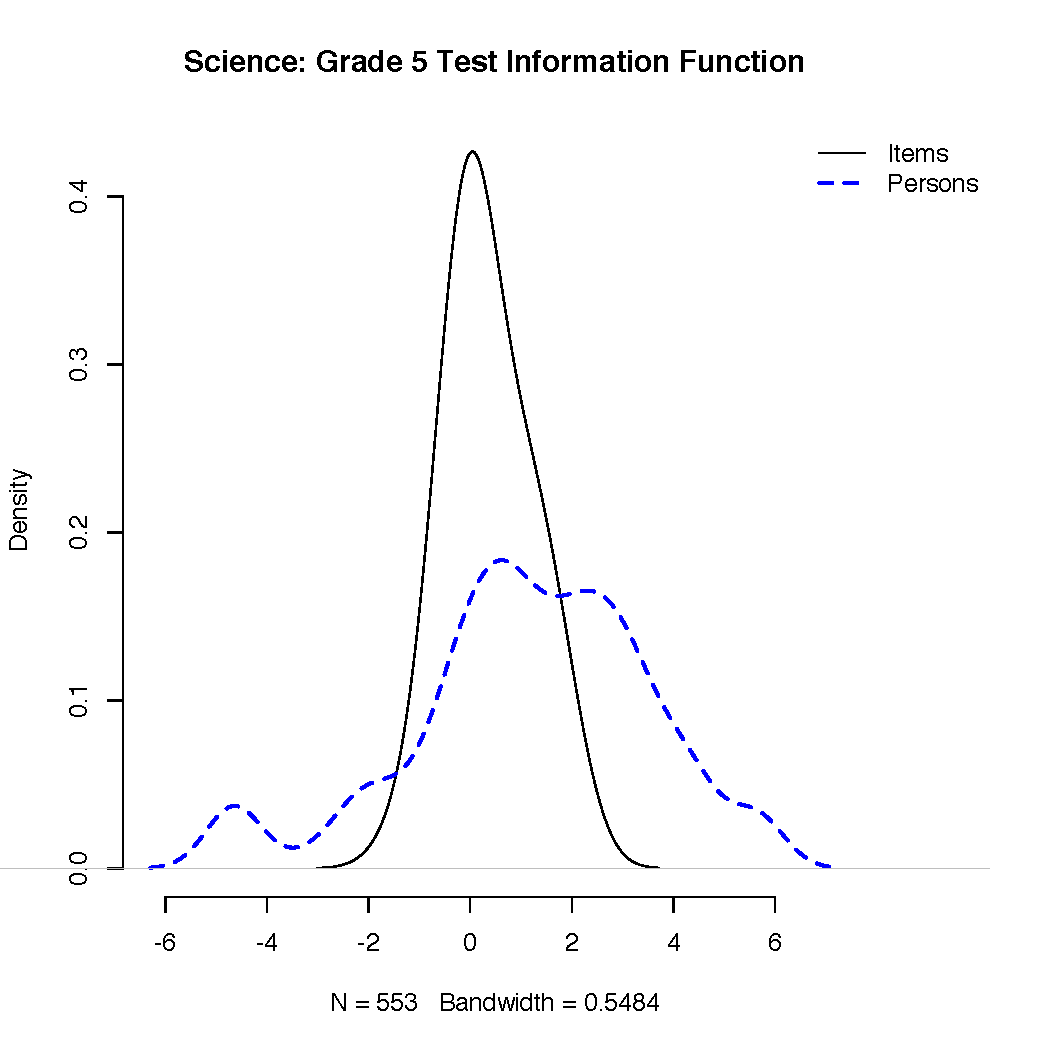
\includegraphics[width=\textwidth,height=3.125in]{ipdens/science5ipdens.pdf}
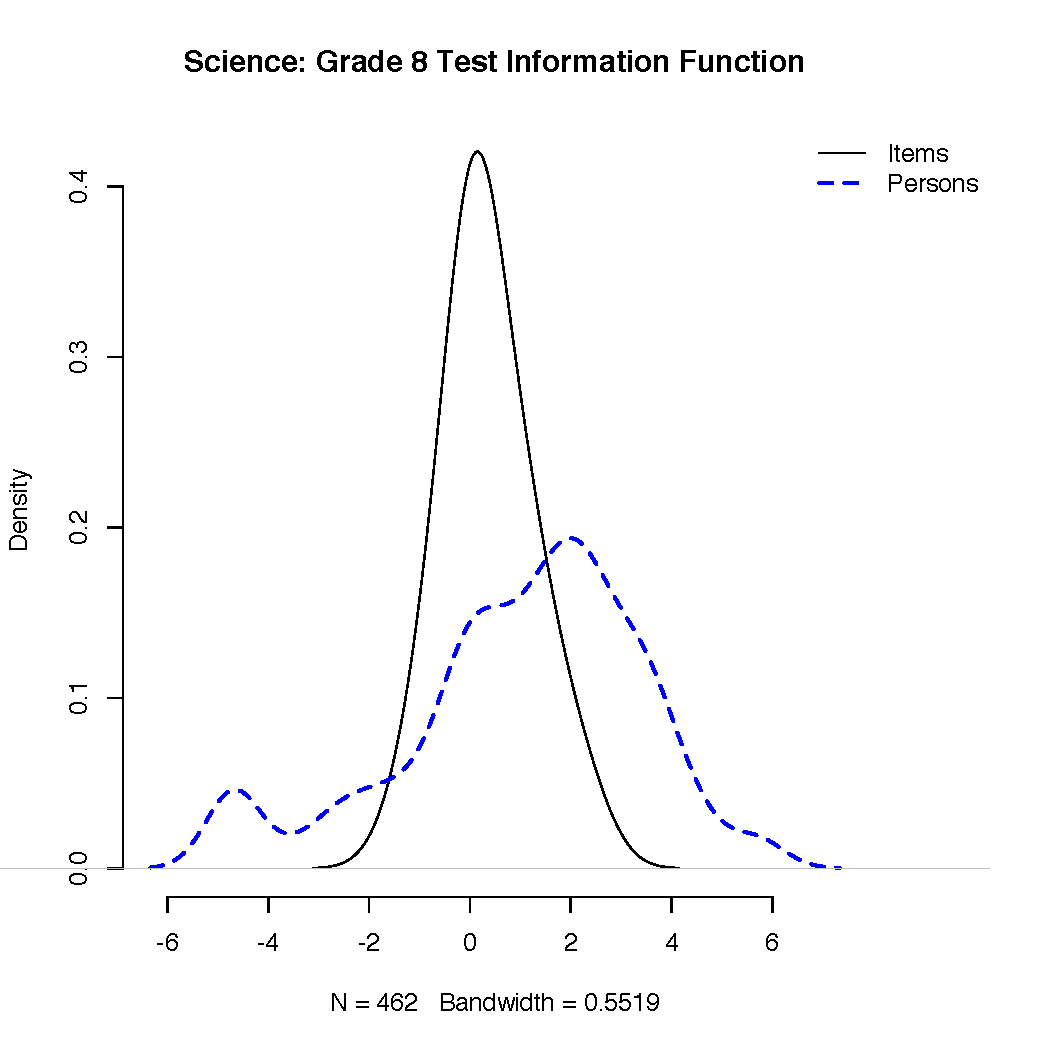
\includegraphics[width=\textwidth,height=3.125in]{ipdens/science8ipdens.pdf}
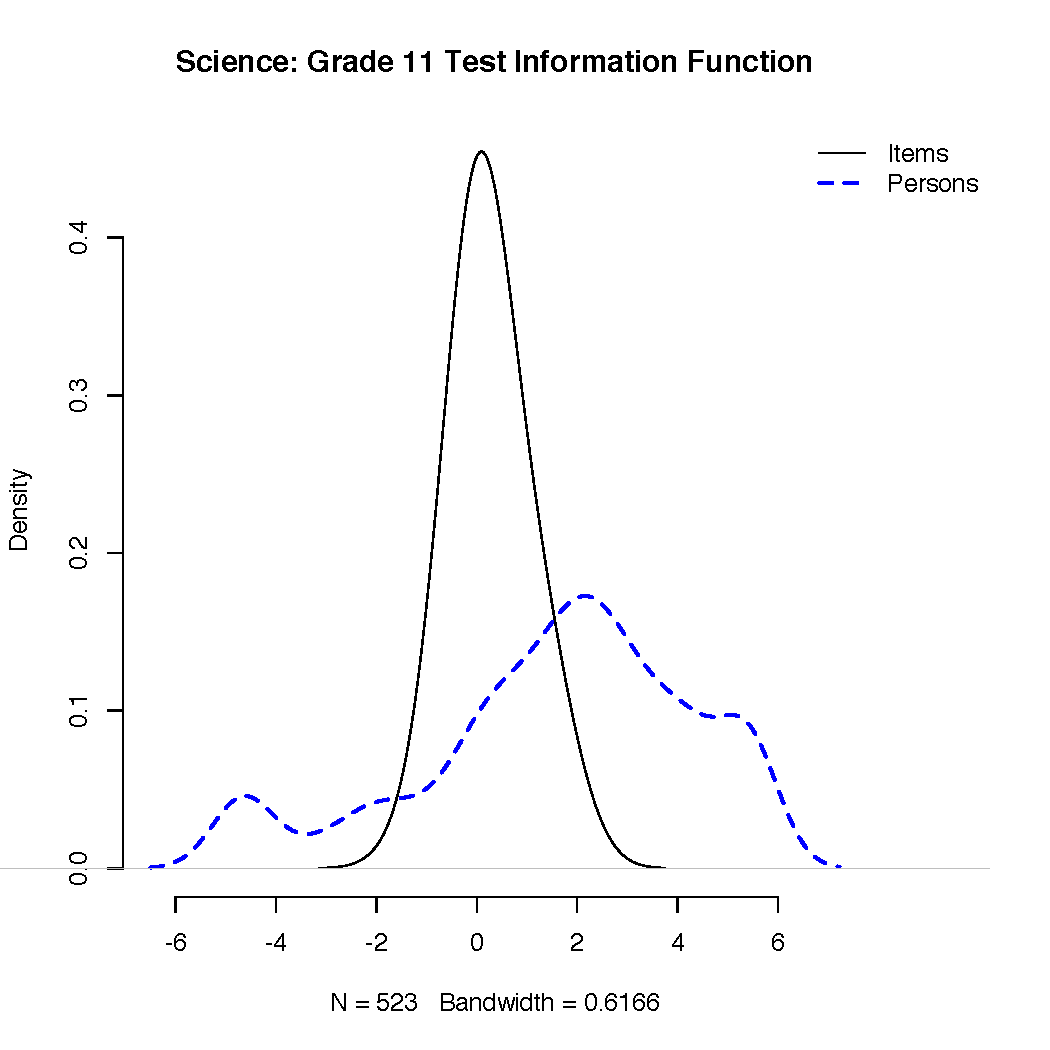
\includegraphics[width=\textwidth,height=3.125in]{ipdens/science11ipdens.pdf}

\hypertarget{scoring}{%
\subsubsection{4.4 Scoring}\label{scoring}}

All scoring expectations for the ORExt are established within the
Administration Manual (see \emph{Appendix} 2.3, p.~14). The scoring
procedures for the new ORExt have been simplified, with students
receiving a 0 for an incorrect response or a 1 for a correct response.
Input from the field gathered from Consequential Validity studies
demonstrates that the assessment scoring procedures are much more clear
and easier to implement than prior scoring approaches (see
\emph{Appendix} 2.3B.10). BRT was also commissioned to develop a scaled
score interpretation guide, which describes specific strategies for
interpreting student test scores and sub-test scores in Reading and
Writing, and Achievement Level Descriptors (ALDs) published within the
Individual Student Reports (see \emph{Appendix} 6.4C) for annual
performance, growth, and as part of Essential Skills requirements for
very low performing students (see \emph{Appendix} 2.1A).

\hypertarget{multiple-assessment-forms}{%
\subsubsection{4.5 Multiple Assessment
Forms}\label{multiple-assessment-forms}}

The ORExt was administered in only form per subject area and grade level
for the 2017-18 school year, with 36 operational items arranged in order
of empirical difficulty and 12 embedded field test items.

\hypertarget{multiple-versions-of-an-assessment}{%
\subsubsection{4.6 Multiple Versions of An
Assessment}\label{multiple-versions-of-an-assessment}}

The ORExt is provided in the standard format, but is also available in
Large Print and Brailled formats. Test content is identical across all
three versions, with an occasional item being eliminated on the Braille
version due to inaccessibility. These items do not count for or against
the student in reporting. Substantive test comparability analyses are
not feasible, given the small n-sizes of the samples involved in the
alternative versions.

\hypertarget{technical-analyses-and-ongoing-maintenance}{%
\subsubsection{4.7 Technical Analyses and Ongoing
Maintenance}\label{technical-analyses-and-ongoing-maintenance}}

The ORExt technical analyses that document reliability and validity are
included in this technical report (see Sections 3 and 4, respectively).
ODE and BRT staff review these analyses annually. Necessary adjustments
to the assessment are determined prior to implementation of the
subsequent year's work plan, which elaborates the areas of improvement
as well as aspects of the testing program that will be maintained. This
decision-making is supported by input from the field gathered from the
Consequential Validity study (see \emph{Appendix} 2.3B.10).

Within our system of ongoing improvement is continuation of the
development of additional curricular and instructional resources. This
addresses an area of concern expressed by stakeholders. Training modules
and templates continue to be developed to connect assessment results
from the ORExt and ORora with curricular resources and instructional
strategies aligned to the standards.


\end{document}
